\documentclass{book}
\usepackage[a4paper,top=2.5cm,bottom=2.5cm,left=2.5cm,right=2.5cm]{geometry}
\usepackage{makeidx}
\usepackage{natbib}
\usepackage{graphicx}
\usepackage{multicol}
\usepackage{float}
\usepackage{listings}
\usepackage{color}
\usepackage{ifthen}
\usepackage[table]{xcolor}
\usepackage{textcomp}
\usepackage{alltt}
\usepackage{ifpdf}
\ifpdf
\usepackage[pdftex,
            pagebackref=true,
            colorlinks=true,
            linkcolor=blue,
            unicode
           ]{hyperref}
\else
\usepackage[ps2pdf,
            pagebackref=true,
            colorlinks=true,
            linkcolor=blue,
            unicode
           ]{hyperref}
\usepackage{pspicture}
\fi
\usepackage[utf8]{inputenc}
\usepackage[french]{babel}

\usepackage{mathptmx}
\usepackage[scaled=.90]{helvet}
\usepackage{courier}
\usepackage{sectsty}
\usepackage{amssymb}
\usepackage[titles]{tocloft}
\usepackage{doxygen}
\lstset{language=C++,inputencoding=utf8,basicstyle=\footnotesize,breaklines=true,breakatwhitespace=true,tabsize=8,numbers=left }
\makeindex
\setcounter{tocdepth}{3}
\renewcommand{\footrulewidth}{0.4pt}
\renewcommand{\familydefault}{\sfdefault}
\hfuzz=15pt
\setlength{\emergencystretch}{15pt}
\hbadness=750
\tolerance=750
\begin{document}
\hypersetup{pageanchor=false,citecolor=blue}
\begin{titlepage}
\vspace*{7cm}
\begin{center}
{\Large Carré chinois \\[1ex]\large v1.\-0 }\\
\vspace*{1cm}
{\large Généré par Doxygen 1.8.1.2}\\
\vspace*{0.5cm}
{\small Lundi Décembre 9 2013 17:48:32}\\
\end{center}
\end{titlepage}
\clearemptydoublepage
\pagenumbering{roman}
\tableofcontents
\clearemptydoublepage
\pagenumbering{arabic}
\hypersetup{pageanchor=true,citecolor=blue}
\chapter{Liste des choses à faire}
\label{todo}
\hypertarget{todo}{}

\begin{DoxyRefList}
\item[\label{todo__todo000001}%
\hypertarget{todo__todo000001}{}%
Espace de nommage \hyperlink{namespace_ui}{Ui} ]coder l'envoi du message (socket...) 

gérer le bouton envoyer(griser ou non en fonction si le jeu est en réseau ou non) 
\end{DoxyRefList}
\chapter{Liste des bogues}
\label{bug}
\hypertarget{bug}{}

\begin{DoxyRefList}
\item[\label{bug__bug000001}%
\hypertarget{bug__bug000001}{}%
Espace de nommage \hyperlink{namespace_ui}{Ui} ]ferme l'application à l'appui du bouton envoyer 
\end{DoxyRefList}
\chapter{Index des espaces de nommage}
\section{Liste des espaces de nommage}
Liste de tous les espaces de nommage avec une brève description\-:\begin{DoxyCompactList}
\item\contentsline{section}{\hyperlink{namespaceorg}{org} }{\pageref{namespaceorg}}{}
\item\contentsline{section}{\hyperlink{namespaceorg_1_1qtproject}{org.\-qtproject} }{\pageref{namespaceorg_1_1qtproject}}{}
\item\contentsline{section}{\hyperlink{namespaceorg_1_1qtproject_1_1qt5}{org.\-qtproject.\-qt5} }{\pageref{namespaceorg_1_1qtproject_1_1qt5}}{}
\item\contentsline{section}{\hyperlink{namespaceorg_1_1qtproject_1_1qt5_1_1android}{org.\-qtproject.\-qt5.\-android} }{\pageref{namespaceorg_1_1qtproject_1_1qt5_1_1android}}{}
\item\contentsline{section}{\hyperlink{namespaceorg_1_1qtproject_1_1qt5_1_1android_1_1bindings}{org.\-qtproject.\-qt5.\-android.\-bindings} }{\pageref{namespaceorg_1_1qtproject_1_1qt5_1_1android_1_1bindings}}{}
\item\contentsline{section}{\hyperlink{namespace_ui}{Ui} \\*Classe help \char`\"{}help.\-h\char`\"{} }{\pageref{namespace_ui}}{}
\end{DoxyCompactList}

\chapter{Index des classes}
\section{Liste des classes}
Liste des classes, structures, unions et interfaces avec une brève description \-:\begin{DoxyCompactList}
\item\contentsline{section}{\hyperlink{classemplacement}{emplacement} \\*The emplacement class }{\pageref{classemplacement}}{}
\item\contentsline{section}{\hyperlink{classhelp}{help} \\*The help class }{\pageref{classhelp}}{}
\item\contentsline{section}{\hyperlink{classjoueur}{joueur} \\*Classe joueur \char`\"{}joueur.\-h\char`\"{} }{\pageref{classjoueur}}{}
\item\contentsline{section}{\hyperlink{class_main_window}{Main\-Window} \\*The \hyperlink{class_main_window}{Main\-Window} class }{\pageref{class_main_window}}{}
\item\contentsline{section}{\hyperlink{classorg_1_1qtproject_1_1qt5_1_1android_1_1bindings_1_1_qt_activity}{org.\-qtproject.\-qt5.\-android.\-bindings.\-Qt\-Activity} }{\pageref{classorg_1_1qtproject_1_1qt5_1_1android_1_1bindings_1_1_qt_activity}}{}
\item\contentsline{section}{\hyperlink{classorg_1_1qtproject_1_1qt5_1_1android_1_1bindings_1_1_qt_application}{org.\-qtproject.\-qt5.\-android.\-bindings.\-Qt\-Application} }{\pageref{classorg_1_1qtproject_1_1qt5_1_1android_1_1bindings_1_1_qt_application}}{}
\end{DoxyCompactList}

\chapter{Index des fichiers}
\section{Liste des fichiers}
Liste de tous les fichiers avec une brève description \-:\begin{DoxyCompactList}
\item\contentsline{section}{\hyperlink{emplacement_8cpp}{emplacement.\-cpp} }{\pageref{emplacement_8cpp}}{}
\item\contentsline{section}{\hyperlink{emplacement_8h}{emplacement.\-h} }{\pageref{emplacement_8h}}{}
\item\contentsline{section}{\hyperlink{help_8cpp}{help.\-cpp} }{\pageref{help_8cpp}}{}
\item\contentsline{section}{\hyperlink{help_8h}{help.\-h} }{\pageref{help_8h}}{}
\item\contentsline{section}{\hyperlink{joueur_8cpp}{joueur.\-cpp} }{\pageref{joueur_8cpp}}{}
\item\contentsline{section}{\hyperlink{joueur_8h}{joueur.\-h} }{\pageref{joueur_8h}}{}
\item\contentsline{section}{\hyperlink{main_8cpp}{main.\-cpp} }{\pageref{main_8cpp}}{}
\item\contentsline{section}{\hyperlink{mainwindow_8cpp}{mainwindow.\-cpp} }{\pageref{mainwindow_8cpp}}{}
\item\contentsline{section}{\hyperlink{mainwindow_8h}{mainwindow.\-h} }{\pageref{mainwindow_8h}}{}
\item\contentsline{section}{android/src/org/qtproject/qt5/android/bindings/\hyperlink{_qt_activity_8java}{Qt\-Activity.\-java} }{\pageref{_qt_activity_8java}}{}
\item\contentsline{section}{android/src/org/qtproject/qt5/android/bindings/\hyperlink{_qt_application_8java}{Qt\-Application.\-java} }{\pageref{_qt_application_8java}}{}
\end{DoxyCompactList}

\chapter{Documentation des espaces de nommage}
\hypertarget{namespaceorg}{\section{Paquetage org}
\label{namespaceorg}\index{org@{org}}
}
\subsection*{Espaces de nommage}
\begin{DoxyCompactItemize}
\item 
package \hyperlink{namespaceorg_1_1qtproject}{qtproject}
\end{DoxyCompactItemize}

\hypertarget{namespaceorg_1_1qtproject}{\section{Paquetage org.\-qtproject}
\label{namespaceorg_1_1qtproject}\index{org.\-qtproject@{org.\-qtproject}}
}
\subsection*{Espaces de nommage}
\begin{DoxyCompactItemize}
\item 
package \hyperlink{namespaceorg_1_1qtproject_1_1qt5}{qt5}
\end{DoxyCompactItemize}

\hypertarget{namespaceorg_1_1qtproject_1_1qt5}{\section{Paquetage org.\-qtproject.\-qt5}
\label{namespaceorg_1_1qtproject_1_1qt5}\index{org.\-qtproject.\-qt5@{org.\-qtproject.\-qt5}}
}
\subsection*{Espaces de nommage}
\begin{DoxyCompactItemize}
\item 
package \hyperlink{namespaceorg_1_1qtproject_1_1qt5_1_1android}{android}
\end{DoxyCompactItemize}

\hypertarget{namespaceorg_1_1qtproject_1_1qt5_1_1android}{\section{Paquetage org.\-qtproject.\-qt5.\-android}
\label{namespaceorg_1_1qtproject_1_1qt5_1_1android}\index{org.\-qtproject.\-qt5.\-android@{org.\-qtproject.\-qt5.\-android}}
}
\subsection*{Espaces de nommage}
\begin{DoxyCompactItemize}
\item 
package \hyperlink{namespaceorg_1_1qtproject_1_1qt5_1_1android_1_1bindings}{bindings}
\end{DoxyCompactItemize}

\hypertarget{namespaceorg_1_1qtproject_1_1qt5_1_1android_1_1bindings}{\section{Paquetage org.\-qtproject.\-qt5.\-android.\-bindings}
\label{namespaceorg_1_1qtproject_1_1qt5_1_1android_1_1bindings}\index{org.\-qtproject.\-qt5.\-android.\-bindings@{org.\-qtproject.\-qt5.\-android.\-bindings}}
}
\subsection*{Classes}
\begin{DoxyCompactItemize}
\item 
class \hyperlink{classorg_1_1qtproject_1_1qt5_1_1android_1_1bindings_1_1_qt_activity}{Qt\-Activity}
\item 
class \hyperlink{classorg_1_1qtproject_1_1qt5_1_1android_1_1bindings_1_1_qt_application}{Qt\-Application}
\end{DoxyCompactItemize}

\hypertarget{namespace_ui}{\section{Référence de l'espace de nommage Ui}
\label{namespace_ui}\index{Ui@{Ui}}
}


Classe help \char`\"{}help.\-h\char`\"{}.  




\subsection{Description détaillée}
Classe help \char`\"{}help.\-h\char`\"{}. Classe \hyperlink{class_main_window}{Main\-Window} \char`\"{}mainwindow.\-h\char`\"{}.

Cette classe est la classe help elle permet d'afficher les règles du jeu \begin{DoxyAuthor}{Auteur}
Nicolas Capiaumont 
\end{DoxyAuthor}
\begin{DoxyVersion}{Version}
1 
\end{DoxyVersion}
\begin{DoxyDate}{Date}
06/12/13 
\end{DoxyDate}
\begin{DoxyCopyright}{Copyright}
G\-N\-U Public License.
\end{DoxyCopyright}
Cette classe est la classe mainwindow de notre application jeu en réseau \begin{DoxyAuthor}{Auteur}
Nicolas Capiaumont 
\end{DoxyAuthor}
\begin{DoxyVersion}{Version}
1.\-0 
\end{DoxyVersion}
\begin{DoxyDate}{Date}
06/12/13 
\end{DoxyDate}
\begin{DoxyCopyright}{Copyright}
G\-N\-U Public License. 
\end{DoxyCopyright}
\begin{DoxyRefDesc}{A faire}
\item[\hyperlink{todo__todo000001}{A faire}]coder l'envoi du message (socket...) 

gérer le bouton envoyer(griser ou non en fonction si le jeu est en réseau ou non) \end{DoxyRefDesc}
\begin{DoxyRefDesc}{Bogue}
\item[\hyperlink{bug__bug000001}{Bogue}]ferme l'application à l'appui du bouton envoyer \end{DoxyRefDesc}

\chapter{Documentation des classes}
\hypertarget{classemplacement}{\section{Référence de la classe emplacement}
\label{classemplacement}\index{emplacement@{emplacement}}
}


The emplacement class.  




{\ttfamily \#include $<$emplacement.\-h$>$}



Graphe de collaboration de emplacement\-:\nopagebreak
\begin{figure}[H]
\begin{center}
\leavevmode
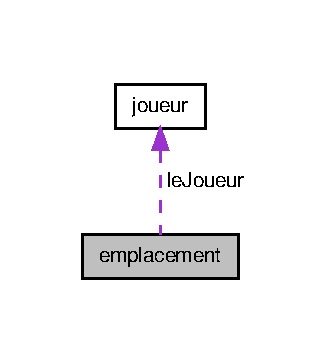
\includegraphics[width=157pt]{classemplacement__coll__graph}
\end{center}
\end{figure}
\subsection*{Connecteurs publics}
\begin{DoxyCompactItemize}
\item 
bool \hyperlink{classemplacement_afd15b612d02b7cbfd0480b5b380c2b07}{est\-Vide} ()
\begin{DoxyCompactList}\small\item\em bool \hyperlink{classemplacement_afd15b612d02b7cbfd0480b5b380c2b07}{est\-Vide()} \end{DoxyCompactList}\item 
bool \hyperlink{classemplacement_a70e22f75b934e4daa40582708c4e01f5}{jouxte} (\hyperlink{classemplacement}{emplacement} $\ast$e)
\begin{DoxyCompactList}\small\item\em bool \hyperlink{classemplacement_a70e22f75b934e4daa40582708c4e01f5}{jouxte(emplacement$\ast$ e)} \end{DoxyCompactList}\item 
void \hyperlink{classemplacement_a9e57590839f9c185d962030b221b8ea1}{set\-Joueur} (\hyperlink{classjoueur}{joueur} $\ast$)
\begin{DoxyCompactList}\small\item\em void \hyperlink{classemplacement_a9e57590839f9c185d962030b221b8ea1}{set\-Joueur(joueur$\ast$)} \end{DoxyCompactList}\item 
void \hyperlink{classemplacement_ada71fd6bec4969e4ef5be1a610d712a4}{vider} ()
\begin{DoxyCompactList}\small\item\em void \hyperlink{classemplacement_ada71fd6bec4969e4ef5be1a610d712a4}{vider()}  vide tous les emplacement sur le plateau (met les images des emplacements vide (rond noir)) \end{DoxyCompactList}\end{DoxyCompactItemize}
\subsection*{Fonctions membres publiques}
\begin{DoxyCompactItemize}
\item 
\hyperlink{classemplacement_af7af55d84628659a8f0ebb01a6af128e}{emplacement} (\hyperlink{class_main_window}{Main\-Window} $\ast$maman, Q\-String texte, Q\-Widget $\ast$parent=0)
\begin{DoxyCompactList}\small\item\em explicit emplacement(\hyperlink{class_main_window}{Main\-Window} $\ast$ maman,Q\-String texte,Q\-Widget $\ast$parent = 0) \end{DoxyCompactList}\end{DoxyCompactItemize}
\subsection*{Attributs publics}
\begin{DoxyCompactItemize}
\item 
int \hyperlink{classemplacement_aa0e8e131a1d8325f2245c56f8d2e6e8c}{ligne}
\begin{DoxyCompactList}\small\item\em ligne \end{DoxyCompactList}\item 
int \hyperlink{classemplacement_ac0af10e9e8d40e815a8b9633019406b1}{col}
\begin{DoxyCompactList}\small\item\em col \end{DoxyCompactList}\item 
\hyperlink{classjoueur}{joueur} $\ast$ \hyperlink{classemplacement_a8d9cb5aac12931bb041590456f3b4544}{le\-Joueur}
\begin{DoxyCompactList}\small\item\em le\-Joueur \end{DoxyCompactList}\end{DoxyCompactItemize}


\subsection{Description détaillée}
The emplacement class. 

Définition à la ligne 18 du fichier emplacement.\-h.



\subsection{Documentation des constructeurs et destructeur}
\hypertarget{classemplacement_af7af55d84628659a8f0ebb01a6af128e}{\index{emplacement@{emplacement}!emplacement@{emplacement}}
\index{emplacement@{emplacement}!emplacement@{emplacement}}
\subsubsection[{emplacement}]{\setlength{\rightskip}{0pt plus 5cm}emplacement\-::emplacement (
\begin{DoxyParamCaption}
\item[{{\bf Main\-Window} $\ast$}]{maman, }
\item[{Q\-String}]{texte, }
\item[{Q\-Widget $\ast$}]{parent = {\ttfamily 0}}
\end{DoxyParamCaption}
)\hspace{0.3cm}{\ttfamily [explicit]}}}\label{classemplacement_af7af55d84628659a8f0ebb01a6af128e}


explicit emplacement(\hyperlink{class_main_window}{Main\-Window} $\ast$ maman,Q\-String texte,Q\-Widget $\ast$parent = 0) 


\begin{DoxyParams}{Paramètres}
{\em \hyperlink{class_main_window}{Main\-Window}} & maman \\
\hline
{\em Q\-String} & texte \\
\hline
{\em Q\-Widget} & parent \\
\hline
\end{DoxyParams}


Définition à la ligne 6 du fichier emplacement.\-cpp.



\subsection{Documentation des fonctions membres}
\hypertarget{classemplacement_afd15b612d02b7cbfd0480b5b380c2b07}{\index{emplacement@{emplacement}!est\-Vide@{est\-Vide}}
\index{est\-Vide@{est\-Vide}!emplacement@{emplacement}}
\subsubsection[{est\-Vide}]{\setlength{\rightskip}{0pt plus 5cm}bool emplacement\-::est\-Vide (
\begin{DoxyParamCaption}
{}
\end{DoxyParamCaption}
)\hspace{0.3cm}{\ttfamily [slot]}}}\label{classemplacement_afd15b612d02b7cbfd0480b5b380c2b07}


bool \hyperlink{classemplacement_afd15b612d02b7cbfd0480b5b380c2b07}{est\-Vide()} 

\begin{DoxyReturn}{Renvoie}
renvoie vrai si l'emplacement est vide  indique sur l'emplacement est vide ou non 
\end{DoxyReturn}


Définition à la ligne 13 du fichier emplacement.\-cpp.

\hypertarget{classemplacement_a70e22f75b934e4daa40582708c4e01f5}{\index{emplacement@{emplacement}!jouxte@{jouxte}}
\index{jouxte@{jouxte}!emplacement@{emplacement}}
\subsubsection[{jouxte}]{\setlength{\rightskip}{0pt plus 5cm}bool emplacement\-::jouxte (
\begin{DoxyParamCaption}
\item[{{\bf emplacement} $\ast$}]{e}
\end{DoxyParamCaption}
)\hspace{0.3cm}{\ttfamily [slot]}}}\label{classemplacement_a70e22f75b934e4daa40582708c4e01f5}


bool \hyperlink{classemplacement_a70e22f75b934e4daa40582708c4e01f5}{jouxte(emplacement$\ast$ e)} 


\begin{DoxyParams}{Paramètres}
{\em emplacement} & e \\
\hline
\end{DoxyParams}
\begin{DoxyReturn}{Renvoie}
renvoie vrai si l'emplacement en cours est à côté de l'emplacement e  indique si l'emplacement est vide a coté du jeton selectionné 
\end{DoxyReturn}


Définition à la ligne 131 du fichier emplacement.\-cpp.

\hypertarget{classemplacement_a9e57590839f9c185d962030b221b8ea1}{\index{emplacement@{emplacement}!set\-Joueur@{set\-Joueur}}
\index{set\-Joueur@{set\-Joueur}!emplacement@{emplacement}}
\subsubsection[{set\-Joueur}]{\setlength{\rightskip}{0pt plus 5cm}void emplacement\-::set\-Joueur (
\begin{DoxyParamCaption}
\item[{{\bf joueur} $\ast$}]{j}
\end{DoxyParamCaption}
)\hspace{0.3cm}{\ttfamily [slot]}}}\label{classemplacement_a9e57590839f9c185d962030b221b8ea1}


void \hyperlink{classemplacement_a9e57590839f9c185d962030b221b8ea1}{set\-Joueur(joueur$\ast$)} 



Définition à la ligne 22 du fichier emplacement.\-cpp.

\hypertarget{classemplacement_ada71fd6bec4969e4ef5be1a610d712a4}{\index{emplacement@{emplacement}!vider@{vider}}
\index{vider@{vider}!emplacement@{emplacement}}
\subsubsection[{vider}]{\setlength{\rightskip}{0pt plus 5cm}void emplacement\-::vider (
\begin{DoxyParamCaption}
{}
\end{DoxyParamCaption}
)\hspace{0.3cm}{\ttfamily [slot]}}}\label{classemplacement_ada71fd6bec4969e4ef5be1a610d712a4}


void \hyperlink{classemplacement_ada71fd6bec4969e4ef5be1a610d712a4}{vider()}  vide tous les emplacement sur le plateau (met les images des emplacements vide (rond noir)) 



Définition à la ligne 17 du fichier emplacement.\-cpp.



\subsection{Documentation des données membres}
\hypertarget{classemplacement_ac0af10e9e8d40e815a8b9633019406b1}{\index{emplacement@{emplacement}!col@{col}}
\index{col@{col}!emplacement@{emplacement}}
\subsubsection[{col}]{\setlength{\rightskip}{0pt plus 5cm}int emplacement\-::col}}\label{classemplacement_ac0af10e9e8d40e815a8b9633019406b1}


col 



Définition à la ligne 50 du fichier emplacement.\-h.

\hypertarget{classemplacement_a8d9cb5aac12931bb041590456f3b4544}{\index{emplacement@{emplacement}!le\-Joueur@{le\-Joueur}}
\index{le\-Joueur@{le\-Joueur}!emplacement@{emplacement}}
\subsubsection[{le\-Joueur}]{\setlength{\rightskip}{0pt plus 5cm}{\bf joueur} $\ast$ emplacement\-::le\-Joueur}}\label{classemplacement_a8d9cb5aac12931bb041590456f3b4544}


le\-Joueur 



Définition à la ligne 55 du fichier emplacement.\-h.

\hypertarget{classemplacement_aa0e8e131a1d8325f2245c56f8d2e6e8c}{\index{emplacement@{emplacement}!ligne@{ligne}}
\index{ligne@{ligne}!emplacement@{emplacement}}
\subsubsection[{ligne}]{\setlength{\rightskip}{0pt plus 5cm}int emplacement\-::ligne}}\label{classemplacement_aa0e8e131a1d8325f2245c56f8d2e6e8c}


ligne 



Définition à la ligne 45 du fichier emplacement.\-h.



La documentation de cette classe a été générée à partir des fichiers suivants \-:\begin{DoxyCompactItemize}
\item 
\hyperlink{emplacement_8h}{emplacement.\-h}\item 
\hyperlink{emplacement_8cpp}{emplacement.\-cpp}\end{DoxyCompactItemize}

\hypertarget{classhelp}{\section{Référence de la classe help}
\label{classhelp}\index{help@{help}}
}


The help class.  




{\ttfamily \#include $<$help.\-h$>$}

\subsection*{Fonctions membres publiques}
\begin{DoxyCompactItemize}
\item 
\hyperlink{classhelp_a5bfcc97f9332fc089a54fd2bcfe43b1b}{help} (Q\-Widget $\ast$parent=0)
\item 
\hyperlink{classhelp_a390de3ebd37e8a7070992d9e642e70f5}{$\sim$help} ()
\begin{DoxyCompactList}\small\item\em Le destructeur. \end{DoxyCompactList}\end{DoxyCompactItemize}


\subsection{Description détaillée}
The help class. 

Définition à la ligne 19 du fichier help.\-h.



\subsection{Documentation des constructeurs et destructeur}
\hypertarget{classhelp_a5bfcc97f9332fc089a54fd2bcfe43b1b}{\index{help@{help}!help@{help}}
\index{help@{help}!help@{help}}
\subsubsection[{help}]{\setlength{\rightskip}{0pt plus 5cm}help\-::help (
\begin{DoxyParamCaption}
\item[{Q\-Widget $\ast$}]{parent = {\ttfamily 0}}
\end{DoxyParamCaption}
)\hspace{0.3cm}{\ttfamily [explicit]}}}\label{classhelp_a5bfcc97f9332fc089a54fd2bcfe43b1b}


Définition à la ligne 3 du fichier help.\-cpp.

\hypertarget{classhelp_a390de3ebd37e8a7070992d9e642e70f5}{\index{help@{help}!$\sim$help@{$\sim$help}}
\index{$\sim$help@{$\sim$help}!help@{help}}
\subsubsection[{$\sim$help}]{\setlength{\rightskip}{0pt plus 5cm}help\-::$\sim$help (
\begin{DoxyParamCaption}
{}
\end{DoxyParamCaption}
)}}\label{classhelp_a390de3ebd37e8a7070992d9e642e70f5}


Le destructeur. 

Le destructeur détruit l'instance et libère la mémoire allouée dynamiquement 

Définition à la ligne 9 du fichier help.\-cpp.



La documentation de cette classe a été générée à partir des fichiers suivants \-:\begin{DoxyCompactItemize}
\item 
\hyperlink{help_8h}{help.\-h}\item 
\hyperlink{help_8cpp}{help.\-cpp}\end{DoxyCompactItemize}

\hypertarget{classjoueur}{\section{Référence de la classe joueur}
\label{classjoueur}\index{joueur@{joueur}}
}


Classe joueur \char`\"{}joueur.\-h\char`\"{}.  




{\ttfamily \#include $<$joueur.\-h$>$}

\subsection*{Connecteurs publics}
\begin{DoxyCompactItemize}
\item 
void \hyperlink{classjoueur_a6c718c04f1db54452e366aeaddeb249d}{sur\-Brille} (bool active)
\begin{DoxyCompactList}\small\item\em void \hyperlink{classjoueur_a6c718c04f1db54452e366aeaddeb249d}{sur\-Brille(bool active)} \end{DoxyCompactList}\end{DoxyCompactItemize}
\subsection*{Fonctions membres publiques}
\begin{DoxyCompactItemize}
\item 
\hyperlink{classjoueur_a9f78a65e07011114967ef5c813a868cb}{joueur} (Q\-String l, Q\-String string\-Couleur, Q\-Widget $\ast$parent=0)
\begin{DoxyCompactList}\small\item\em explicit joueur(Q\-String l,Q\-String string\-Couleur, Q\-Widget $\ast$parent = 0) \end{DoxyCompactList}\item 
void \hyperlink{classjoueur_a6095d00e5c84a98694ae3f2ebbef48d8}{set\-Lettre} (Q\-String)
\begin{DoxyCompactList}\small\item\em void \hyperlink{classjoueur_a6095d00e5c84a98694ae3f2ebbef48d8}{set\-Lettre(\-Q\-String)}  change la lettre du joueur \end{DoxyCompactList}\item 
Q\-String \hyperlink{classjoueur_a7a91ed8fa89ad62545bae8e805565c39}{get\-Lettre} ()
\begin{DoxyCompactList}\small\item\em Q\-String \hyperlink{classjoueur_a7a91ed8fa89ad62545bae8e805565c39}{get\-Lettre()} \end{DoxyCompactList}\item 
Q\-Cursor $\ast$ \hyperlink{classjoueur_a19403939c10d9a70b6035024978ca230}{get\-Son\-Curseur} (Q\-String lequel)
\begin{DoxyCompactList}\small\item\em Q\-Cursor$\ast$ \hyperlink{classjoueur_a19403939c10d9a70b6035024978ca230}{get\-Son\-Curseur(\-Q\-String lequel)} \end{DoxyCompactList}\item 
int \hyperlink{classjoueur_a80aefa29f51995d731605b5230840ac3}{get\-Nb\-Jeton} ()
\begin{DoxyCompactList}\small\item\em get\-Nb\-Jeton \end{DoxyCompactList}\item 
void \hyperlink{classjoueur_a15c0ea5487cf6800e373cb1b1ed52b12}{reset\-Jeton} ()
\begin{DoxyCompactList}\small\item\em void \hyperlink{classjoueur_a15c0ea5487cf6800e373cb1b1ed52b12}{reset\-Jeton()}  remet le nombre de jeton a 3 aux deux joueurs \end{DoxyCompactList}\item 
void \hyperlink{classjoueur_a1a1b8731c7eec4f854a65d83c3f6fc70}{diminue\-Nb\-Jeton} ()
\begin{DoxyCompactList}\small\item\em void \hyperlink{classjoueur_a1a1b8731c7eec4f854a65d83c3f6fc70}{diminue\-Nb\-Jeton()}  diminue le nombre des jetons d'un joueur (au moment ou il le place sur le plateau) \end{DoxyCompactList}\item 
Q\-String \hyperlink{classjoueur_a2992fc3e5e7f08794c001db796f5e925}{get\-Couleur} ()
\begin{DoxyCompactList}\small\item\em Q\-String \hyperlink{classjoueur_a2992fc3e5e7f08794c001db796f5e925}{get\-Couleur()} \end{DoxyCompactList}\end{DoxyCompactItemize}


\subsection{Description détaillée}
Classe joueur \char`\"{}joueur.\-h\char`\"{}. 

Cette classe est la classe joueur \begin{DoxyAuthor}{Auteur}
Nicolas Capiaumont 
\end{DoxyAuthor}
\begin{DoxyVersion}{Version}
1 
\end{DoxyVersion}
\begin{DoxyDate}{Date}
06/12/13 
\end{DoxyDate}
\begin{DoxyCopyright}{Copyright}
G\-N\-U Public License.
\end{DoxyCopyright}
The joueur class 

Définition à la ligne 16 du fichier joueur.\-h.



\subsection{Documentation des constructeurs et destructeur}
\hypertarget{classjoueur_a9f78a65e07011114967ef5c813a868cb}{\index{joueur@{joueur}!joueur@{joueur}}
\index{joueur@{joueur}!joueur@{joueur}}
\subsubsection[{joueur}]{\setlength{\rightskip}{0pt plus 5cm}joueur\-::joueur (
\begin{DoxyParamCaption}
\item[{Q\-String}]{l, }
\item[{Q\-String}]{string\-Couleur, }
\item[{Q\-Widget $\ast$}]{parent = {\ttfamily 0}}
\end{DoxyParamCaption}
)\hspace{0.3cm}{\ttfamily [explicit]}}}\label{classjoueur_a9f78a65e07011114967ef5c813a868cb}


explicit joueur(Q\-String l,Q\-String string\-Couleur, Q\-Widget $\ast$parent = 0) 


\begin{DoxyParams}{Paramètres}
{\em Q\-String} & l \\
\hline
{\em Q\-String} & string\-Couleur \\
\hline
{\em Q\-Widget} & parent \\
\hline
\end{DoxyParams}


Définition à la ligne 4 du fichier joueur.\-cpp.



\subsection{Documentation des fonctions membres}
\hypertarget{classjoueur_a1a1b8731c7eec4f854a65d83c3f6fc70}{\index{joueur@{joueur}!diminue\-Nb\-Jeton@{diminue\-Nb\-Jeton}}
\index{diminue\-Nb\-Jeton@{diminue\-Nb\-Jeton}!joueur@{joueur}}
\subsubsection[{diminue\-Nb\-Jeton}]{\setlength{\rightskip}{0pt plus 5cm}void joueur\-::diminue\-Nb\-Jeton (
\begin{DoxyParamCaption}
{}
\end{DoxyParamCaption}
)\hspace{0.3cm}{\ttfamily [inline]}}}\label{classjoueur_a1a1b8731c7eec4f854a65d83c3f6fc70}


void \hyperlink{classjoueur_a1a1b8731c7eec4f854a65d83c3f6fc70}{diminue\-Nb\-Jeton()}  diminue le nombre des jetons d'un joueur (au moment ou il le place sur le plateau) 



Définition à la ligne 62 du fichier joueur.\-h.

\hypertarget{classjoueur_a2992fc3e5e7f08794c001db796f5e925}{\index{joueur@{joueur}!get\-Couleur@{get\-Couleur}}
\index{get\-Couleur@{get\-Couleur}!joueur@{joueur}}
\subsubsection[{get\-Couleur}]{\setlength{\rightskip}{0pt plus 5cm}Q\-String joueur\-::get\-Couleur (
\begin{DoxyParamCaption}
{}
\end{DoxyParamCaption}
)\hspace{0.3cm}{\ttfamily [inline]}}}\label{classjoueur_a2992fc3e5e7f08794c001db796f5e925}


Q\-String \hyperlink{classjoueur_a2992fc3e5e7f08794c001db796f5e925}{get\-Couleur()} 

\begin{DoxyReturn}{Renvoie}
renvoie la couleur  renvoie la couleur du joueur (bleu ou rouge) 
\end{DoxyReturn}


Définition à la ligne 68 du fichier joueur.\-h.

\hypertarget{classjoueur_a7a91ed8fa89ad62545bae8e805565c39}{\index{joueur@{joueur}!get\-Lettre@{get\-Lettre}}
\index{get\-Lettre@{get\-Lettre}!joueur@{joueur}}
\subsubsection[{get\-Lettre}]{\setlength{\rightskip}{0pt plus 5cm}Q\-String joueur\-::get\-Lettre (
\begin{DoxyParamCaption}
{}
\end{DoxyParamCaption}
)}}\label{classjoueur_a7a91ed8fa89ad62545bae8e805565c39}


Q\-String \hyperlink{classjoueur_a7a91ed8fa89ad62545bae8e805565c39}{get\-Lettre()} 

\begin{DoxyReturn}{Renvoie}
renvoie la lettre  renvoie la lettre du joueur 
\end{DoxyReturn}


Définition à la ligne 33 du fichier joueur.\-cpp.

\hypertarget{classjoueur_a80aefa29f51995d731605b5230840ac3}{\index{joueur@{joueur}!get\-Nb\-Jeton@{get\-Nb\-Jeton}}
\index{get\-Nb\-Jeton@{get\-Nb\-Jeton}!joueur@{joueur}}
\subsubsection[{get\-Nb\-Jeton}]{\setlength{\rightskip}{0pt plus 5cm}int joueur\-::get\-Nb\-Jeton (
\begin{DoxyParamCaption}
{}
\end{DoxyParamCaption}
)\hspace{0.3cm}{\ttfamily [inline]}}}\label{classjoueur_a80aefa29f51995d731605b5230840ac3}


get\-Nb\-Jeton 

\begin{DoxyReturn}{Renvoie}
renvoie le nombre de jeton  revoie le nombre de jeton que le joueur a \char`\"{}dans sa main\char`\"{} (le nombre de jeton qu'il lui reste à poser sur le plateau) 
\end{DoxyReturn}


Définition à la ligne 52 du fichier joueur.\-h.

\hypertarget{classjoueur_a19403939c10d9a70b6035024978ca230}{\index{joueur@{joueur}!get\-Son\-Curseur@{get\-Son\-Curseur}}
\index{get\-Son\-Curseur@{get\-Son\-Curseur}!joueur@{joueur}}
\subsubsection[{get\-Son\-Curseur}]{\setlength{\rightskip}{0pt plus 5cm}Q\-Cursor$\ast$ joueur\-::get\-Son\-Curseur (
\begin{DoxyParamCaption}
\item[{Q\-String}]{lequel}
\end{DoxyParamCaption}
)\hspace{0.3cm}{\ttfamily [inline]}}}\label{classjoueur_a19403939c10d9a70b6035024978ca230}


Q\-Cursor$\ast$ \hyperlink{classjoueur_a19403939c10d9a70b6035024978ca230}{get\-Son\-Curseur(\-Q\-String lequel)} 


\begin{DoxyParams}{Paramètres}
{\em Q\-String} & lequel \\
\hline
\end{DoxyParams}
\begin{DoxyReturn}{Renvoie}
renvoie le curseur normal quand il est normal sinon renvoie son curseur ok 
\end{DoxyReturn}


Définition à la ligne 46 du fichier joueur.\-h.

\hypertarget{classjoueur_a15c0ea5487cf6800e373cb1b1ed52b12}{\index{joueur@{joueur}!reset\-Jeton@{reset\-Jeton}}
\index{reset\-Jeton@{reset\-Jeton}!joueur@{joueur}}
\subsubsection[{reset\-Jeton}]{\setlength{\rightskip}{0pt plus 5cm}void joueur\-::reset\-Jeton (
\begin{DoxyParamCaption}
{}
\end{DoxyParamCaption}
)\hspace{0.3cm}{\ttfamily [inline]}}}\label{classjoueur_a15c0ea5487cf6800e373cb1b1ed52b12}


void \hyperlink{classjoueur_a15c0ea5487cf6800e373cb1b1ed52b12}{reset\-Jeton()}  remet le nombre de jeton a 3 aux deux joueurs 



Définition à la ligne 57 du fichier joueur.\-h.

\hypertarget{classjoueur_a6095d00e5c84a98694ae3f2ebbef48d8}{\index{joueur@{joueur}!set\-Lettre@{set\-Lettre}}
\index{set\-Lettre@{set\-Lettre}!joueur@{joueur}}
\subsubsection[{set\-Lettre}]{\setlength{\rightskip}{0pt plus 5cm}void joueur\-::set\-Lettre (
\begin{DoxyParamCaption}
\item[{Q\-String}]{l}
\end{DoxyParamCaption}
)}}\label{classjoueur_a6095d00e5c84a98694ae3f2ebbef48d8}


void \hyperlink{classjoueur_a6095d00e5c84a98694ae3f2ebbef48d8}{set\-Lettre(\-Q\-String)}  change la lettre du joueur 



Définition à la ligne 37 du fichier joueur.\-cpp.

\hypertarget{classjoueur_a6c718c04f1db54452e366aeaddeb249d}{\index{joueur@{joueur}!sur\-Brille@{sur\-Brille}}
\index{sur\-Brille@{sur\-Brille}!joueur@{joueur}}
\subsubsection[{sur\-Brille}]{\setlength{\rightskip}{0pt plus 5cm}void joueur\-::sur\-Brille (
\begin{DoxyParamCaption}
\item[{bool}]{active}
\end{DoxyParamCaption}
)\hspace{0.3cm}{\ttfamily [slot]}}}\label{classjoueur_a6c718c04f1db54452e366aeaddeb249d}


void \hyperlink{classjoueur_a6c718c04f1db54452e366aeaddeb249d}{sur\-Brille(bool active)} 


\begin{DoxyParams}{Paramètres}
{\em active} & met une couleur verte sur le joueur actif (au tour du joueur) \\
\hline
\end{DoxyParams}


Définition à la ligne 22 du fichier joueur.\-cpp.



La documentation de cette classe a été générée à partir des fichiers suivants \-:\begin{DoxyCompactItemize}
\item 
\hyperlink{joueur_8h}{joueur.\-h}\item 
\hyperlink{joueur_8cpp}{joueur.\-cpp}\end{DoxyCompactItemize}

\hypertarget{class_main_window}{\section{Référence de la classe Main\-Window}
\label{class_main_window}\index{Main\-Window@{Main\-Window}}
}


The \hyperlink{class_main_window}{Main\-Window} class.  




{\ttfamily \#include $<$mainwindow.\-h$>$}



Graphe de collaboration de Main\-Window\-:\nopagebreak
\begin{figure}[H]
\begin{center}
\leavevmode
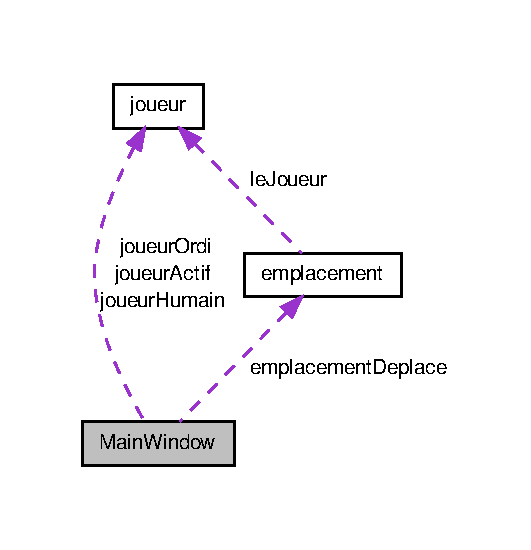
\includegraphics[width=255pt]{class_main_window__coll__graph}
\end{center}
\end{figure}
\subsection*{Connecteurs publics}
\begin{DoxyCompactItemize}
\item 
bool \hyperlink{class_main_window_a4ae4ac96dbfdcb80facbf7da0ae3fb5e}{est\-Coince} (\hyperlink{classemplacement}{emplacement} $\ast$)
\begin{DoxyCompactList}\small\item\em bool \hyperlink{class_main_window_a4ae4ac96dbfdcb80facbf7da0ae3fb5e}{est\-Coince(emplacement$\ast$)} \end{DoxyCompactList}\item 
bool \hyperlink{class_main_window_ac3a2c00ad936408dce78d15697eeef24}{accessible} (\hyperlink{classemplacement}{emplacement} $\ast$e1, \hyperlink{classemplacement}{emplacement} $\ast$e2)
\begin{DoxyCompactList}\small\item\em bool \hyperlink{class_main_window_ac3a2c00ad936408dce78d15697eeef24}{accessible(emplacement$\ast$ e1,emplacement$\ast$ e2)} \end{DoxyCompactList}\item 
void \hyperlink{class_main_window_a8e9fb499b85eef1d31b4caedcdad3424}{set\-Curseur} (Q\-Cursor \&cuseur)
\begin{DoxyCompactList}\small\item\em void \hyperlink{class_main_window_a8e9fb499b85eef1d31b4caedcdad3424}{set\-Curseur(\-Q\-Cursor \& cuseur)} \end{DoxyCompactList}\end{DoxyCompactItemize}
\subsection*{Fonctions membres publiques}
\begin{DoxyCompactItemize}
\item 
\hyperlink{class_main_window_a8b244be8b7b7db1b08de2a2acb9409db}{Main\-Window} (Q\-Widget $\ast$parent=0)
\begin{DoxyCompactList}\small\item\em \hyperlink{class_main_window}{Main\-Window}. \end{DoxyCompactList}\item 
\hyperlink{class_main_window_ae98d00a93bc118200eeef9f9bba1dba7}{$\sim$\-Main\-Window} ()
\begin{DoxyCompactList}\small\item\em Le destructeur. \end{DoxyCompactList}\item 
bool \hyperlink{class_main_window_a6dc1f84d9bc6e8ab7f1bb6bc04e2db49}{ligne} (int no)
\begin{DoxyCompactList}\small\item\em bool \hyperlink{class_main_window_a6dc1f84d9bc6e8ab7f1bb6bc04e2db49}{ligne(int no)} \end{DoxyCompactList}\item 
bool \hyperlink{class_main_window_a85653198b42750c0f09876f0af3715d7}{col} (int no)
\begin{DoxyCompactList}\small\item\em bool \hyperlink{class_main_window_a85653198b42750c0f09876f0af3715d7}{col(int no)} \end{DoxyCompactList}\item 
bool \hyperlink{class_main_window_a7b80bba7c56fbcc016dbc004d208ec31}{diag} (int no)
\begin{DoxyCompactList}\small\item\em bool \hyperlink{class_main_window_a7b80bba7c56fbcc016dbc004d208ec31}{diag(int no)} \end{DoxyCompactList}\item 
void \hyperlink{class_main_window_a1eefa05031d74694e4249a8c68741122}{set\-Emplacement\-Deplace} (\hyperlink{classemplacement}{emplacement} $\ast$e)
\begin{DoxyCompactList}\small\item\em void \hyperlink{class_main_window_a1eefa05031d74694e4249a8c68741122}{set\-Emplacement\-Deplace(emplacement$\ast$ e)} \end{DoxyCompactList}\item 
void \hyperlink{class_main_window_a3ab75adb0221eb5e362f2070f71ebc22}{reset\-Curseur} ()
\begin{DoxyCompactList}\small\item\em void \hyperlink{class_main_window_a3ab75adb0221eb5e362f2070f71ebc22}{reset\-Curseur()}  remet le curseur normal \end{DoxyCompactList}\item 
bool \hyperlink{class_main_window_a1810f8a7d5a8497d738d909efca8947b}{deja\-Gagne} (\hyperlink{classjoueur}{joueur} $\ast$un\-Joueur)
\begin{DoxyCompactList}\small\item\em bool \hyperlink{class_main_window_a1810f8a7d5a8497d738d909efca8947b}{deja\-Gagne(joueur $\ast$ un\-Joueur)} \end{DoxyCompactList}\item 
void \hyperlink{class_main_window_a3c0bedf7eae76f0c5ca35bd16491b919}{changement} ()
\begin{DoxyCompactList}\small\item\em void \hyperlink{class_main_window_a3c0bedf7eae76f0c5ca35bd16491b919}{changement()}  change de joueur actif \end{DoxyCompactList}\end{DoxyCompactItemize}
\subsection*{Attributs publics}
\begin{DoxyCompactItemize}
\item 
\hyperlink{classjoueur}{joueur} $\ast$ \hyperlink{class_main_window_a267d43ab6a839ee5f91869efa84cf271}{joueur\-Actif}
\begin{DoxyCompactList}\small\item\em joueur joueur\-Actif  définie le joueur actif \end{DoxyCompactList}\item 
\hyperlink{classemplacement}{emplacement} $\ast$ \hyperlink{class_main_window_ad334c5c1d3c58a97eb424324b3c6225e}{emplacement\-Deplace}
\begin{DoxyCompactList}\small\item\em emplacement emplacement\-Deplace  l'emplacement du jeton déplacé \end{DoxyCompactList}\item 
\hyperlink{classjoueur}{joueur} $\ast$ \hyperlink{class_main_window_a5d1e13ecdb63fa88e114565df70613aa}{joueur\-Humain}
\begin{DoxyCompactList}\small\item\em joueur joueur\-Humain  création d'un joueur humain (joueur1) \end{DoxyCompactList}\item 
\hyperlink{classjoueur}{joueur} $\ast$ \hyperlink{class_main_window_a7ce2a641dae02c27242c9bca5ec2174f}{joueur\-Ordi}
\begin{DoxyCompactList}\small\item\em joueur joueur\-Ordi  création d'un joueur ordinateur (joueur2) \end{DoxyCompactList}\item 
Q\-Pixmap \hyperlink{class_main_window_a40ca81795033b7d295527bc860f716cf}{pixmap\-Empty\-Emplacement}
\begin{DoxyCompactList}\small\item\em Q\-Pixmap pixmap\-Empty\-Emplacement  définie les emplacement vide sur le plateau (image rond noir) \end{DoxyCompactList}\item 
bool \hyperlink{class_main_window_a00d26707b5d27cc6ce07479a46244692}{partie\-Terminee}
\begin{DoxyCompactList}\small\item\em bool partie\-Terminee  renvoie vrai quand une partie est terminée \end{DoxyCompactList}\item 
Q\-Timer $\ast$ \hyperlink{class_main_window_a6d86dd50bcd7dc534fbc9fd374260554}{timer\-Tour}
\begin{DoxyCompactList}\small\item\em timer\-Tour  temps du tour, 30 secondes par tour par personne \end{DoxyCompactList}\end{DoxyCompactItemize}


\subsection{Description détaillée}
The \hyperlink{class_main_window}{Main\-Window} class. 

Définition à la ligne 26 du fichier mainwindow.\-h.



\subsection{Documentation des constructeurs et destructeur}
\hypertarget{class_main_window_a8b244be8b7b7db1b08de2a2acb9409db}{\index{Main\-Window@{Main\-Window}!Main\-Window@{Main\-Window}}
\index{Main\-Window@{Main\-Window}!MainWindow@{Main\-Window}}
\subsubsection[{Main\-Window}]{\setlength{\rightskip}{0pt plus 5cm}Main\-Window\-::\-Main\-Window (
\begin{DoxyParamCaption}
\item[{Q\-Widget $\ast$}]{parent = {\ttfamily 0}}
\end{DoxyParamCaption}
)\hspace{0.3cm}{\ttfamily [explicit]}}}\label{class_main_window_a8b244be8b7b7db1b08de2a2acb9409db}


\hyperlink{class_main_window}{Main\-Window}. 


\begin{DoxyParams}{Paramètres}
{\em parent} & \\
\hline
\end{DoxyParams}


Définition à la ligne 11 du fichier mainwindow.\-cpp.

\hypertarget{class_main_window_ae98d00a93bc118200eeef9f9bba1dba7}{\index{Main\-Window@{Main\-Window}!$\sim$\-Main\-Window@{$\sim$\-Main\-Window}}
\index{$\sim$\-Main\-Window@{$\sim$\-Main\-Window}!MainWindow@{Main\-Window}}
\subsubsection[{$\sim$\-Main\-Window}]{\setlength{\rightskip}{0pt plus 5cm}Main\-Window\-::$\sim$\-Main\-Window (
\begin{DoxyParamCaption}
{}
\end{DoxyParamCaption}
)}}\label{class_main_window_ae98d00a93bc118200eeef9f9bba1dba7}


Le destructeur. 

Le destructeur détruit l'instance et libère la mémoire allouée dynamiquement 

Définition à la ligne 60 du fichier mainwindow.\-cpp.



\subsection{Documentation des fonctions membres}
\hypertarget{class_main_window_ac3a2c00ad936408dce78d15697eeef24}{\index{Main\-Window@{Main\-Window}!accessible@{accessible}}
\index{accessible@{accessible}!MainWindow@{Main\-Window}}
\subsubsection[{accessible}]{\setlength{\rightskip}{0pt plus 5cm}bool Main\-Window\-::accessible (
\begin{DoxyParamCaption}
\item[{{\bf emplacement} $\ast$}]{e1, }
\item[{{\bf emplacement} $\ast$}]{e2}
\end{DoxyParamCaption}
)\hspace{0.3cm}{\ttfamily [slot]}}}\label{class_main_window_ac3a2c00ad936408dce78d15697eeef24}


bool \hyperlink{class_main_window_ac3a2c00ad936408dce78d15697eeef24}{accessible(emplacement$\ast$ e1,emplacement$\ast$ e2)} 


\begin{DoxyParams}{Paramètres}
{\em e1} & \-: emplacement inital du jeton \\
\hline
{\em e2} & \-: emplacement destination du jeton \\
\hline
\end{DoxyParams}
\begin{DoxyReturn}{Renvoie}
renvoie vrai si l'emplacement (e2) est accessible pour le jeton selectionné qui était en (e1) 
\end{DoxyReturn}


Définition à la ligne 130 du fichier mainwindow.\-cpp.

\hypertarget{class_main_window_a3c0bedf7eae76f0c5ca35bd16491b919}{\index{Main\-Window@{Main\-Window}!changement@{changement}}
\index{changement@{changement}!MainWindow@{Main\-Window}}
\subsubsection[{changement}]{\setlength{\rightskip}{0pt plus 5cm}void Main\-Window\-::changement (
\begin{DoxyParamCaption}
{}
\end{DoxyParamCaption}
)}}\label{class_main_window_a3c0bedf7eae76f0c5ca35bd16491b919}


void \hyperlink{class_main_window_a3c0bedf7eae76f0c5ca35bd16491b919}{changement()}  change de joueur actif 



Définition à la ligne 107 du fichier mainwindow.\-cpp.

\hypertarget{class_main_window_a85653198b42750c0f09876f0af3715d7}{\index{Main\-Window@{Main\-Window}!col@{col}}
\index{col@{col}!MainWindow@{Main\-Window}}
\subsubsection[{col}]{\setlength{\rightskip}{0pt plus 5cm}bool Main\-Window\-::col (
\begin{DoxyParamCaption}
\item[{int}]{no}
\end{DoxyParamCaption}
)}}\label{class_main_window_a85653198b42750c0f09876f0af3715d7}


bool \hyperlink{class_main_window_a85653198b42750c0f09876f0af3715d7}{col(int no)} 


\begin{DoxyParams}{Paramètres}
{\em int} & no \\
\hline
\end{DoxyParams}
\begin{DoxyReturn}{Renvoie}
retourne vrai si la col no est pleine  colonne sur le plateau de jeu 
\end{DoxyReturn}


Définition à la ligne 79 du fichier mainwindow.\-cpp.

\hypertarget{class_main_window_a1810f8a7d5a8497d738d909efca8947b}{\index{Main\-Window@{Main\-Window}!deja\-Gagne@{deja\-Gagne}}
\index{deja\-Gagne@{deja\-Gagne}!MainWindow@{Main\-Window}}
\subsubsection[{deja\-Gagne}]{\setlength{\rightskip}{0pt plus 5cm}bool Main\-Window\-::deja\-Gagne (
\begin{DoxyParamCaption}
\item[{{\bf joueur} $\ast$}]{un\-Joueur}
\end{DoxyParamCaption}
)}}\label{class_main_window_a1810f8a7d5a8497d738d909efca8947b}


bool \hyperlink{class_main_window_a1810f8a7d5a8497d738d909efca8947b}{deja\-Gagne(joueur $\ast$ un\-Joueur)} 


\begin{DoxyParams}{Paramètres}
{\em un\-Joueur} & joueur$\ast$ \\
\hline
\end{DoxyParams}
\begin{DoxyReturn}{Renvoie}
renvoie vrai si un joueur a déjà gagné 
\end{DoxyReturn}


Définition à la ligne 93 du fichier mainwindow.\-cpp.

\hypertarget{class_main_window_a7b80bba7c56fbcc016dbc004d208ec31}{\index{Main\-Window@{Main\-Window}!diag@{diag}}
\index{diag@{diag}!MainWindow@{Main\-Window}}
\subsubsection[{diag}]{\setlength{\rightskip}{0pt plus 5cm}bool Main\-Window\-::diag (
\begin{DoxyParamCaption}
\item[{int}]{no}
\end{DoxyParamCaption}
)}}\label{class_main_window_a7b80bba7c56fbcc016dbc004d208ec31}


bool \hyperlink{class_main_window_a7b80bba7c56fbcc016dbc004d208ec31}{diag(int no)} 


\begin{DoxyParams}{Paramètres}
{\em int} & no \\
\hline
\end{DoxyParams}
\begin{DoxyReturn}{Renvoie}
retourne vrai si la diag no est pleine  diagonal sur le plateau de jeu 
\end{DoxyReturn}


Définition à la ligne 86 du fichier mainwindow.\-cpp.

\hypertarget{class_main_window_a4ae4ac96dbfdcb80facbf7da0ae3fb5e}{\index{Main\-Window@{Main\-Window}!est\-Coince@{est\-Coince}}
\index{est\-Coince@{est\-Coince}!MainWindow@{Main\-Window}}
\subsubsection[{est\-Coince}]{\setlength{\rightskip}{0pt plus 5cm}bool Main\-Window\-::est\-Coince (
\begin{DoxyParamCaption}
\item[{{\bf emplacement} $\ast$}]{}
\end{DoxyParamCaption}
)\hspace{0.3cm}{\ttfamily [slot]}}}\label{class_main_window_a4ae4ac96dbfdcb80facbf7da0ae3fb5e}


bool \hyperlink{class_main_window_a4ae4ac96dbfdcb80facbf7da0ae3fb5e}{est\-Coince(emplacement$\ast$)} 


\begin{DoxyParams}{Paramètres}
{\em emplacement$\ast$} & l'emplacement du jeton selectionné \\
\hline
\end{DoxyParams}
\begin{DoxyReturn}{Renvoie}
renvoie faux 
\end{DoxyReturn}


Définition à la ligne 125 du fichier mainwindow.\-cpp.

\hypertarget{class_main_window_a6dc1f84d9bc6e8ab7f1bb6bc04e2db49}{\index{Main\-Window@{Main\-Window}!ligne@{ligne}}
\index{ligne@{ligne}!MainWindow@{Main\-Window}}
\subsubsection[{ligne}]{\setlength{\rightskip}{0pt plus 5cm}bool Main\-Window\-::ligne (
\begin{DoxyParamCaption}
\item[{int}]{no}
\end{DoxyParamCaption}
)}}\label{class_main_window_a6dc1f84d9bc6e8ab7f1bb6bc04e2db49}


bool \hyperlink{class_main_window_a6dc1f84d9bc6e8ab7f1bb6bc04e2db49}{ligne(int no)} 


\begin{DoxyParams}{Paramètres}
{\em int} & no \\
\hline
\end{DoxyParams}
\begin{DoxyReturn}{Renvoie}
retourne vrai si la ligne no est pleine  ligne sur le plateau de jeu 
\end{DoxyReturn}


Définition à la ligne 72 du fichier mainwindow.\-cpp.

\hypertarget{class_main_window_a3ab75adb0221eb5e362f2070f71ebc22}{\index{Main\-Window@{Main\-Window}!reset\-Curseur@{reset\-Curseur}}
\index{reset\-Curseur@{reset\-Curseur}!MainWindow@{Main\-Window}}
\subsubsection[{reset\-Curseur}]{\setlength{\rightskip}{0pt plus 5cm}void Main\-Window\-::reset\-Curseur (
\begin{DoxyParamCaption}
{}
\end{DoxyParamCaption}
)}}\label{class_main_window_a3ab75adb0221eb5e362f2070f71ebc22}


void \hyperlink{class_main_window_a3ab75adb0221eb5e362f2070f71ebc22}{reset\-Curseur()}  remet le curseur normal 



Définition à la ligne 55 du fichier mainwindow.\-cpp.

\hypertarget{class_main_window_a8e9fb499b85eef1d31b4caedcdad3424}{\index{Main\-Window@{Main\-Window}!set\-Curseur@{set\-Curseur}}
\index{set\-Curseur@{set\-Curseur}!MainWindow@{Main\-Window}}
\subsubsection[{set\-Curseur}]{\setlength{\rightskip}{0pt plus 5cm}void Main\-Window\-::set\-Curseur (
\begin{DoxyParamCaption}
\item[{Q\-Cursor \&}]{cuseur}
\end{DoxyParamCaption}
)\hspace{0.3cm}{\ttfamily [slot]}}}\label{class_main_window_a8e9fb499b85eef1d31b4caedcdad3424}


void \hyperlink{class_main_window_a8e9fb499b85eef1d31b4caedcdad3424}{set\-Curseur(\-Q\-Cursor \& cuseur)} 


\begin{DoxyParams}{Paramètres}
{\em Q\-Cursor} & cuseur \\
\hline
\end{DoxyParams}


Définition à la ligne 48 du fichier mainwindow.\-cpp.

\hypertarget{class_main_window_a1eefa05031d74694e4249a8c68741122}{\index{Main\-Window@{Main\-Window}!set\-Emplacement\-Deplace@{set\-Emplacement\-Deplace}}
\index{set\-Emplacement\-Deplace@{set\-Emplacement\-Deplace}!MainWindow@{Main\-Window}}
\subsubsection[{set\-Emplacement\-Deplace}]{\setlength{\rightskip}{0pt plus 5cm}void Main\-Window\-::set\-Emplacement\-Deplace (
\begin{DoxyParamCaption}
\item[{{\bf emplacement} $\ast$}]{e}
\end{DoxyParamCaption}
)\hspace{0.3cm}{\ttfamily [inline]}}}\label{class_main_window_a1eefa05031d74694e4249a8c68741122}


void \hyperlink{class_main_window_a1eefa05031d74694e4249a8c68741122}{set\-Emplacement\-Deplace(emplacement$\ast$ e)} 


\begin{DoxyParams}{Paramètres}
{\em emplacement} & e  emplacement\-Deplace prendre la valeur de l'emplacement e \\
\hline
\end{DoxyParams}


Définition à la ligne 82 du fichier mainwindow.\-h.



\subsection{Documentation des données membres}
\hypertarget{class_main_window_ad334c5c1d3c58a97eb424324b3c6225e}{\index{Main\-Window@{Main\-Window}!emplacement\-Deplace@{emplacement\-Deplace}}
\index{emplacement\-Deplace@{emplacement\-Deplace}!MainWindow@{Main\-Window}}
\subsubsection[{emplacement\-Deplace}]{\setlength{\rightskip}{0pt plus 5cm}{\bf emplacement} $\ast$ Main\-Window\-::emplacement\-Deplace}}\label{class_main_window_ad334c5c1d3c58a97eb424324b3c6225e}


emplacement emplacement\-Deplace  l'emplacement du jeton déplacé 



Définition à la ligne 76 du fichier mainwindow.\-h.

\hypertarget{class_main_window_a267d43ab6a839ee5f91869efa84cf271}{\index{Main\-Window@{Main\-Window}!joueur\-Actif@{joueur\-Actif}}
\index{joueur\-Actif@{joueur\-Actif}!MainWindow@{Main\-Window}}
\subsubsection[{joueur\-Actif}]{\setlength{\rightskip}{0pt plus 5cm}{\bf joueur} $\ast$ Main\-Window\-::joueur\-Actif}}\label{class_main_window_a267d43ab6a839ee5f91869efa84cf271}


joueur joueur\-Actif  définie le joueur actif 



Définition à la ligne 49 du fichier mainwindow.\-h.

\hypertarget{class_main_window_a5d1e13ecdb63fa88e114565df70613aa}{\index{Main\-Window@{Main\-Window}!joueur\-Humain@{joueur\-Humain}}
\index{joueur\-Humain@{joueur\-Humain}!MainWindow@{Main\-Window}}
\subsubsection[{joueur\-Humain}]{\setlength{\rightskip}{0pt plus 5cm}{\bf joueur} $\ast$ Main\-Window\-::joueur\-Humain}}\label{class_main_window_a5d1e13ecdb63fa88e114565df70613aa}


joueur joueur\-Humain  création d'un joueur humain (joueur1) 



Définition à la ligne 104 du fichier mainwindow.\-h.

\hypertarget{class_main_window_a7ce2a641dae02c27242c9bca5ec2174f}{\index{Main\-Window@{Main\-Window}!joueur\-Ordi@{joueur\-Ordi}}
\index{joueur\-Ordi@{joueur\-Ordi}!MainWindow@{Main\-Window}}
\subsubsection[{joueur\-Ordi}]{\setlength{\rightskip}{0pt plus 5cm}{\bf joueur} $\ast$ Main\-Window\-::joueur\-Ordi}}\label{class_main_window_a7ce2a641dae02c27242c9bca5ec2174f}


joueur joueur\-Ordi  création d'un joueur ordinateur (joueur2) 



Définition à la ligne 110 du fichier mainwindow.\-h.

\hypertarget{class_main_window_a00d26707b5d27cc6ce07479a46244692}{\index{Main\-Window@{Main\-Window}!partie\-Terminee@{partie\-Terminee}}
\index{partie\-Terminee@{partie\-Terminee}!MainWindow@{Main\-Window}}
\subsubsection[{partie\-Terminee}]{\setlength{\rightskip}{0pt plus 5cm}bool Main\-Window\-::partie\-Terminee}}\label{class_main_window_a00d26707b5d27cc6ce07479a46244692}


bool partie\-Terminee  renvoie vrai quand une partie est terminée 



Définition à la ligne 121 du fichier mainwindow.\-h.

\hypertarget{class_main_window_a40ca81795033b7d295527bc860f716cf}{\index{Main\-Window@{Main\-Window}!pixmap\-Empty\-Emplacement@{pixmap\-Empty\-Emplacement}}
\index{pixmap\-Empty\-Emplacement@{pixmap\-Empty\-Emplacement}!MainWindow@{Main\-Window}}
\subsubsection[{pixmap\-Empty\-Emplacement}]{\setlength{\rightskip}{0pt plus 5cm}Q\-Pixmap Main\-Window\-::pixmap\-Empty\-Emplacement}}\label{class_main_window_a40ca81795033b7d295527bc860f716cf}


Q\-Pixmap pixmap\-Empty\-Emplacement  définie les emplacement vide sur le plateau (image rond noir) 



Définition à la ligne 116 du fichier mainwindow.\-h.

\hypertarget{class_main_window_a6d86dd50bcd7dc534fbc9fd374260554}{\index{Main\-Window@{Main\-Window}!timer\-Tour@{timer\-Tour}}
\index{timer\-Tour@{timer\-Tour}!MainWindow@{Main\-Window}}
\subsubsection[{timer\-Tour}]{\setlength{\rightskip}{0pt plus 5cm}Q\-Timer $\ast$ Main\-Window\-::timer\-Tour}}\label{class_main_window_a6d86dd50bcd7dc534fbc9fd374260554}


timer\-Tour  temps du tour, 30 secondes par tour par personne 



Définition à la ligne 127 du fichier mainwindow.\-h.



La documentation de cette classe a été générée à partir des fichiers suivants \-:\begin{DoxyCompactItemize}
\item 
\hyperlink{mainwindow_8h}{mainwindow.\-h}\item 
\hyperlink{mainwindow_8cpp}{mainwindow.\-cpp}\end{DoxyCompactItemize}

\hypertarget{classorg_1_1qtproject_1_1qt5_1_1android_1_1bindings_1_1_qt_activity}{\section{Référence de la classe org.\-qtproject.\-qt5.\-android.\-bindings.\-Qt\-Activity}
\label{classorg_1_1qtproject_1_1qt5_1_1android_1_1bindings_1_1_qt_activity}\index{org.\-qtproject.\-qt5.\-android.\-bindings.\-Qt\-Activity@{org.\-qtproject.\-qt5.\-android.\-bindings.\-Qt\-Activity}}
}


Graphe d'héritage de org.\-qtproject.\-qt5.\-android.\-bindings.\-Qt\-Activity\-:\nopagebreak
\begin{figure}[H]
\begin{center}
\leavevmode
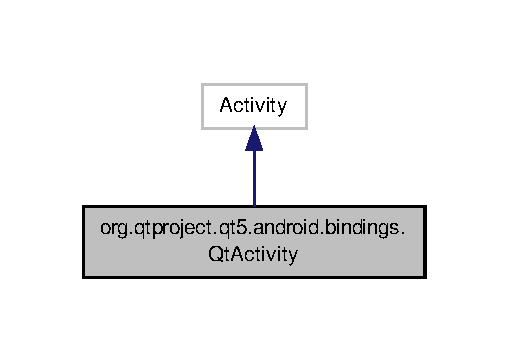
\includegraphics[width=244pt]{classorg_1_1qtproject_1_1qt5_1_1android_1_1bindings_1_1_qt_activity__inherit__graph}
\end{center}
\end{figure}


Graphe de collaboration de org.\-qtproject.\-qt5.\-android.\-bindings.\-Qt\-Activity\-:\nopagebreak
\begin{figure}[H]
\begin{center}
\leavevmode
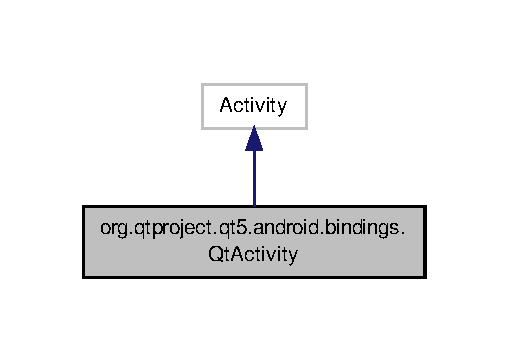
\includegraphics[width=244pt]{classorg_1_1qtproject_1_1qt5_1_1android_1_1bindings_1_1_qt_activity__coll__graph}
\end{center}
\end{figure}
\subsection*{Fonctions membres publiques}
\begin{DoxyCompactItemize}
\item 
boolean \hyperlink{classorg_1_1qtproject_1_1qt5_1_1android_1_1bindings_1_1_qt_activity_a3419f10b60670ae0fd0a222fcd684273}{dispatch\-Key\-Event} (Key\-Event event)
\item 
boolean \hyperlink{classorg_1_1qtproject_1_1qt5_1_1android_1_1bindings_1_1_qt_activity_a0222dd1edd412d5573914d8e563d8dfc}{super\-\_\-dispatch\-Key\-Event} (Key\-Event event)
\item 
boolean \hyperlink{classorg_1_1qtproject_1_1qt5_1_1android_1_1bindings_1_1_qt_activity_a7eacf9d228567bace814d7d90cc88dc1}{dispatch\-Populate\-Accessibility\-Event} (Accessibility\-Event event)
\item 
boolean \hyperlink{classorg_1_1qtproject_1_1qt5_1_1android_1_1bindings_1_1_qt_activity_a174082c8c4aa301a2a8c78ce237bca22}{super\-\_\-dispatch\-Populate\-Accessibility\-Event} (Accessibility\-Event event)
\item 
boolean \hyperlink{classorg_1_1qtproject_1_1qt5_1_1android_1_1bindings_1_1_qt_activity_a080d702cac33de4a97b4645567cf8c04}{dispatch\-Touch\-Event} (Motion\-Event ev)
\item 
boolean \hyperlink{classorg_1_1qtproject_1_1qt5_1_1android_1_1bindings_1_1_qt_activity_a8525630fd66e1d88e94f7bc9457bbd1b}{super\-\_\-dispatch\-Touch\-Event} (Motion\-Event event)
\item 
boolean \hyperlink{classorg_1_1qtproject_1_1qt5_1_1android_1_1bindings_1_1_qt_activity_ad305b6d78907e6fc4bc4fa9b77256a22}{dispatch\-Trackball\-Event} (Motion\-Event ev)
\item 
boolean \hyperlink{classorg_1_1qtproject_1_1qt5_1_1android_1_1bindings_1_1_qt_activity_a84a82b3eb7dd352d126c55272c64264a}{super\-\_\-dispatch\-Trackball\-Event} (Motion\-Event event)
\item 
void \hyperlink{classorg_1_1qtproject_1_1qt5_1_1android_1_1bindings_1_1_qt_activity_a03bf6f3f50c07592cbee97ce9ebdb315}{super\-\_\-on\-Activity\-Result} (int request\-Code, int result\-Code, Intent data)
\item 
void \hyperlink{classorg_1_1qtproject_1_1qt5_1_1android_1_1bindings_1_1_qt_activity_a03b4db053b9528617c37bab2d47fc803}{super\-\_\-on\-Apply\-Theme\-Resource} (Theme theme, int resid, boolean first)
\item 
void \hyperlink{classorg_1_1qtproject_1_1qt5_1_1android_1_1bindings_1_1_qt_activity_ac369eb38a2ea1f7a0d61c44a30d63620}{super\-\_\-on\-Child\-Title\-Changed} (Activity child\-Activity, Char\-Sequence title)
\item 
void \hyperlink{classorg_1_1qtproject_1_1qt5_1_1android_1_1bindings_1_1_qt_activity_a75ef70261caa7d4db3041147dc46c5d0}{on\-Configuration\-Changed} (Configuration new\-Config)
\item 
void \hyperlink{classorg_1_1qtproject_1_1qt5_1_1android_1_1bindings_1_1_qt_activity_a1c7f2e1b1ce16f2bfa70f38d88740565}{super\-\_\-on\-Configuration\-Changed} (Configuration new\-Config)
\item 
void \hyperlink{classorg_1_1qtproject_1_1qt5_1_1android_1_1bindings_1_1_qt_activity_a6310ffd404267a66b52dd4c3b357b560}{on\-Content\-Changed} ()
\item 
void \hyperlink{classorg_1_1qtproject_1_1qt5_1_1android_1_1bindings_1_1_qt_activity_a65dc57b70d42eb56f6bc12f7e0c49022}{super\-\_\-on\-Content\-Changed} ()
\item 
boolean \hyperlink{classorg_1_1qtproject_1_1qt5_1_1android_1_1bindings_1_1_qt_activity_a67108692da62e48e5d02b22ed3d83769}{on\-Context\-Item\-Selected} (Menu\-Item item)
\item 
boolean \hyperlink{classorg_1_1qtproject_1_1qt5_1_1android_1_1bindings_1_1_qt_activity_a7281a498436213e739110753b357c0bd}{super\-\_\-on\-Context\-Item\-Selected} (Menu\-Item item)
\item 
void \hyperlink{classorg_1_1qtproject_1_1qt5_1_1android_1_1bindings_1_1_qt_activity_a3e845800dc8fc21ff23589005d1a781c}{on\-Context\-Menu\-Closed} (Menu menu)
\item 
void \hyperlink{classorg_1_1qtproject_1_1qt5_1_1android_1_1bindings_1_1_qt_activity_a1b845060cb1ae8dde9bb8a60339b9468}{super\-\_\-on\-Context\-Menu\-Closed} (Menu menu)
\item 
void \hyperlink{classorg_1_1qtproject_1_1qt5_1_1android_1_1bindings_1_1_qt_activity_aa826639406d6f0697e0f1afcf69c748c}{on\-Create} (Bundle saved\-Instance\-State)
\item 
void \hyperlink{classorg_1_1qtproject_1_1qt5_1_1android_1_1bindings_1_1_qt_activity_a924489f96650a755cf63980f3d388e8e}{on\-Create\-Context\-Menu} (Context\-Menu menu, View v, Context\-Menu\-Info menu\-Info)
\item 
void \hyperlink{classorg_1_1qtproject_1_1qt5_1_1android_1_1bindings_1_1_qt_activity_ae235bff28fac3ae862e49a1fc52caf15}{super\-\_\-on\-Create\-Context\-Menu} (Context\-Menu menu, View v, Context\-Menu\-Info menu\-Info)
\item 
Char\-Sequence \hyperlink{classorg_1_1qtproject_1_1qt5_1_1android_1_1bindings_1_1_qt_activity_af86865337837c2c780913132b7118d69}{on\-Create\-Description} ()
\item 
Char\-Sequence \hyperlink{classorg_1_1qtproject_1_1qt5_1_1android_1_1bindings_1_1_qt_activity_a213a5e7065a1b53244d8b3642a23b2e4}{super\-\_\-on\-Create\-Description} ()
\item 
Dialog \hyperlink{classorg_1_1qtproject_1_1qt5_1_1android_1_1bindings_1_1_qt_activity_a946099e0315e24f0c40338b69e0d1cdf}{super\-\_\-on\-Create\-Dialog} (int id)
\item 
boolean \hyperlink{classorg_1_1qtproject_1_1qt5_1_1android_1_1bindings_1_1_qt_activity_a9303a2dd16e8deb7cdcf143ae6b480f4}{on\-Create\-Options\-Menu} (Menu menu)
\item 
boolean \hyperlink{classorg_1_1qtproject_1_1qt5_1_1android_1_1bindings_1_1_qt_activity_a25d0cb2383a485b28f53026ebe050dd4}{super\-\_\-on\-Create\-Options\-Menu} (Menu menu)
\item 
boolean \hyperlink{classorg_1_1qtproject_1_1qt5_1_1android_1_1bindings_1_1_qt_activity_a617b7c2c432bc9894d3c0b2490d27b41}{on\-Create\-Panel\-Menu} (int feature\-Id, Menu menu)
\item 
boolean \hyperlink{classorg_1_1qtproject_1_1qt5_1_1android_1_1bindings_1_1_qt_activity_a3d105b186ba9bf7d089699dbd5ca3c45}{super\-\_\-on\-Create\-Panel\-Menu} (int feature\-Id, Menu menu)
\item 
View \hyperlink{classorg_1_1qtproject_1_1qt5_1_1android_1_1bindings_1_1_qt_activity_aefde1977c2ccae37e5f1a927f7e9e9ee}{on\-Create\-Panel\-View} (int feature\-Id)
\item 
View \hyperlink{classorg_1_1qtproject_1_1qt5_1_1android_1_1bindings_1_1_qt_activity_ab37f48e1ce50767f29be1cebd4fc96e0}{super\-\_\-on\-Create\-Panel\-View} (int feature\-Id)
\item 
boolean \hyperlink{classorg_1_1qtproject_1_1qt5_1_1android_1_1bindings_1_1_qt_activity_a961e15fb9b7bcdc7e4310e881656e1d7}{on\-Create\-Thumbnail} (Bitmap out\-Bitmap, Canvas canvas)
\item 
boolean \hyperlink{classorg_1_1qtproject_1_1qt5_1_1android_1_1bindings_1_1_qt_activity_a2af36b766142fa45fa77623e549112ac}{super\-\_\-on\-Create\-Thumbnail} (Bitmap out\-Bitmap, Canvas canvas)
\item 
View \hyperlink{classorg_1_1qtproject_1_1qt5_1_1android_1_1bindings_1_1_qt_activity_a4f26e1f33245742068eb9b79689f69e5}{on\-Create\-View} (String name, Context context, Attribute\-Set attrs)
\item 
View \hyperlink{classorg_1_1qtproject_1_1qt5_1_1android_1_1bindings_1_1_qt_activity_a4e054eb047b9531cc8abaa75039136f2}{super\-\_\-on\-Create\-View} (String name, Context context, Attribute\-Set attrs)
\item 
boolean \hyperlink{classorg_1_1qtproject_1_1qt5_1_1android_1_1bindings_1_1_qt_activity_ac1ee5a8d6b1ed5e7757139be8d7810be}{on\-Key\-Down} (int key\-Code, Key\-Event event)
\item 
boolean \hyperlink{classorg_1_1qtproject_1_1qt5_1_1android_1_1bindings_1_1_qt_activity_af7fbc3d78f28c7599fac81499717ac8d}{super\-\_\-on\-Key\-Down} (int key\-Code, Key\-Event event)
\item 
boolean \hyperlink{classorg_1_1qtproject_1_1qt5_1_1android_1_1bindings_1_1_qt_activity_a9b41df58aada132667b9af5a8aa01aa7}{on\-Key\-Multiple} (int key\-Code, int repeat\-Count, Key\-Event event)
\item 
boolean \hyperlink{classorg_1_1qtproject_1_1qt5_1_1android_1_1bindings_1_1_qt_activity_a108ba4840f9990f299beb44cced0a45d}{super\-\_\-on\-Key\-Multiple} (int key\-Code, int repeat\-Count, Key\-Event event)
\item 
boolean \hyperlink{classorg_1_1qtproject_1_1qt5_1_1android_1_1bindings_1_1_qt_activity_ac81bcf0a973ed2f8035bc3af8ee73f78}{on\-Key\-Up} (int key\-Code, Key\-Event event)
\item 
boolean \hyperlink{classorg_1_1qtproject_1_1qt5_1_1android_1_1bindings_1_1_qt_activity_a0e236df83e1edd02ba8587199fc47e05}{super\-\_\-on\-Key\-Up} (int key\-Code, Key\-Event event)
\item 
void \hyperlink{classorg_1_1qtproject_1_1qt5_1_1android_1_1bindings_1_1_qt_activity_a60dde1c5c76102c0514119fbc9515450}{on\-Low\-Memory} ()
\item 
boolean \hyperlink{classorg_1_1qtproject_1_1qt5_1_1android_1_1bindings_1_1_qt_activity_a15f3f492aba46975a36f1ebdfbe5ba45}{on\-Menu\-Item\-Selected} (int feature\-Id, Menu\-Item item)
\item 
boolean \hyperlink{classorg_1_1qtproject_1_1qt5_1_1android_1_1bindings_1_1_qt_activity_a054b8b51a53012f32a3d30bf395c18ca}{super\-\_\-on\-Menu\-Item\-Selected} (int feature\-Id, Menu\-Item item)
\item 
boolean \hyperlink{classorg_1_1qtproject_1_1qt5_1_1android_1_1bindings_1_1_qt_activity_afa718d6a5777a519b1d513d7cbda938a}{on\-Menu\-Opened} (int feature\-Id, Menu menu)
\item 
boolean \hyperlink{classorg_1_1qtproject_1_1qt5_1_1android_1_1bindings_1_1_qt_activity_ab1719c7260a5641289249620984077bd}{super\-\_\-on\-Menu\-Opened} (int feature\-Id, Menu menu)
\item 
void \hyperlink{classorg_1_1qtproject_1_1qt5_1_1android_1_1bindings_1_1_qt_activity_afb8a02b6c2e3c8e868f8cce113f50b18}{super\-\_\-on\-New\-Intent} (Intent intent)
\item 
boolean \hyperlink{classorg_1_1qtproject_1_1qt5_1_1android_1_1bindings_1_1_qt_activity_a1062f0dfba41ba945835041b94bfe4fa}{on\-Options\-Item\-Selected} (Menu\-Item item)
\item 
boolean \hyperlink{classorg_1_1qtproject_1_1qt5_1_1android_1_1bindings_1_1_qt_activity_aab1ebb0d4fe4429af0b9e79a4a6295ad}{super\-\_\-on\-Options\-Item\-Selected} (Menu\-Item item)
\item 
void \hyperlink{classorg_1_1qtproject_1_1qt5_1_1android_1_1bindings_1_1_qt_activity_aad115f4cdaebb71916b85ac6309a83c4}{on\-Options\-Menu\-Closed} (Menu menu)
\item 
void \hyperlink{classorg_1_1qtproject_1_1qt5_1_1android_1_1bindings_1_1_qt_activity_abd8ef4d5f57f3046c3065cbe806f690b}{super\-\_\-on\-Options\-Menu\-Closed} (Menu menu)
\item 
void \hyperlink{classorg_1_1qtproject_1_1qt5_1_1android_1_1bindings_1_1_qt_activity_a2b39eac5b8b7003b20171ddce6b16e37}{on\-Panel\-Closed} (int feature\-Id, Menu menu)
\item 
void \hyperlink{classorg_1_1qtproject_1_1qt5_1_1android_1_1bindings_1_1_qt_activity_a5f9ad8da2fcebff92ef8c86583091d75}{super\-\_\-on\-Panel\-Closed} (int feature\-Id, Menu menu)
\item 
void \hyperlink{classorg_1_1qtproject_1_1qt5_1_1android_1_1bindings_1_1_qt_activity_aacc652635f4bf45e2fa182dc44e8df13}{super\-\_\-on\-Prepare\-Dialog} (int id, Dialog dialog)
\item 
boolean \hyperlink{classorg_1_1qtproject_1_1qt5_1_1android_1_1bindings_1_1_qt_activity_a71a7e747de798c51b6a385b5e8a99c61}{on\-Prepare\-Options\-Menu} (Menu menu)
\item 
boolean \hyperlink{classorg_1_1qtproject_1_1qt5_1_1android_1_1bindings_1_1_qt_activity_a9f7f63be6b9a75253b784e80bfa74f69}{super\-\_\-on\-Prepare\-Options\-Menu} (Menu menu)
\item 
boolean \hyperlink{classorg_1_1qtproject_1_1qt5_1_1android_1_1bindings_1_1_qt_activity_a668c15554849a0bce9422eb709b5cacc}{on\-Prepare\-Panel} (int feature\-Id, View view, Menu menu)
\item 
boolean \hyperlink{classorg_1_1qtproject_1_1qt5_1_1android_1_1bindings_1_1_qt_activity_ab8af6f3b5a5b4547829dc68e7c31fd86}{super\-\_\-on\-Prepare\-Panel} (int feature\-Id, View view, Menu menu)
\item 
void \hyperlink{classorg_1_1qtproject_1_1qt5_1_1android_1_1bindings_1_1_qt_activity_a73303f1db92072963fe8592eb05b0258}{super\-\_\-on\-Restore\-Instance\-State} (Bundle saved\-Instance\-State)
\item 
Object \hyperlink{classorg_1_1qtproject_1_1qt5_1_1android_1_1bindings_1_1_qt_activity_a5954d45f88dd09deba757e671de9077d}{on\-Retain\-Non\-Configuration\-Instance} ()
\item 
Object \hyperlink{classorg_1_1qtproject_1_1qt5_1_1android_1_1bindings_1_1_qt_activity_a4fa6ba75523273de5b492052f1ae06f0}{super\-\_\-on\-Retain\-Non\-Configuration\-Instance} ()
\item 
void \hyperlink{classorg_1_1qtproject_1_1qt5_1_1android_1_1bindings_1_1_qt_activity_a8fb26c42bd8d7516bf863cc5fb50e287}{super\-\_\-on\-Save\-Instance\-State} (Bundle out\-State)
\item 
boolean \hyperlink{classorg_1_1qtproject_1_1qt5_1_1android_1_1bindings_1_1_qt_activity_aa1c033b0b0bbc4cb9c193b239992fcb8}{on\-Search\-Requested} ()
\item 
boolean \hyperlink{classorg_1_1qtproject_1_1qt5_1_1android_1_1bindings_1_1_qt_activity_a41f90d68a12b8140f7b0f4c4037c2567}{super\-\_\-on\-Search\-Requested} ()
\item 
void \hyperlink{classorg_1_1qtproject_1_1qt5_1_1android_1_1bindings_1_1_qt_activity_aa3982942fa042ca69a13ffbaff0ef403}{super\-\_\-on\-Title\-Changed} (Char\-Sequence title, int color)
\item 
boolean \hyperlink{classorg_1_1qtproject_1_1qt5_1_1android_1_1bindings_1_1_qt_activity_ada200302a153c7dbab3e55b746a7a179}{on\-Touch\-Event} (Motion\-Event event)
\item 
boolean \hyperlink{classorg_1_1qtproject_1_1qt5_1_1android_1_1bindings_1_1_qt_activity_a216ec445b2cc31beac2032e38dd5e949}{super\-\_\-on\-Touch\-Event} (Motion\-Event event)
\item 
boolean \hyperlink{classorg_1_1qtproject_1_1qt5_1_1android_1_1bindings_1_1_qt_activity_a27faf58c38193faea2782ff85cedb567}{on\-Trackball\-Event} (Motion\-Event event)
\item 
boolean \hyperlink{classorg_1_1qtproject_1_1qt5_1_1android_1_1bindings_1_1_qt_activity_a4ee363f63dfde917e450b70c8880fef9}{super\-\_\-on\-Trackball\-Event} (Motion\-Event event)
\item 
void \hyperlink{classorg_1_1qtproject_1_1qt5_1_1android_1_1bindings_1_1_qt_activity_a3917d7d3ac6ab5bf31444d31b2784828}{on\-User\-Interaction} ()
\item 
void \hyperlink{classorg_1_1qtproject_1_1qt5_1_1android_1_1bindings_1_1_qt_activity_a706d78309b31669959a98b46952de75c}{super\-\_\-on\-User\-Interaction} ()
\item 
void \hyperlink{classorg_1_1qtproject_1_1qt5_1_1android_1_1bindings_1_1_qt_activity_ae71ad183d13c1bbb1fd1dccee12dde24}{super\-\_\-on\-User\-Leave\-Hint} ()
\item 
void \hyperlink{classorg_1_1qtproject_1_1qt5_1_1android_1_1bindings_1_1_qt_activity_af881fa829fb552af632f8b1bba96f351}{on\-Window\-Attributes\-Changed} (Layout\-Params params)
\item 
void \hyperlink{classorg_1_1qtproject_1_1qt5_1_1android_1_1bindings_1_1_qt_activity_aa510558df5227f66d81d6119389e7886}{super\-\_\-on\-Window\-Attributes\-Changed} (Layout\-Params params)
\item 
void \hyperlink{classorg_1_1qtproject_1_1qt5_1_1android_1_1bindings_1_1_qt_activity_ab161d356ebf5044a00182ffaf79d3437}{on\-Window\-Focus\-Changed} (boolean has\-Focus)
\item 
void \hyperlink{classorg_1_1qtproject_1_1qt5_1_1android_1_1bindings_1_1_qt_activity_a3d01ed848c426f937fe18214ff006931}{super\-\_\-on\-Window\-Focus\-Changed} (boolean has\-Focus)
\item 
void \hyperlink{classorg_1_1qtproject_1_1qt5_1_1android_1_1bindings_1_1_qt_activity_a052fd4aee0de52bcf2d8a10c5671d586}{on\-Attached\-To\-Window} ()
\item 
void \hyperlink{classorg_1_1qtproject_1_1qt5_1_1android_1_1bindings_1_1_qt_activity_a7155f32de8ac1f383e18250f28cd1f97}{super\-\_\-on\-Attached\-To\-Window} ()
\item 
void \hyperlink{classorg_1_1qtproject_1_1qt5_1_1android_1_1bindings_1_1_qt_activity_a593eeb49762865051c6348a6b98e7ff1}{on\-Back\-Pressed} ()
\item 
void \hyperlink{classorg_1_1qtproject_1_1qt5_1_1android_1_1bindings_1_1_qt_activity_a84b318d75dea61b3aa2743fb475c90da}{super\-\_\-on\-Back\-Pressed} ()
\item 
void \hyperlink{classorg_1_1qtproject_1_1qt5_1_1android_1_1bindings_1_1_qt_activity_aa7cad0cee8c325c1cbd7bb77a8a2c5ce}{on\-Detached\-From\-Window} ()
\item 
void \hyperlink{classorg_1_1qtproject_1_1qt5_1_1android_1_1bindings_1_1_qt_activity_a103cd6d406de520a7c30fa31a704ee11}{super\-\_\-on\-Detached\-From\-Window} ()
\item 
boolean \hyperlink{classorg_1_1qtproject_1_1qt5_1_1android_1_1bindings_1_1_qt_activity_ad1c024d3096ee30566b083bf35b711f4}{on\-Key\-Long\-Press} (int key\-Code, Key\-Event event)
\item 
boolean \hyperlink{classorg_1_1qtproject_1_1qt5_1_1android_1_1bindings_1_1_qt_activity_ad723f98cf99880c9467f96f73fa25878}{super\-\_\-on\-Key\-Long\-Press} (int key\-Code, Key\-Event event)
\item 
Dialog \hyperlink{classorg_1_1qtproject_1_1qt5_1_1android_1_1bindings_1_1_qt_activity_a814d7e98bb1c0355ed33457de6718bee}{super\-\_\-on\-Create\-Dialog} (int id, Bundle args)
\item 
void \hyperlink{classorg_1_1qtproject_1_1qt5_1_1android_1_1bindings_1_1_qt_activity_a385e763c50fd7d00213fe961bba46ed5}{super\-\_\-on\-Prepare\-Dialog} (int id, Dialog dialog, Bundle args)
\end{DoxyCompactItemize}
\subsection*{Fonctions membres protégées}
\begin{DoxyCompactItemize}
\item 
void \hyperlink{classorg_1_1qtproject_1_1qt5_1_1android_1_1bindings_1_1_qt_activity_a4e9a7c6b28384e4d5f713462207ffc41}{on\-Activity\-Result} (int request\-Code, int result\-Code, Intent data)
\item 
void \hyperlink{classorg_1_1qtproject_1_1qt5_1_1android_1_1bindings_1_1_qt_activity_acd279279e5ad448d802fa31b64a30aef}{on\-Apply\-Theme\-Resource} (Theme theme, int resid, boolean first)
\item 
void \hyperlink{classorg_1_1qtproject_1_1qt5_1_1android_1_1bindings_1_1_qt_activity_ac300f488c368a77573a3ecbf90f88b3c}{on\-Child\-Title\-Changed} (Activity child\-Activity, Char\-Sequence title)
\item 
Dialog \hyperlink{classorg_1_1qtproject_1_1qt5_1_1android_1_1bindings_1_1_qt_activity_a94b7cad79823109fd5ce75385766144b}{on\-Create\-Dialog} (int id)
\item 
void \hyperlink{classorg_1_1qtproject_1_1qt5_1_1android_1_1bindings_1_1_qt_activity_a30832553da49ca0dea222e062e21710c}{on\-Destroy} ()
\item 
void \hyperlink{classorg_1_1qtproject_1_1qt5_1_1android_1_1bindings_1_1_qt_activity_a995502b7cf803efcecc91d345b030404}{on\-New\-Intent} (Intent intent)
\item 
void \hyperlink{classorg_1_1qtproject_1_1qt5_1_1android_1_1bindings_1_1_qt_activity_a54af4563a2a1f3ea73187c2e9b9b042c}{on\-Pause} ()
\item 
void \hyperlink{classorg_1_1qtproject_1_1qt5_1_1android_1_1bindings_1_1_qt_activity_a1a206c815af224d5bf06e5c921f4fdd4}{on\-Post\-Create} (Bundle saved\-Instance\-State)
\item 
void \hyperlink{classorg_1_1qtproject_1_1qt5_1_1android_1_1bindings_1_1_qt_activity_af23189d66db86a4a4356af8481450fa1}{on\-Post\-Resume} ()
\item 
void \hyperlink{classorg_1_1qtproject_1_1qt5_1_1android_1_1bindings_1_1_qt_activity_a7c23883f7117af2b20250150e032935d}{on\-Prepare\-Dialog} (int id, Dialog dialog)
\item 
void \hyperlink{classorg_1_1qtproject_1_1qt5_1_1android_1_1bindings_1_1_qt_activity_a05a1cabee75d99161959de7575052b73}{on\-Restart} ()
\item 
void \hyperlink{classorg_1_1qtproject_1_1qt5_1_1android_1_1bindings_1_1_qt_activity_a0dd64ece074eb6909bb384a63105083b}{on\-Restore\-Instance\-State} (Bundle saved\-Instance\-State)
\item 
void \hyperlink{classorg_1_1qtproject_1_1qt5_1_1android_1_1bindings_1_1_qt_activity_a136a4d6d46f5a88c6e2b9866fa78fc64}{on\-Resume} ()
\item 
void \hyperlink{classorg_1_1qtproject_1_1qt5_1_1android_1_1bindings_1_1_qt_activity_ab32e70bfe633f137c58c82a96bf68f8f}{on\-Save\-Instance\-State} (Bundle out\-State)
\item 
void \hyperlink{classorg_1_1qtproject_1_1qt5_1_1android_1_1bindings_1_1_qt_activity_a5d86c0f23d31274741575dbf916814d1}{on\-Start} ()
\item 
void \hyperlink{classorg_1_1qtproject_1_1qt5_1_1android_1_1bindings_1_1_qt_activity_a2fa87ac6c9b33749654fb05211d7d894}{on\-Stop} ()
\item 
void \hyperlink{classorg_1_1qtproject_1_1qt5_1_1android_1_1bindings_1_1_qt_activity_ab084cdaffe2c7638d6c7e1255aecec3c}{on\-Title\-Changed} (Char\-Sequence title, int color)
\item 
void \hyperlink{classorg_1_1qtproject_1_1qt5_1_1android_1_1bindings_1_1_qt_activity_a86f980854e12f7cf5c8a91f7cbd875d7}{on\-User\-Leave\-Hint} ()
\item 
Dialog \hyperlink{classorg_1_1qtproject_1_1qt5_1_1android_1_1bindings_1_1_qt_activity_a68654d4382feda0419fd1a59792b3643}{on\-Create\-Dialog} (int id, Bundle args)
\item 
void \hyperlink{classorg_1_1qtproject_1_1qt5_1_1android_1_1bindings_1_1_qt_activity_aa4466dc136a61b68aaf83cf3a5a9827d}{on\-Prepare\-Dialog} (int id, Dialog dialog, Bundle args)
\end{DoxyCompactItemize}


\subsection{Description détaillée}


Définition à la ligne 82 du fichier Qt\-Activity.\-java.



\subsection{Documentation des fonctions membres}
\hypertarget{classorg_1_1qtproject_1_1qt5_1_1android_1_1bindings_1_1_qt_activity_a3419f10b60670ae0fd0a222fcd684273}{\index{org\-::qtproject\-::qt5\-::android\-::bindings\-::\-Qt\-Activity@{org\-::qtproject\-::qt5\-::android\-::bindings\-::\-Qt\-Activity}!dispatch\-Key\-Event@{dispatch\-Key\-Event}}
\index{dispatch\-Key\-Event@{dispatch\-Key\-Event}!org::qtproject::qt5::android::bindings::QtActivity@{org\-::qtproject\-::qt5\-::android\-::bindings\-::\-Qt\-Activity}}
\subsubsection[{dispatch\-Key\-Event}]{\setlength{\rightskip}{0pt plus 5cm}boolean org.\-qtproject.\-qt5.\-android.\-bindings.\-Qt\-Activity.\-dispatch\-Key\-Event (
\begin{DoxyParamCaption}
\item[{Key\-Event}]{event}
\end{DoxyParamCaption}
)\hspace{0.3cm}{\ttfamily [inline]}}}\label{classorg_1_1qtproject_1_1qt5_1_1android_1_1bindings_1_1_qt_activity_a3419f10b60670ae0fd0a222fcd684273}


Définition à la ligne 517 du fichier Qt\-Activity.\-java.

\hypertarget{classorg_1_1qtproject_1_1qt5_1_1android_1_1bindings_1_1_qt_activity_a7eacf9d228567bace814d7d90cc88dc1}{\index{org\-::qtproject\-::qt5\-::android\-::bindings\-::\-Qt\-Activity@{org\-::qtproject\-::qt5\-::android\-::bindings\-::\-Qt\-Activity}!dispatch\-Populate\-Accessibility\-Event@{dispatch\-Populate\-Accessibility\-Event}}
\index{dispatch\-Populate\-Accessibility\-Event@{dispatch\-Populate\-Accessibility\-Event}!org::qtproject::qt5::android::bindings::QtActivity@{org\-::qtproject\-::qt5\-::android\-::bindings\-::\-Qt\-Activity}}
\subsubsection[{dispatch\-Populate\-Accessibility\-Event}]{\setlength{\rightskip}{0pt plus 5cm}boolean org.\-qtproject.\-qt5.\-android.\-bindings.\-Qt\-Activity.\-dispatch\-Populate\-Accessibility\-Event (
\begin{DoxyParamCaption}
\item[{Accessibility\-Event}]{event}
\end{DoxyParamCaption}
)\hspace{0.3cm}{\ttfamily [inline]}}}\label{classorg_1_1qtproject_1_1qt5_1_1android_1_1bindings_1_1_qt_activity_a7eacf9d228567bace814d7d90cc88dc1}


Définition à la ligne 531 du fichier Qt\-Activity.\-java.

\hypertarget{classorg_1_1qtproject_1_1qt5_1_1android_1_1bindings_1_1_qt_activity_a080d702cac33de4a97b4645567cf8c04}{\index{org\-::qtproject\-::qt5\-::android\-::bindings\-::\-Qt\-Activity@{org\-::qtproject\-::qt5\-::android\-::bindings\-::\-Qt\-Activity}!dispatch\-Touch\-Event@{dispatch\-Touch\-Event}}
\index{dispatch\-Touch\-Event@{dispatch\-Touch\-Event}!org::qtproject::qt5::android::bindings::QtActivity@{org\-::qtproject\-::qt5\-::android\-::bindings\-::\-Qt\-Activity}}
\subsubsection[{dispatch\-Touch\-Event}]{\setlength{\rightskip}{0pt plus 5cm}boolean org.\-qtproject.\-qt5.\-android.\-bindings.\-Qt\-Activity.\-dispatch\-Touch\-Event (
\begin{DoxyParamCaption}
\item[{Motion\-Event}]{ev}
\end{DoxyParamCaption}
)\hspace{0.3cm}{\ttfamily [inline]}}}\label{classorg_1_1qtproject_1_1qt5_1_1android_1_1bindings_1_1_qt_activity_a080d702cac33de4a97b4645567cf8c04}


Définition à la ligne 545 du fichier Qt\-Activity.\-java.

\hypertarget{classorg_1_1qtproject_1_1qt5_1_1android_1_1bindings_1_1_qt_activity_ad305b6d78907e6fc4bc4fa9b77256a22}{\index{org\-::qtproject\-::qt5\-::android\-::bindings\-::\-Qt\-Activity@{org\-::qtproject\-::qt5\-::android\-::bindings\-::\-Qt\-Activity}!dispatch\-Trackball\-Event@{dispatch\-Trackball\-Event}}
\index{dispatch\-Trackball\-Event@{dispatch\-Trackball\-Event}!org::qtproject::qt5::android::bindings::QtActivity@{org\-::qtproject\-::qt5\-::android\-::bindings\-::\-Qt\-Activity}}
\subsubsection[{dispatch\-Trackball\-Event}]{\setlength{\rightskip}{0pt plus 5cm}boolean org.\-qtproject.\-qt5.\-android.\-bindings.\-Qt\-Activity.\-dispatch\-Trackball\-Event (
\begin{DoxyParamCaption}
\item[{Motion\-Event}]{ev}
\end{DoxyParamCaption}
)\hspace{0.3cm}{\ttfamily [inline]}}}\label{classorg_1_1qtproject_1_1qt5_1_1android_1_1bindings_1_1_qt_activity_ad305b6d78907e6fc4bc4fa9b77256a22}


Définition à la ligne 559 du fichier Qt\-Activity.\-java.

\hypertarget{classorg_1_1qtproject_1_1qt5_1_1android_1_1bindings_1_1_qt_activity_a4e9a7c6b28384e4d5f713462207ffc41}{\index{org\-::qtproject\-::qt5\-::android\-::bindings\-::\-Qt\-Activity@{org\-::qtproject\-::qt5\-::android\-::bindings\-::\-Qt\-Activity}!on\-Activity\-Result@{on\-Activity\-Result}}
\index{on\-Activity\-Result@{on\-Activity\-Result}!org::qtproject::qt5::android::bindings::QtActivity@{org\-::qtproject\-::qt5\-::android\-::bindings\-::\-Qt\-Activity}}
\subsubsection[{on\-Activity\-Result}]{\setlength{\rightskip}{0pt plus 5cm}void org.\-qtproject.\-qt5.\-android.\-bindings.\-Qt\-Activity.\-on\-Activity\-Result (
\begin{DoxyParamCaption}
\item[{int}]{request\-Code, }
\item[{int}]{result\-Code, }
\item[{Intent}]{data}
\end{DoxyParamCaption}
)\hspace{0.3cm}{\ttfamily [inline]}, {\ttfamily [protected]}}}\label{classorg_1_1qtproject_1_1qt5_1_1android_1_1bindings_1_1_qt_activity_a4e9a7c6b28384e4d5f713462207ffc41}


Définition à la ligne 573 du fichier Qt\-Activity.\-java.

\hypertarget{classorg_1_1qtproject_1_1qt5_1_1android_1_1bindings_1_1_qt_activity_acd279279e5ad448d802fa31b64a30aef}{\index{org\-::qtproject\-::qt5\-::android\-::bindings\-::\-Qt\-Activity@{org\-::qtproject\-::qt5\-::android\-::bindings\-::\-Qt\-Activity}!on\-Apply\-Theme\-Resource@{on\-Apply\-Theme\-Resource}}
\index{on\-Apply\-Theme\-Resource@{on\-Apply\-Theme\-Resource}!org::qtproject::qt5::android::bindings::QtActivity@{org\-::qtproject\-::qt5\-::android\-::bindings\-::\-Qt\-Activity}}
\subsubsection[{on\-Apply\-Theme\-Resource}]{\setlength{\rightskip}{0pt plus 5cm}void org.\-qtproject.\-qt5.\-android.\-bindings.\-Qt\-Activity.\-on\-Apply\-Theme\-Resource (
\begin{DoxyParamCaption}
\item[{Theme}]{theme, }
\item[{int}]{resid, }
\item[{boolean}]{first}
\end{DoxyParamCaption}
)\hspace{0.3cm}{\ttfamily [inline]}, {\ttfamily [protected]}}}\label{classorg_1_1qtproject_1_1qt5_1_1android_1_1bindings_1_1_qt_activity_acd279279e5ad448d802fa31b64a30aef}


Définition à la ligne 591 du fichier Qt\-Activity.\-java.

\hypertarget{classorg_1_1qtproject_1_1qt5_1_1android_1_1bindings_1_1_qt_activity_a052fd4aee0de52bcf2d8a10c5671d586}{\index{org\-::qtproject\-::qt5\-::android\-::bindings\-::\-Qt\-Activity@{org\-::qtproject\-::qt5\-::android\-::bindings\-::\-Qt\-Activity}!on\-Attached\-To\-Window@{on\-Attached\-To\-Window}}
\index{on\-Attached\-To\-Window@{on\-Attached\-To\-Window}!org::qtproject::qt5::android::bindings::QtActivity@{org\-::qtproject\-::qt5\-::android\-::bindings\-::\-Qt\-Activity}}
\subsubsection[{on\-Attached\-To\-Window}]{\setlength{\rightskip}{0pt plus 5cm}void org.\-qtproject.\-qt5.\-android.\-bindings.\-Qt\-Activity.\-on\-Attached\-To\-Window (
\begin{DoxyParamCaption}
{}
\end{DoxyParamCaption}
)\hspace{0.3cm}{\ttfamily [inline]}}}\label{classorg_1_1qtproject_1_1qt5_1_1android_1_1bindings_1_1_qt_activity_a052fd4aee0de52bcf2d8a10c5671d586}


Définition à la ligne 1196 du fichier Qt\-Activity.\-java.

\hypertarget{classorg_1_1qtproject_1_1qt5_1_1android_1_1bindings_1_1_qt_activity_a593eeb49762865051c6348a6b98e7ff1}{\index{org\-::qtproject\-::qt5\-::android\-::bindings\-::\-Qt\-Activity@{org\-::qtproject\-::qt5\-::android\-::bindings\-::\-Qt\-Activity}!on\-Back\-Pressed@{on\-Back\-Pressed}}
\index{on\-Back\-Pressed@{on\-Back\-Pressed}!org::qtproject::qt5::android::bindings::QtActivity@{org\-::qtproject\-::qt5\-::android\-::bindings\-::\-Qt\-Activity}}
\subsubsection[{on\-Back\-Pressed}]{\setlength{\rightskip}{0pt plus 5cm}void org.\-qtproject.\-qt5.\-android.\-bindings.\-Qt\-Activity.\-on\-Back\-Pressed (
\begin{DoxyParamCaption}
{}
\end{DoxyParamCaption}
)\hspace{0.3cm}{\ttfamily [inline]}}}\label{classorg_1_1qtproject_1_1qt5_1_1android_1_1bindings_1_1_qt_activity_a593eeb49762865051c6348a6b98e7ff1}


Définition à la ligne 1208 du fichier Qt\-Activity.\-java.

\hypertarget{classorg_1_1qtproject_1_1qt5_1_1android_1_1bindings_1_1_qt_activity_ac300f488c368a77573a3ecbf90f88b3c}{\index{org\-::qtproject\-::qt5\-::android\-::bindings\-::\-Qt\-Activity@{org\-::qtproject\-::qt5\-::android\-::bindings\-::\-Qt\-Activity}!on\-Child\-Title\-Changed@{on\-Child\-Title\-Changed}}
\index{on\-Child\-Title\-Changed@{on\-Child\-Title\-Changed}!org::qtproject::qt5::android::bindings::QtActivity@{org\-::qtproject\-::qt5\-::android\-::bindings\-::\-Qt\-Activity}}
\subsubsection[{on\-Child\-Title\-Changed}]{\setlength{\rightskip}{0pt plus 5cm}void org.\-qtproject.\-qt5.\-android.\-bindings.\-Qt\-Activity.\-on\-Child\-Title\-Changed (
\begin{DoxyParamCaption}
\item[{Activity}]{child\-Activity, }
\item[{Char\-Sequence}]{title}
\end{DoxyParamCaption}
)\hspace{0.3cm}{\ttfamily [inline]}, {\ttfamily [protected]}}}\label{classorg_1_1qtproject_1_1qt5_1_1android_1_1bindings_1_1_qt_activity_ac300f488c368a77573a3ecbf90f88b3c}


Définition à la ligne 604 du fichier Qt\-Activity.\-java.

\hypertarget{classorg_1_1qtproject_1_1qt5_1_1android_1_1bindings_1_1_qt_activity_a75ef70261caa7d4db3041147dc46c5d0}{\index{org\-::qtproject\-::qt5\-::android\-::bindings\-::\-Qt\-Activity@{org\-::qtproject\-::qt5\-::android\-::bindings\-::\-Qt\-Activity}!on\-Configuration\-Changed@{on\-Configuration\-Changed}}
\index{on\-Configuration\-Changed@{on\-Configuration\-Changed}!org::qtproject::qt5::android::bindings::QtActivity@{org\-::qtproject\-::qt5\-::android\-::bindings\-::\-Qt\-Activity}}
\subsubsection[{on\-Configuration\-Changed}]{\setlength{\rightskip}{0pt plus 5cm}void org.\-qtproject.\-qt5.\-android.\-bindings.\-Qt\-Activity.\-on\-Configuration\-Changed (
\begin{DoxyParamCaption}
\item[{Configuration}]{new\-Config}
\end{DoxyParamCaption}
)\hspace{0.3cm}{\ttfamily [inline]}}}\label{classorg_1_1qtproject_1_1qt5_1_1android_1_1bindings_1_1_qt_activity_a75ef70261caa7d4db3041147dc46c5d0}


Définition à la ligne 616 du fichier Qt\-Activity.\-java.

\hypertarget{classorg_1_1qtproject_1_1qt5_1_1android_1_1bindings_1_1_qt_activity_a6310ffd404267a66b52dd4c3b357b560}{\index{org\-::qtproject\-::qt5\-::android\-::bindings\-::\-Qt\-Activity@{org\-::qtproject\-::qt5\-::android\-::bindings\-::\-Qt\-Activity}!on\-Content\-Changed@{on\-Content\-Changed}}
\index{on\-Content\-Changed@{on\-Content\-Changed}!org::qtproject::qt5::android::bindings::QtActivity@{org\-::qtproject\-::qt5\-::android\-::bindings\-::\-Qt\-Activity}}
\subsubsection[{on\-Content\-Changed}]{\setlength{\rightskip}{0pt plus 5cm}void org.\-qtproject.\-qt5.\-android.\-bindings.\-Qt\-Activity.\-on\-Content\-Changed (
\begin{DoxyParamCaption}
{}
\end{DoxyParamCaption}
)\hspace{0.3cm}{\ttfamily [inline]}}}\label{classorg_1_1qtproject_1_1qt5_1_1android_1_1bindings_1_1_qt_activity_a6310ffd404267a66b52dd4c3b357b560}


Définition à la ligne 628 du fichier Qt\-Activity.\-java.

\hypertarget{classorg_1_1qtproject_1_1qt5_1_1android_1_1bindings_1_1_qt_activity_a67108692da62e48e5d02b22ed3d83769}{\index{org\-::qtproject\-::qt5\-::android\-::bindings\-::\-Qt\-Activity@{org\-::qtproject\-::qt5\-::android\-::bindings\-::\-Qt\-Activity}!on\-Context\-Item\-Selected@{on\-Context\-Item\-Selected}}
\index{on\-Context\-Item\-Selected@{on\-Context\-Item\-Selected}!org::qtproject::qt5::android::bindings::QtActivity@{org\-::qtproject\-::qt5\-::android\-::bindings\-::\-Qt\-Activity}}
\subsubsection[{on\-Context\-Item\-Selected}]{\setlength{\rightskip}{0pt plus 5cm}boolean org.\-qtproject.\-qt5.\-android.\-bindings.\-Qt\-Activity.\-on\-Context\-Item\-Selected (
\begin{DoxyParamCaption}
\item[{Menu\-Item}]{item}
\end{DoxyParamCaption}
)\hspace{0.3cm}{\ttfamily [inline]}}}\label{classorg_1_1qtproject_1_1qt5_1_1android_1_1bindings_1_1_qt_activity_a67108692da62e48e5d02b22ed3d83769}


Définition à la ligne 640 du fichier Qt\-Activity.\-java.

\hypertarget{classorg_1_1qtproject_1_1qt5_1_1android_1_1bindings_1_1_qt_activity_a3e845800dc8fc21ff23589005d1a781c}{\index{org\-::qtproject\-::qt5\-::android\-::bindings\-::\-Qt\-Activity@{org\-::qtproject\-::qt5\-::android\-::bindings\-::\-Qt\-Activity}!on\-Context\-Menu\-Closed@{on\-Context\-Menu\-Closed}}
\index{on\-Context\-Menu\-Closed@{on\-Context\-Menu\-Closed}!org::qtproject::qt5::android::bindings::QtActivity@{org\-::qtproject\-::qt5\-::android\-::bindings\-::\-Qt\-Activity}}
\subsubsection[{on\-Context\-Menu\-Closed}]{\setlength{\rightskip}{0pt plus 5cm}void org.\-qtproject.\-qt5.\-android.\-bindings.\-Qt\-Activity.\-on\-Context\-Menu\-Closed (
\begin{DoxyParamCaption}
\item[{Menu}]{menu}
\end{DoxyParamCaption}
)\hspace{0.3cm}{\ttfamily [inline]}}}\label{classorg_1_1qtproject_1_1qt5_1_1android_1_1bindings_1_1_qt_activity_a3e845800dc8fc21ff23589005d1a781c}


Définition à la ligne 655 du fichier Qt\-Activity.\-java.

\hypertarget{classorg_1_1qtproject_1_1qt5_1_1android_1_1bindings_1_1_qt_activity_aa826639406d6f0697e0f1afcf69c748c}{\index{org\-::qtproject\-::qt5\-::android\-::bindings\-::\-Qt\-Activity@{org\-::qtproject\-::qt5\-::android\-::bindings\-::\-Qt\-Activity}!on\-Create@{on\-Create}}
\index{on\-Create@{on\-Create}!org::qtproject::qt5::android::bindings::QtActivity@{org\-::qtproject\-::qt5\-::android\-::bindings\-::\-Qt\-Activity}}
\subsubsection[{on\-Create}]{\setlength{\rightskip}{0pt plus 5cm}void org.\-qtproject.\-qt5.\-android.\-bindings.\-Qt\-Activity.\-on\-Create (
\begin{DoxyParamCaption}
\item[{Bundle}]{saved\-Instance\-State}
\end{DoxyParamCaption}
)\hspace{0.3cm}{\ttfamily [inline]}}}\label{classorg_1_1qtproject_1_1qt5_1_1android_1_1bindings_1_1_qt_activity_aa826639406d6f0697e0f1afcf69c748c}


Définition à la ligne 667 du fichier Qt\-Activity.\-java.

\hypertarget{classorg_1_1qtproject_1_1qt5_1_1android_1_1bindings_1_1_qt_activity_a924489f96650a755cf63980f3d388e8e}{\index{org\-::qtproject\-::qt5\-::android\-::bindings\-::\-Qt\-Activity@{org\-::qtproject\-::qt5\-::android\-::bindings\-::\-Qt\-Activity}!on\-Create\-Context\-Menu@{on\-Create\-Context\-Menu}}
\index{on\-Create\-Context\-Menu@{on\-Create\-Context\-Menu}!org::qtproject::qt5::android::bindings::QtActivity@{org\-::qtproject\-::qt5\-::android\-::bindings\-::\-Qt\-Activity}}
\subsubsection[{on\-Create\-Context\-Menu}]{\setlength{\rightskip}{0pt plus 5cm}void org.\-qtproject.\-qt5.\-android.\-bindings.\-Qt\-Activity.\-on\-Create\-Context\-Menu (
\begin{DoxyParamCaption}
\item[{Context\-Menu}]{menu, }
\item[{View}]{v, }
\item[{Context\-Menu\-Info}]{menu\-Info}
\end{DoxyParamCaption}
)\hspace{0.3cm}{\ttfamily [inline]}}}\label{classorg_1_1qtproject_1_1qt5_1_1android_1_1bindings_1_1_qt_activity_a924489f96650a755cf63980f3d388e8e}


Définition à la ligne 694 du fichier Qt\-Activity.\-java.

\hypertarget{classorg_1_1qtproject_1_1qt5_1_1android_1_1bindings_1_1_qt_activity_af86865337837c2c780913132b7118d69}{\index{org\-::qtproject\-::qt5\-::android\-::bindings\-::\-Qt\-Activity@{org\-::qtproject\-::qt5\-::android\-::bindings\-::\-Qt\-Activity}!on\-Create\-Description@{on\-Create\-Description}}
\index{on\-Create\-Description@{on\-Create\-Description}!org::qtproject::qt5::android::bindings::QtActivity@{org\-::qtproject\-::qt5\-::android\-::bindings\-::\-Qt\-Activity}}
\subsubsection[{on\-Create\-Description}]{\setlength{\rightskip}{0pt plus 5cm}Char\-Sequence org.\-qtproject.\-qt5.\-android.\-bindings.\-Qt\-Activity.\-on\-Create\-Description (
\begin{DoxyParamCaption}
{}
\end{DoxyParamCaption}
)\hspace{0.3cm}{\ttfamily [inline]}}}\label{classorg_1_1qtproject_1_1qt5_1_1android_1_1bindings_1_1_qt_activity_af86865337837c2c780913132b7118d69}


Définition à la ligne 706 du fichier Qt\-Activity.\-java.

\hypertarget{classorg_1_1qtproject_1_1qt5_1_1android_1_1bindings_1_1_qt_activity_a94b7cad79823109fd5ce75385766144b}{\index{org\-::qtproject\-::qt5\-::android\-::bindings\-::\-Qt\-Activity@{org\-::qtproject\-::qt5\-::android\-::bindings\-::\-Qt\-Activity}!on\-Create\-Dialog@{on\-Create\-Dialog}}
\index{on\-Create\-Dialog@{on\-Create\-Dialog}!org::qtproject::qt5::android::bindings::QtActivity@{org\-::qtproject\-::qt5\-::android\-::bindings\-::\-Qt\-Activity}}
\subsubsection[{on\-Create\-Dialog}]{\setlength{\rightskip}{0pt plus 5cm}Dialog org.\-qtproject.\-qt5.\-android.\-bindings.\-Qt\-Activity.\-on\-Create\-Dialog (
\begin{DoxyParamCaption}
\item[{int}]{id}
\end{DoxyParamCaption}
)\hspace{0.3cm}{\ttfamily [inline]}, {\ttfamily [protected]}}}\label{classorg_1_1qtproject_1_1qt5_1_1android_1_1bindings_1_1_qt_activity_a94b7cad79823109fd5ce75385766144b}


Définition à la ligne 721 du fichier Qt\-Activity.\-java.

\hypertarget{classorg_1_1qtproject_1_1qt5_1_1android_1_1bindings_1_1_qt_activity_a68654d4382feda0419fd1a59792b3643}{\index{org\-::qtproject\-::qt5\-::android\-::bindings\-::\-Qt\-Activity@{org\-::qtproject\-::qt5\-::android\-::bindings\-::\-Qt\-Activity}!on\-Create\-Dialog@{on\-Create\-Dialog}}
\index{on\-Create\-Dialog@{on\-Create\-Dialog}!org::qtproject::qt5::android::bindings::QtActivity@{org\-::qtproject\-::qt5\-::android\-::bindings\-::\-Qt\-Activity}}
\subsubsection[{on\-Create\-Dialog}]{\setlength{\rightskip}{0pt plus 5cm}Dialog org.\-qtproject.\-qt5.\-android.\-bindings.\-Qt\-Activity.\-on\-Create\-Dialog (
\begin{DoxyParamCaption}
\item[{int}]{id, }
\item[{Bundle}]{args}
\end{DoxyParamCaption}
)\hspace{0.3cm}{\ttfamily [inline]}, {\ttfamily [protected]}}}\label{classorg_1_1qtproject_1_1qt5_1_1android_1_1bindings_1_1_qt_activity_a68654d4382feda0419fd1a59792b3643}


Définition à la ligne 1249 du fichier Qt\-Activity.\-java.

\hypertarget{classorg_1_1qtproject_1_1qt5_1_1android_1_1bindings_1_1_qt_activity_a9303a2dd16e8deb7cdcf143ae6b480f4}{\index{org\-::qtproject\-::qt5\-::android\-::bindings\-::\-Qt\-Activity@{org\-::qtproject\-::qt5\-::android\-::bindings\-::\-Qt\-Activity}!on\-Create\-Options\-Menu@{on\-Create\-Options\-Menu}}
\index{on\-Create\-Options\-Menu@{on\-Create\-Options\-Menu}!org::qtproject::qt5::android::bindings::QtActivity@{org\-::qtproject\-::qt5\-::android\-::bindings\-::\-Qt\-Activity}}
\subsubsection[{on\-Create\-Options\-Menu}]{\setlength{\rightskip}{0pt plus 5cm}boolean org.\-qtproject.\-qt5.\-android.\-bindings.\-Qt\-Activity.\-on\-Create\-Options\-Menu (
\begin{DoxyParamCaption}
\item[{Menu}]{menu}
\end{DoxyParamCaption}
)\hspace{0.3cm}{\ttfamily [inline]}}}\label{classorg_1_1qtproject_1_1qt5_1_1android_1_1bindings_1_1_qt_activity_a9303a2dd16e8deb7cdcf143ae6b480f4}


Définition à la ligne 736 du fichier Qt\-Activity.\-java.

\hypertarget{classorg_1_1qtproject_1_1qt5_1_1android_1_1bindings_1_1_qt_activity_a617b7c2c432bc9894d3c0b2490d27b41}{\index{org\-::qtproject\-::qt5\-::android\-::bindings\-::\-Qt\-Activity@{org\-::qtproject\-::qt5\-::android\-::bindings\-::\-Qt\-Activity}!on\-Create\-Panel\-Menu@{on\-Create\-Panel\-Menu}}
\index{on\-Create\-Panel\-Menu@{on\-Create\-Panel\-Menu}!org::qtproject::qt5::android::bindings::QtActivity@{org\-::qtproject\-::qt5\-::android\-::bindings\-::\-Qt\-Activity}}
\subsubsection[{on\-Create\-Panel\-Menu}]{\setlength{\rightskip}{0pt plus 5cm}boolean org.\-qtproject.\-qt5.\-android.\-bindings.\-Qt\-Activity.\-on\-Create\-Panel\-Menu (
\begin{DoxyParamCaption}
\item[{int}]{feature\-Id, }
\item[{Menu}]{menu}
\end{DoxyParamCaption}
)\hspace{0.3cm}{\ttfamily [inline]}}}\label{classorg_1_1qtproject_1_1qt5_1_1android_1_1bindings_1_1_qt_activity_a617b7c2c432bc9894d3c0b2490d27b41}


Définition à la ligne 751 du fichier Qt\-Activity.\-java.

\hypertarget{classorg_1_1qtproject_1_1qt5_1_1android_1_1bindings_1_1_qt_activity_aefde1977c2ccae37e5f1a927f7e9e9ee}{\index{org\-::qtproject\-::qt5\-::android\-::bindings\-::\-Qt\-Activity@{org\-::qtproject\-::qt5\-::android\-::bindings\-::\-Qt\-Activity}!on\-Create\-Panel\-View@{on\-Create\-Panel\-View}}
\index{on\-Create\-Panel\-View@{on\-Create\-Panel\-View}!org::qtproject::qt5::android::bindings::QtActivity@{org\-::qtproject\-::qt5\-::android\-::bindings\-::\-Qt\-Activity}}
\subsubsection[{on\-Create\-Panel\-View}]{\setlength{\rightskip}{0pt plus 5cm}View org.\-qtproject.\-qt5.\-android.\-bindings.\-Qt\-Activity.\-on\-Create\-Panel\-View (
\begin{DoxyParamCaption}
\item[{int}]{feature\-Id}
\end{DoxyParamCaption}
)\hspace{0.3cm}{\ttfamily [inline]}}}\label{classorg_1_1qtproject_1_1qt5_1_1android_1_1bindings_1_1_qt_activity_aefde1977c2ccae37e5f1a927f7e9e9ee}


Définition à la ligne 767 du fichier Qt\-Activity.\-java.

\hypertarget{classorg_1_1qtproject_1_1qt5_1_1android_1_1bindings_1_1_qt_activity_a961e15fb9b7bcdc7e4310e881656e1d7}{\index{org\-::qtproject\-::qt5\-::android\-::bindings\-::\-Qt\-Activity@{org\-::qtproject\-::qt5\-::android\-::bindings\-::\-Qt\-Activity}!on\-Create\-Thumbnail@{on\-Create\-Thumbnail}}
\index{on\-Create\-Thumbnail@{on\-Create\-Thumbnail}!org::qtproject::qt5::android::bindings::QtActivity@{org\-::qtproject\-::qt5\-::android\-::bindings\-::\-Qt\-Activity}}
\subsubsection[{on\-Create\-Thumbnail}]{\setlength{\rightskip}{0pt plus 5cm}boolean org.\-qtproject.\-qt5.\-android.\-bindings.\-Qt\-Activity.\-on\-Create\-Thumbnail (
\begin{DoxyParamCaption}
\item[{Bitmap}]{out\-Bitmap, }
\item[{Canvas}]{canvas}
\end{DoxyParamCaption}
)\hspace{0.3cm}{\ttfamily [inline]}}}\label{classorg_1_1qtproject_1_1qt5_1_1android_1_1bindings_1_1_qt_activity_a961e15fb9b7bcdc7e4310e881656e1d7}


Définition à la ligne 782 du fichier Qt\-Activity.\-java.

\hypertarget{classorg_1_1qtproject_1_1qt5_1_1android_1_1bindings_1_1_qt_activity_a4f26e1f33245742068eb9b79689f69e5}{\index{org\-::qtproject\-::qt5\-::android\-::bindings\-::\-Qt\-Activity@{org\-::qtproject\-::qt5\-::android\-::bindings\-::\-Qt\-Activity}!on\-Create\-View@{on\-Create\-View}}
\index{on\-Create\-View@{on\-Create\-View}!org::qtproject::qt5::android::bindings::QtActivity@{org\-::qtproject\-::qt5\-::android\-::bindings\-::\-Qt\-Activity}}
\subsubsection[{on\-Create\-View}]{\setlength{\rightskip}{0pt plus 5cm}View org.\-qtproject.\-qt5.\-android.\-bindings.\-Qt\-Activity.\-on\-Create\-View (
\begin{DoxyParamCaption}
\item[{String}]{name, }
\item[{Context}]{context, }
\item[{Attribute\-Set}]{attrs}
\end{DoxyParamCaption}
)\hspace{0.3cm}{\ttfamily [inline]}}}\label{classorg_1_1qtproject_1_1qt5_1_1android_1_1bindings_1_1_qt_activity_a4f26e1f33245742068eb9b79689f69e5}


Définition à la ligne 797 du fichier Qt\-Activity.\-java.

\hypertarget{classorg_1_1qtproject_1_1qt5_1_1android_1_1bindings_1_1_qt_activity_a30832553da49ca0dea222e062e21710c}{\index{org\-::qtproject\-::qt5\-::android\-::bindings\-::\-Qt\-Activity@{org\-::qtproject\-::qt5\-::android\-::bindings\-::\-Qt\-Activity}!on\-Destroy@{on\-Destroy}}
\index{on\-Destroy@{on\-Destroy}!org::qtproject::qt5::android::bindings::QtActivity@{org\-::qtproject\-::qt5\-::android\-::bindings\-::\-Qt\-Activity}}
\subsubsection[{on\-Destroy}]{\setlength{\rightskip}{0pt plus 5cm}void org.\-qtproject.\-qt5.\-android.\-bindings.\-Qt\-Activity.\-on\-Destroy (
\begin{DoxyParamCaption}
{}
\end{DoxyParamCaption}
)\hspace{0.3cm}{\ttfamily [inline]}, {\ttfamily [protected]}}}\label{classorg_1_1qtproject_1_1qt5_1_1android_1_1bindings_1_1_qt_activity_a30832553da49ca0dea222e062e21710c}


Définition à la ligne 812 du fichier Qt\-Activity.\-java.

\hypertarget{classorg_1_1qtproject_1_1qt5_1_1android_1_1bindings_1_1_qt_activity_aa7cad0cee8c325c1cbd7bb77a8a2c5ce}{\index{org\-::qtproject\-::qt5\-::android\-::bindings\-::\-Qt\-Activity@{org\-::qtproject\-::qt5\-::android\-::bindings\-::\-Qt\-Activity}!on\-Detached\-From\-Window@{on\-Detached\-From\-Window}}
\index{on\-Detached\-From\-Window@{on\-Detached\-From\-Window}!org::qtproject::qt5::android::bindings::QtActivity@{org\-::qtproject\-::qt5\-::android\-::bindings\-::\-Qt\-Activity}}
\subsubsection[{on\-Detached\-From\-Window}]{\setlength{\rightskip}{0pt plus 5cm}void org.\-qtproject.\-qt5.\-android.\-bindings.\-Qt\-Activity.\-on\-Detached\-From\-Window (
\begin{DoxyParamCaption}
{}
\end{DoxyParamCaption}
)\hspace{0.3cm}{\ttfamily [inline]}}}\label{classorg_1_1qtproject_1_1qt5_1_1android_1_1bindings_1_1_qt_activity_aa7cad0cee8c325c1cbd7bb77a8a2c5ce}


Définition à la ligne 1220 du fichier Qt\-Activity.\-java.

\hypertarget{classorg_1_1qtproject_1_1qt5_1_1android_1_1bindings_1_1_qt_activity_ac1ee5a8d6b1ed5e7757139be8d7810be}{\index{org\-::qtproject\-::qt5\-::android\-::bindings\-::\-Qt\-Activity@{org\-::qtproject\-::qt5\-::android\-::bindings\-::\-Qt\-Activity}!on\-Key\-Down@{on\-Key\-Down}}
\index{on\-Key\-Down@{on\-Key\-Down}!org::qtproject::qt5::android::bindings::QtActivity@{org\-::qtproject\-::qt5\-::android\-::bindings\-::\-Qt\-Activity}}
\subsubsection[{on\-Key\-Down}]{\setlength{\rightskip}{0pt plus 5cm}boolean org.\-qtproject.\-qt5.\-android.\-bindings.\-Qt\-Activity.\-on\-Key\-Down (
\begin{DoxyParamCaption}
\item[{int}]{key\-Code, }
\item[{Key\-Event}]{event}
\end{DoxyParamCaption}
)\hspace{0.3cm}{\ttfamily [inline]}}}\label{classorg_1_1qtproject_1_1qt5_1_1android_1_1bindings_1_1_qt_activity_ac1ee5a8d6b1ed5e7757139be8d7810be}


Définition à la ligne 821 du fichier Qt\-Activity.\-java.

\hypertarget{classorg_1_1qtproject_1_1qt5_1_1android_1_1bindings_1_1_qt_activity_ad1c024d3096ee30566b083bf35b711f4}{\index{org\-::qtproject\-::qt5\-::android\-::bindings\-::\-Qt\-Activity@{org\-::qtproject\-::qt5\-::android\-::bindings\-::\-Qt\-Activity}!on\-Key\-Long\-Press@{on\-Key\-Long\-Press}}
\index{on\-Key\-Long\-Press@{on\-Key\-Long\-Press}!org::qtproject::qt5::android::bindings::QtActivity@{org\-::qtproject\-::qt5\-::android\-::bindings\-::\-Qt\-Activity}}
\subsubsection[{on\-Key\-Long\-Press}]{\setlength{\rightskip}{0pt plus 5cm}boolean org.\-qtproject.\-qt5.\-android.\-bindings.\-Qt\-Activity.\-on\-Key\-Long\-Press (
\begin{DoxyParamCaption}
\item[{int}]{key\-Code, }
\item[{Key\-Event}]{event}
\end{DoxyParamCaption}
)\hspace{0.3cm}{\ttfamily [inline]}}}\label{classorg_1_1qtproject_1_1qt5_1_1android_1_1bindings_1_1_qt_activity_ad1c024d3096ee30566b083bf35b711f4}


Définition à la ligne 1232 du fichier Qt\-Activity.\-java.

\hypertarget{classorg_1_1qtproject_1_1qt5_1_1android_1_1bindings_1_1_qt_activity_a9b41df58aada132667b9af5a8aa01aa7}{\index{org\-::qtproject\-::qt5\-::android\-::bindings\-::\-Qt\-Activity@{org\-::qtproject\-::qt5\-::android\-::bindings\-::\-Qt\-Activity}!on\-Key\-Multiple@{on\-Key\-Multiple}}
\index{on\-Key\-Multiple@{on\-Key\-Multiple}!org::qtproject::qt5::android::bindings::QtActivity@{org\-::qtproject\-::qt5\-::android\-::bindings\-::\-Qt\-Activity}}
\subsubsection[{on\-Key\-Multiple}]{\setlength{\rightskip}{0pt plus 5cm}boolean org.\-qtproject.\-qt5.\-android.\-bindings.\-Qt\-Activity.\-on\-Key\-Multiple (
\begin{DoxyParamCaption}
\item[{int}]{key\-Code, }
\item[{int}]{repeat\-Count, }
\item[{Key\-Event}]{event}
\end{DoxyParamCaption}
)\hspace{0.3cm}{\ttfamily [inline]}}}\label{classorg_1_1qtproject_1_1qt5_1_1android_1_1bindings_1_1_qt_activity_a9b41df58aada132667b9af5a8aa01aa7}


Définition à la ligne 836 du fichier Qt\-Activity.\-java.

\hypertarget{classorg_1_1qtproject_1_1qt5_1_1android_1_1bindings_1_1_qt_activity_ac81bcf0a973ed2f8035bc3af8ee73f78}{\index{org\-::qtproject\-::qt5\-::android\-::bindings\-::\-Qt\-Activity@{org\-::qtproject\-::qt5\-::android\-::bindings\-::\-Qt\-Activity}!on\-Key\-Up@{on\-Key\-Up}}
\index{on\-Key\-Up@{on\-Key\-Up}!org::qtproject::qt5::android::bindings::QtActivity@{org\-::qtproject\-::qt5\-::android\-::bindings\-::\-Qt\-Activity}}
\subsubsection[{on\-Key\-Up}]{\setlength{\rightskip}{0pt plus 5cm}boolean org.\-qtproject.\-qt5.\-android.\-bindings.\-Qt\-Activity.\-on\-Key\-Up (
\begin{DoxyParamCaption}
\item[{int}]{key\-Code, }
\item[{Key\-Event}]{event}
\end{DoxyParamCaption}
)\hspace{0.3cm}{\ttfamily [inline]}}}\label{classorg_1_1qtproject_1_1qt5_1_1android_1_1bindings_1_1_qt_activity_ac81bcf0a973ed2f8035bc3af8ee73f78}


Définition à la ligne 850 du fichier Qt\-Activity.\-java.

\hypertarget{classorg_1_1qtproject_1_1qt5_1_1android_1_1bindings_1_1_qt_activity_a60dde1c5c76102c0514119fbc9515450}{\index{org\-::qtproject\-::qt5\-::android\-::bindings\-::\-Qt\-Activity@{org\-::qtproject\-::qt5\-::android\-::bindings\-::\-Qt\-Activity}!on\-Low\-Memory@{on\-Low\-Memory}}
\index{on\-Low\-Memory@{on\-Low\-Memory}!org::qtproject::qt5::android::bindings::QtActivity@{org\-::qtproject\-::qt5\-::android\-::bindings\-::\-Qt\-Activity}}
\subsubsection[{on\-Low\-Memory}]{\setlength{\rightskip}{0pt plus 5cm}void org.\-qtproject.\-qt5.\-android.\-bindings.\-Qt\-Activity.\-on\-Low\-Memory (
\begin{DoxyParamCaption}
{}
\end{DoxyParamCaption}
)\hspace{0.3cm}{\ttfamily [inline]}}}\label{classorg_1_1qtproject_1_1qt5_1_1android_1_1bindings_1_1_qt_activity_a60dde1c5c76102c0514119fbc9515450}


Définition à la ligne 864 du fichier Qt\-Activity.\-java.

\hypertarget{classorg_1_1qtproject_1_1qt5_1_1android_1_1bindings_1_1_qt_activity_a15f3f492aba46975a36f1ebdfbe5ba45}{\index{org\-::qtproject\-::qt5\-::android\-::bindings\-::\-Qt\-Activity@{org\-::qtproject\-::qt5\-::android\-::bindings\-::\-Qt\-Activity}!on\-Menu\-Item\-Selected@{on\-Menu\-Item\-Selected}}
\index{on\-Menu\-Item\-Selected@{on\-Menu\-Item\-Selected}!org::qtproject::qt5::android::bindings::QtActivity@{org\-::qtproject\-::qt5\-::android\-::bindings\-::\-Qt\-Activity}}
\subsubsection[{on\-Menu\-Item\-Selected}]{\setlength{\rightskip}{0pt plus 5cm}boolean org.\-qtproject.\-qt5.\-android.\-bindings.\-Qt\-Activity.\-on\-Menu\-Item\-Selected (
\begin{DoxyParamCaption}
\item[{int}]{feature\-Id, }
\item[{Menu\-Item}]{item}
\end{DoxyParamCaption}
)\hspace{0.3cm}{\ttfamily [inline]}}}\label{classorg_1_1qtproject_1_1qt5_1_1android_1_1bindings_1_1_qt_activity_a15f3f492aba46975a36f1ebdfbe5ba45}


Définition à la ligne 872 du fichier Qt\-Activity.\-java.

\hypertarget{classorg_1_1qtproject_1_1qt5_1_1android_1_1bindings_1_1_qt_activity_afa718d6a5777a519b1d513d7cbda938a}{\index{org\-::qtproject\-::qt5\-::android\-::bindings\-::\-Qt\-Activity@{org\-::qtproject\-::qt5\-::android\-::bindings\-::\-Qt\-Activity}!on\-Menu\-Opened@{on\-Menu\-Opened}}
\index{on\-Menu\-Opened@{on\-Menu\-Opened}!org::qtproject::qt5::android::bindings::QtActivity@{org\-::qtproject\-::qt5\-::android\-::bindings\-::\-Qt\-Activity}}
\subsubsection[{on\-Menu\-Opened}]{\setlength{\rightskip}{0pt plus 5cm}boolean org.\-qtproject.\-qt5.\-android.\-bindings.\-Qt\-Activity.\-on\-Menu\-Opened (
\begin{DoxyParamCaption}
\item[{int}]{feature\-Id, }
\item[{Menu}]{menu}
\end{DoxyParamCaption}
)\hspace{0.3cm}{\ttfamily [inline]}}}\label{classorg_1_1qtproject_1_1qt5_1_1android_1_1bindings_1_1_qt_activity_afa718d6a5777a519b1d513d7cbda938a}


Définition à la ligne 887 du fichier Qt\-Activity.\-java.

\hypertarget{classorg_1_1qtproject_1_1qt5_1_1android_1_1bindings_1_1_qt_activity_a995502b7cf803efcecc91d345b030404}{\index{org\-::qtproject\-::qt5\-::android\-::bindings\-::\-Qt\-Activity@{org\-::qtproject\-::qt5\-::android\-::bindings\-::\-Qt\-Activity}!on\-New\-Intent@{on\-New\-Intent}}
\index{on\-New\-Intent@{on\-New\-Intent}!org::qtproject::qt5::android::bindings::QtActivity@{org\-::qtproject\-::qt5\-::android\-::bindings\-::\-Qt\-Activity}}
\subsubsection[{on\-New\-Intent}]{\setlength{\rightskip}{0pt plus 5cm}void org.\-qtproject.\-qt5.\-android.\-bindings.\-Qt\-Activity.\-on\-New\-Intent (
\begin{DoxyParamCaption}
\item[{Intent}]{intent}
\end{DoxyParamCaption}
)\hspace{0.3cm}{\ttfamily [inline]}, {\ttfamily [protected]}}}\label{classorg_1_1qtproject_1_1qt5_1_1android_1_1bindings_1_1_qt_activity_a995502b7cf803efcecc91d345b030404}


Définition à la ligne 902 du fichier Qt\-Activity.\-java.

\hypertarget{classorg_1_1qtproject_1_1qt5_1_1android_1_1bindings_1_1_qt_activity_a1062f0dfba41ba945835041b94bfe4fa}{\index{org\-::qtproject\-::qt5\-::android\-::bindings\-::\-Qt\-Activity@{org\-::qtproject\-::qt5\-::android\-::bindings\-::\-Qt\-Activity}!on\-Options\-Item\-Selected@{on\-Options\-Item\-Selected}}
\index{on\-Options\-Item\-Selected@{on\-Options\-Item\-Selected}!org::qtproject::qt5::android::bindings::QtActivity@{org\-::qtproject\-::qt5\-::android\-::bindings\-::\-Qt\-Activity}}
\subsubsection[{on\-Options\-Item\-Selected}]{\setlength{\rightskip}{0pt plus 5cm}boolean org.\-qtproject.\-qt5.\-android.\-bindings.\-Qt\-Activity.\-on\-Options\-Item\-Selected (
\begin{DoxyParamCaption}
\item[{Menu\-Item}]{item}
\end{DoxyParamCaption}
)\hspace{0.3cm}{\ttfamily [inline]}}}\label{classorg_1_1qtproject_1_1qt5_1_1android_1_1bindings_1_1_qt_activity_a1062f0dfba41ba945835041b94bfe4fa}


Définition à la ligne 914 du fichier Qt\-Activity.\-java.

\hypertarget{classorg_1_1qtproject_1_1qt5_1_1android_1_1bindings_1_1_qt_activity_aad115f4cdaebb71916b85ac6309a83c4}{\index{org\-::qtproject\-::qt5\-::android\-::bindings\-::\-Qt\-Activity@{org\-::qtproject\-::qt5\-::android\-::bindings\-::\-Qt\-Activity}!on\-Options\-Menu\-Closed@{on\-Options\-Menu\-Closed}}
\index{on\-Options\-Menu\-Closed@{on\-Options\-Menu\-Closed}!org::qtproject::qt5::android::bindings::QtActivity@{org\-::qtproject\-::qt5\-::android\-::bindings\-::\-Qt\-Activity}}
\subsubsection[{on\-Options\-Menu\-Closed}]{\setlength{\rightskip}{0pt plus 5cm}void org.\-qtproject.\-qt5.\-android.\-bindings.\-Qt\-Activity.\-on\-Options\-Menu\-Closed (
\begin{DoxyParamCaption}
\item[{Menu}]{menu}
\end{DoxyParamCaption}
)\hspace{0.3cm}{\ttfamily [inline]}}}\label{classorg_1_1qtproject_1_1qt5_1_1android_1_1bindings_1_1_qt_activity_aad115f4cdaebb71916b85ac6309a83c4}


Définition à la ligne 929 du fichier Qt\-Activity.\-java.

\hypertarget{classorg_1_1qtproject_1_1qt5_1_1android_1_1bindings_1_1_qt_activity_a2b39eac5b8b7003b20171ddce6b16e37}{\index{org\-::qtproject\-::qt5\-::android\-::bindings\-::\-Qt\-Activity@{org\-::qtproject\-::qt5\-::android\-::bindings\-::\-Qt\-Activity}!on\-Panel\-Closed@{on\-Panel\-Closed}}
\index{on\-Panel\-Closed@{on\-Panel\-Closed}!org::qtproject::qt5::android::bindings::QtActivity@{org\-::qtproject\-::qt5\-::android\-::bindings\-::\-Qt\-Activity}}
\subsubsection[{on\-Panel\-Closed}]{\setlength{\rightskip}{0pt plus 5cm}void org.\-qtproject.\-qt5.\-android.\-bindings.\-Qt\-Activity.\-on\-Panel\-Closed (
\begin{DoxyParamCaption}
\item[{int}]{feature\-Id, }
\item[{Menu}]{menu}
\end{DoxyParamCaption}
)\hspace{0.3cm}{\ttfamily [inline]}}}\label{classorg_1_1qtproject_1_1qt5_1_1android_1_1bindings_1_1_qt_activity_a2b39eac5b8b7003b20171ddce6b16e37}


Définition à la ligne 941 du fichier Qt\-Activity.\-java.

\hypertarget{classorg_1_1qtproject_1_1qt5_1_1android_1_1bindings_1_1_qt_activity_a54af4563a2a1f3ea73187c2e9b9b042c}{\index{org\-::qtproject\-::qt5\-::android\-::bindings\-::\-Qt\-Activity@{org\-::qtproject\-::qt5\-::android\-::bindings\-::\-Qt\-Activity}!on\-Pause@{on\-Pause}}
\index{on\-Pause@{on\-Pause}!org::qtproject::qt5::android::bindings::QtActivity@{org\-::qtproject\-::qt5\-::android\-::bindings\-::\-Qt\-Activity}}
\subsubsection[{on\-Pause}]{\setlength{\rightskip}{0pt plus 5cm}void org.\-qtproject.\-qt5.\-android.\-bindings.\-Qt\-Activity.\-on\-Pause (
\begin{DoxyParamCaption}
{}
\end{DoxyParamCaption}
)\hspace{0.3cm}{\ttfamily [inline]}, {\ttfamily [protected]}}}\label{classorg_1_1qtproject_1_1qt5_1_1android_1_1bindings_1_1_qt_activity_a54af4563a2a1f3ea73187c2e9b9b042c}


Définition à la ligne 953 du fichier Qt\-Activity.\-java.

\hypertarget{classorg_1_1qtproject_1_1qt5_1_1android_1_1bindings_1_1_qt_activity_a1a206c815af224d5bf06e5c921f4fdd4}{\index{org\-::qtproject\-::qt5\-::android\-::bindings\-::\-Qt\-Activity@{org\-::qtproject\-::qt5\-::android\-::bindings\-::\-Qt\-Activity}!on\-Post\-Create@{on\-Post\-Create}}
\index{on\-Post\-Create@{on\-Post\-Create}!org::qtproject::qt5::android::bindings::QtActivity@{org\-::qtproject\-::qt5\-::android\-::bindings\-::\-Qt\-Activity}}
\subsubsection[{on\-Post\-Create}]{\setlength{\rightskip}{0pt plus 5cm}void org.\-qtproject.\-qt5.\-android.\-bindings.\-Qt\-Activity.\-on\-Post\-Create (
\begin{DoxyParamCaption}
\item[{Bundle}]{saved\-Instance\-State}
\end{DoxyParamCaption}
)\hspace{0.3cm}{\ttfamily [inline]}, {\ttfamily [protected]}}}\label{classorg_1_1qtproject_1_1qt5_1_1android_1_1bindings_1_1_qt_activity_a1a206c815af224d5bf06e5c921f4fdd4}


Définition à la ligne 961 du fichier Qt\-Activity.\-java.

\hypertarget{classorg_1_1qtproject_1_1qt5_1_1android_1_1bindings_1_1_qt_activity_af23189d66db86a4a4356af8481450fa1}{\index{org\-::qtproject\-::qt5\-::android\-::bindings\-::\-Qt\-Activity@{org\-::qtproject\-::qt5\-::android\-::bindings\-::\-Qt\-Activity}!on\-Post\-Resume@{on\-Post\-Resume}}
\index{on\-Post\-Resume@{on\-Post\-Resume}!org::qtproject::qt5::android::bindings::QtActivity@{org\-::qtproject\-::qt5\-::android\-::bindings\-::\-Qt\-Activity}}
\subsubsection[{on\-Post\-Resume}]{\setlength{\rightskip}{0pt plus 5cm}void org.\-qtproject.\-qt5.\-android.\-bindings.\-Qt\-Activity.\-on\-Post\-Resume (
\begin{DoxyParamCaption}
{}
\end{DoxyParamCaption}
)\hspace{0.3cm}{\ttfamily [inline]}, {\ttfamily [protected]}}}\label{classorg_1_1qtproject_1_1qt5_1_1android_1_1bindings_1_1_qt_activity_af23189d66db86a4a4356af8481450fa1}


Définition à la ligne 969 du fichier Qt\-Activity.\-java.

\hypertarget{classorg_1_1qtproject_1_1qt5_1_1android_1_1bindings_1_1_qt_activity_a7c23883f7117af2b20250150e032935d}{\index{org\-::qtproject\-::qt5\-::android\-::bindings\-::\-Qt\-Activity@{org\-::qtproject\-::qt5\-::android\-::bindings\-::\-Qt\-Activity}!on\-Prepare\-Dialog@{on\-Prepare\-Dialog}}
\index{on\-Prepare\-Dialog@{on\-Prepare\-Dialog}!org::qtproject::qt5::android::bindings::QtActivity@{org\-::qtproject\-::qt5\-::android\-::bindings\-::\-Qt\-Activity}}
\subsubsection[{on\-Prepare\-Dialog}]{\setlength{\rightskip}{0pt plus 5cm}void org.\-qtproject.\-qt5.\-android.\-bindings.\-Qt\-Activity.\-on\-Prepare\-Dialog (
\begin{DoxyParamCaption}
\item[{int}]{id, }
\item[{Dialog}]{dialog}
\end{DoxyParamCaption}
)\hspace{0.3cm}{\ttfamily [inline]}, {\ttfamily [protected]}}}\label{classorg_1_1qtproject_1_1qt5_1_1android_1_1bindings_1_1_qt_activity_a7c23883f7117af2b20250150e032935d}


Définition à la ligne 977 du fichier Qt\-Activity.\-java.

\hypertarget{classorg_1_1qtproject_1_1qt5_1_1android_1_1bindings_1_1_qt_activity_aa4466dc136a61b68aaf83cf3a5a9827d}{\index{org\-::qtproject\-::qt5\-::android\-::bindings\-::\-Qt\-Activity@{org\-::qtproject\-::qt5\-::android\-::bindings\-::\-Qt\-Activity}!on\-Prepare\-Dialog@{on\-Prepare\-Dialog}}
\index{on\-Prepare\-Dialog@{on\-Prepare\-Dialog}!org::qtproject::qt5::android::bindings::QtActivity@{org\-::qtproject\-::qt5\-::android\-::bindings\-::\-Qt\-Activity}}
\subsubsection[{on\-Prepare\-Dialog}]{\setlength{\rightskip}{0pt plus 5cm}void org.\-qtproject.\-qt5.\-android.\-bindings.\-Qt\-Activity.\-on\-Prepare\-Dialog (
\begin{DoxyParamCaption}
\item[{int}]{id, }
\item[{Dialog}]{dialog, }
\item[{Bundle}]{args}
\end{DoxyParamCaption}
)\hspace{0.3cm}{\ttfamily [inline]}, {\ttfamily [protected]}}}\label{classorg_1_1qtproject_1_1qt5_1_1android_1_1bindings_1_1_qt_activity_aa4466dc136a61b68aaf83cf3a5a9827d}


Définition à la ligne 1264 du fichier Qt\-Activity.\-java.

\hypertarget{classorg_1_1qtproject_1_1qt5_1_1android_1_1bindings_1_1_qt_activity_a71a7e747de798c51b6a385b5e8a99c61}{\index{org\-::qtproject\-::qt5\-::android\-::bindings\-::\-Qt\-Activity@{org\-::qtproject\-::qt5\-::android\-::bindings\-::\-Qt\-Activity}!on\-Prepare\-Options\-Menu@{on\-Prepare\-Options\-Menu}}
\index{on\-Prepare\-Options\-Menu@{on\-Prepare\-Options\-Menu}!org::qtproject::qt5::android::bindings::QtActivity@{org\-::qtproject\-::qt5\-::android\-::bindings\-::\-Qt\-Activity}}
\subsubsection[{on\-Prepare\-Options\-Menu}]{\setlength{\rightskip}{0pt plus 5cm}boolean org.\-qtproject.\-qt5.\-android.\-bindings.\-Qt\-Activity.\-on\-Prepare\-Options\-Menu (
\begin{DoxyParamCaption}
\item[{Menu}]{menu}
\end{DoxyParamCaption}
)\hspace{0.3cm}{\ttfamily [inline]}}}\label{classorg_1_1qtproject_1_1qt5_1_1android_1_1bindings_1_1_qt_activity_a71a7e747de798c51b6a385b5e8a99c61}


Définition à la ligne 989 du fichier Qt\-Activity.\-java.

\hypertarget{classorg_1_1qtproject_1_1qt5_1_1android_1_1bindings_1_1_qt_activity_a668c15554849a0bce9422eb709b5cacc}{\index{org\-::qtproject\-::qt5\-::android\-::bindings\-::\-Qt\-Activity@{org\-::qtproject\-::qt5\-::android\-::bindings\-::\-Qt\-Activity}!on\-Prepare\-Panel@{on\-Prepare\-Panel}}
\index{on\-Prepare\-Panel@{on\-Prepare\-Panel}!org::qtproject::qt5::android::bindings::QtActivity@{org\-::qtproject\-::qt5\-::android\-::bindings\-::\-Qt\-Activity}}
\subsubsection[{on\-Prepare\-Panel}]{\setlength{\rightskip}{0pt plus 5cm}boolean org.\-qtproject.\-qt5.\-android.\-bindings.\-Qt\-Activity.\-on\-Prepare\-Panel (
\begin{DoxyParamCaption}
\item[{int}]{feature\-Id, }
\item[{View}]{view, }
\item[{Menu}]{menu}
\end{DoxyParamCaption}
)\hspace{0.3cm}{\ttfamily [inline]}}}\label{classorg_1_1qtproject_1_1qt5_1_1android_1_1bindings_1_1_qt_activity_a668c15554849a0bce9422eb709b5cacc}


Définition à la ligne 1004 du fichier Qt\-Activity.\-java.

\hypertarget{classorg_1_1qtproject_1_1qt5_1_1android_1_1bindings_1_1_qt_activity_a05a1cabee75d99161959de7575052b73}{\index{org\-::qtproject\-::qt5\-::android\-::bindings\-::\-Qt\-Activity@{org\-::qtproject\-::qt5\-::android\-::bindings\-::\-Qt\-Activity}!on\-Restart@{on\-Restart}}
\index{on\-Restart@{on\-Restart}!org::qtproject::qt5::android::bindings::QtActivity@{org\-::qtproject\-::qt5\-::android\-::bindings\-::\-Qt\-Activity}}
\subsubsection[{on\-Restart}]{\setlength{\rightskip}{0pt plus 5cm}void org.\-qtproject.\-qt5.\-android.\-bindings.\-Qt\-Activity.\-on\-Restart (
\begin{DoxyParamCaption}
{}
\end{DoxyParamCaption}
)\hspace{0.3cm}{\ttfamily [inline]}, {\ttfamily [protected]}}}\label{classorg_1_1qtproject_1_1qt5_1_1android_1_1bindings_1_1_qt_activity_a05a1cabee75d99161959de7575052b73}


Définition à la ligne 1019 du fichier Qt\-Activity.\-java.

\hypertarget{classorg_1_1qtproject_1_1qt5_1_1android_1_1bindings_1_1_qt_activity_a0dd64ece074eb6909bb384a63105083b}{\index{org\-::qtproject\-::qt5\-::android\-::bindings\-::\-Qt\-Activity@{org\-::qtproject\-::qt5\-::android\-::bindings\-::\-Qt\-Activity}!on\-Restore\-Instance\-State@{on\-Restore\-Instance\-State}}
\index{on\-Restore\-Instance\-State@{on\-Restore\-Instance\-State}!org::qtproject::qt5::android::bindings::QtActivity@{org\-::qtproject\-::qt5\-::android\-::bindings\-::\-Qt\-Activity}}
\subsubsection[{on\-Restore\-Instance\-State}]{\setlength{\rightskip}{0pt plus 5cm}void org.\-qtproject.\-qt5.\-android.\-bindings.\-Qt\-Activity.\-on\-Restore\-Instance\-State (
\begin{DoxyParamCaption}
\item[{Bundle}]{saved\-Instance\-State}
\end{DoxyParamCaption}
)\hspace{0.3cm}{\ttfamily [inline]}, {\ttfamily [protected]}}}\label{classorg_1_1qtproject_1_1qt5_1_1android_1_1bindings_1_1_qt_activity_a0dd64ece074eb6909bb384a63105083b}


Définition à la ligne 1027 du fichier Qt\-Activity.\-java.

\hypertarget{classorg_1_1qtproject_1_1qt5_1_1android_1_1bindings_1_1_qt_activity_a136a4d6d46f5a88c6e2b9866fa78fc64}{\index{org\-::qtproject\-::qt5\-::android\-::bindings\-::\-Qt\-Activity@{org\-::qtproject\-::qt5\-::android\-::bindings\-::\-Qt\-Activity}!on\-Resume@{on\-Resume}}
\index{on\-Resume@{on\-Resume}!org::qtproject::qt5::android::bindings::QtActivity@{org\-::qtproject\-::qt5\-::android\-::bindings\-::\-Qt\-Activity}}
\subsubsection[{on\-Resume}]{\setlength{\rightskip}{0pt plus 5cm}void org.\-qtproject.\-qt5.\-android.\-bindings.\-Qt\-Activity.\-on\-Resume (
\begin{DoxyParamCaption}
{}
\end{DoxyParamCaption}
)\hspace{0.3cm}{\ttfamily [inline]}, {\ttfamily [protected]}}}\label{classorg_1_1qtproject_1_1qt5_1_1android_1_1bindings_1_1_qt_activity_a136a4d6d46f5a88c6e2b9866fa78fc64}


Définition à la ligne 1039 du fichier Qt\-Activity.\-java.

\hypertarget{classorg_1_1qtproject_1_1qt5_1_1android_1_1bindings_1_1_qt_activity_a5954d45f88dd09deba757e671de9077d}{\index{org\-::qtproject\-::qt5\-::android\-::bindings\-::\-Qt\-Activity@{org\-::qtproject\-::qt5\-::android\-::bindings\-::\-Qt\-Activity}!on\-Retain\-Non\-Configuration\-Instance@{on\-Retain\-Non\-Configuration\-Instance}}
\index{on\-Retain\-Non\-Configuration\-Instance@{on\-Retain\-Non\-Configuration\-Instance}!org::qtproject::qt5::android::bindings::QtActivity@{org\-::qtproject\-::qt5\-::android\-::bindings\-::\-Qt\-Activity}}
\subsubsection[{on\-Retain\-Non\-Configuration\-Instance}]{\setlength{\rightskip}{0pt plus 5cm}Object org.\-qtproject.\-qt5.\-android.\-bindings.\-Qt\-Activity.\-on\-Retain\-Non\-Configuration\-Instance (
\begin{DoxyParamCaption}
{}
\end{DoxyParamCaption}
)\hspace{0.3cm}{\ttfamily [inline]}}}\label{classorg_1_1qtproject_1_1qt5_1_1android_1_1bindings_1_1_qt_activity_a5954d45f88dd09deba757e671de9077d}


Définition à la ligne 1047 du fichier Qt\-Activity.\-java.

\hypertarget{classorg_1_1qtproject_1_1qt5_1_1android_1_1bindings_1_1_qt_activity_ab32e70bfe633f137c58c82a96bf68f8f}{\index{org\-::qtproject\-::qt5\-::android\-::bindings\-::\-Qt\-Activity@{org\-::qtproject\-::qt5\-::android\-::bindings\-::\-Qt\-Activity}!on\-Save\-Instance\-State@{on\-Save\-Instance\-State}}
\index{on\-Save\-Instance\-State@{on\-Save\-Instance\-State}!org::qtproject::qt5::android::bindings::QtActivity@{org\-::qtproject\-::qt5\-::android\-::bindings\-::\-Qt\-Activity}}
\subsubsection[{on\-Save\-Instance\-State}]{\setlength{\rightskip}{0pt plus 5cm}void org.\-qtproject.\-qt5.\-android.\-bindings.\-Qt\-Activity.\-on\-Save\-Instance\-State (
\begin{DoxyParamCaption}
\item[{Bundle}]{out\-State}
\end{DoxyParamCaption}
)\hspace{0.3cm}{\ttfamily [inline]}, {\ttfamily [protected]}}}\label{classorg_1_1qtproject_1_1qt5_1_1android_1_1bindings_1_1_qt_activity_ab32e70bfe633f137c58c82a96bf68f8f}


Définition à la ligne 1062 du fichier Qt\-Activity.\-java.

\hypertarget{classorg_1_1qtproject_1_1qt5_1_1android_1_1bindings_1_1_qt_activity_aa1c033b0b0bbc4cb9c193b239992fcb8}{\index{org\-::qtproject\-::qt5\-::android\-::bindings\-::\-Qt\-Activity@{org\-::qtproject\-::qt5\-::android\-::bindings\-::\-Qt\-Activity}!on\-Search\-Requested@{on\-Search\-Requested}}
\index{on\-Search\-Requested@{on\-Search\-Requested}!org::qtproject::qt5::android::bindings::QtActivity@{org\-::qtproject\-::qt5\-::android\-::bindings\-::\-Qt\-Activity}}
\subsubsection[{on\-Search\-Requested}]{\setlength{\rightskip}{0pt plus 5cm}boolean org.\-qtproject.\-qt5.\-android.\-bindings.\-Qt\-Activity.\-on\-Search\-Requested (
\begin{DoxyParamCaption}
{}
\end{DoxyParamCaption}
)\hspace{0.3cm}{\ttfamily [inline]}}}\label{classorg_1_1qtproject_1_1qt5_1_1android_1_1bindings_1_1_qt_activity_aa1c033b0b0bbc4cb9c193b239992fcb8}


Définition à la ligne 1075 du fichier Qt\-Activity.\-java.

\hypertarget{classorg_1_1qtproject_1_1qt5_1_1android_1_1bindings_1_1_qt_activity_a5d86c0f23d31274741575dbf916814d1}{\index{org\-::qtproject\-::qt5\-::android\-::bindings\-::\-Qt\-Activity@{org\-::qtproject\-::qt5\-::android\-::bindings\-::\-Qt\-Activity}!on\-Start@{on\-Start}}
\index{on\-Start@{on\-Start}!org::qtproject::qt5::android::bindings::QtActivity@{org\-::qtproject\-::qt5\-::android\-::bindings\-::\-Qt\-Activity}}
\subsubsection[{on\-Start}]{\setlength{\rightskip}{0pt plus 5cm}void org.\-qtproject.\-qt5.\-android.\-bindings.\-Qt\-Activity.\-on\-Start (
\begin{DoxyParamCaption}
{}
\end{DoxyParamCaption}
)\hspace{0.3cm}{\ttfamily [inline]}, {\ttfamily [protected]}}}\label{classorg_1_1qtproject_1_1qt5_1_1android_1_1bindings_1_1_qt_activity_a5d86c0f23d31274741575dbf916814d1}


Définition à la ligne 1090 du fichier Qt\-Activity.\-java.

\hypertarget{classorg_1_1qtproject_1_1qt5_1_1android_1_1bindings_1_1_qt_activity_a2fa87ac6c9b33749654fb05211d7d894}{\index{org\-::qtproject\-::qt5\-::android\-::bindings\-::\-Qt\-Activity@{org\-::qtproject\-::qt5\-::android\-::bindings\-::\-Qt\-Activity}!on\-Stop@{on\-Stop}}
\index{on\-Stop@{on\-Stop}!org::qtproject::qt5::android::bindings::QtActivity@{org\-::qtproject\-::qt5\-::android\-::bindings\-::\-Qt\-Activity}}
\subsubsection[{on\-Stop}]{\setlength{\rightskip}{0pt plus 5cm}void org.\-qtproject.\-qt5.\-android.\-bindings.\-Qt\-Activity.\-on\-Stop (
\begin{DoxyParamCaption}
{}
\end{DoxyParamCaption}
)\hspace{0.3cm}{\ttfamily [inline]}, {\ttfamily [protected]}}}\label{classorg_1_1qtproject_1_1qt5_1_1android_1_1bindings_1_1_qt_activity_a2fa87ac6c9b33749654fb05211d7d894}


Définition à la ligne 1098 du fichier Qt\-Activity.\-java.

\hypertarget{classorg_1_1qtproject_1_1qt5_1_1android_1_1bindings_1_1_qt_activity_ab084cdaffe2c7638d6c7e1255aecec3c}{\index{org\-::qtproject\-::qt5\-::android\-::bindings\-::\-Qt\-Activity@{org\-::qtproject\-::qt5\-::android\-::bindings\-::\-Qt\-Activity}!on\-Title\-Changed@{on\-Title\-Changed}}
\index{on\-Title\-Changed@{on\-Title\-Changed}!org::qtproject::qt5::android::bindings::QtActivity@{org\-::qtproject\-::qt5\-::android\-::bindings\-::\-Qt\-Activity}}
\subsubsection[{on\-Title\-Changed}]{\setlength{\rightskip}{0pt plus 5cm}void org.\-qtproject.\-qt5.\-android.\-bindings.\-Qt\-Activity.\-on\-Title\-Changed (
\begin{DoxyParamCaption}
\item[{Char\-Sequence}]{title, }
\item[{int}]{color}
\end{DoxyParamCaption}
)\hspace{0.3cm}{\ttfamily [inline]}, {\ttfamily [protected]}}}\label{classorg_1_1qtproject_1_1qt5_1_1android_1_1bindings_1_1_qt_activity_ab084cdaffe2c7638d6c7e1255aecec3c}


Définition à la ligne 1106 du fichier Qt\-Activity.\-java.

\hypertarget{classorg_1_1qtproject_1_1qt5_1_1android_1_1bindings_1_1_qt_activity_ada200302a153c7dbab3e55b746a7a179}{\index{org\-::qtproject\-::qt5\-::android\-::bindings\-::\-Qt\-Activity@{org\-::qtproject\-::qt5\-::android\-::bindings\-::\-Qt\-Activity}!on\-Touch\-Event@{on\-Touch\-Event}}
\index{on\-Touch\-Event@{on\-Touch\-Event}!org::qtproject::qt5::android::bindings::QtActivity@{org\-::qtproject\-::qt5\-::android\-::bindings\-::\-Qt\-Activity}}
\subsubsection[{on\-Touch\-Event}]{\setlength{\rightskip}{0pt plus 5cm}boolean org.\-qtproject.\-qt5.\-android.\-bindings.\-Qt\-Activity.\-on\-Touch\-Event (
\begin{DoxyParamCaption}
\item[{Motion\-Event}]{event}
\end{DoxyParamCaption}
)\hspace{0.3cm}{\ttfamily [inline]}}}\label{classorg_1_1qtproject_1_1qt5_1_1android_1_1bindings_1_1_qt_activity_ada200302a153c7dbab3e55b746a7a179}


Définition à la ligne 1118 du fichier Qt\-Activity.\-java.

\hypertarget{classorg_1_1qtproject_1_1qt5_1_1android_1_1bindings_1_1_qt_activity_a27faf58c38193faea2782ff85cedb567}{\index{org\-::qtproject\-::qt5\-::android\-::bindings\-::\-Qt\-Activity@{org\-::qtproject\-::qt5\-::android\-::bindings\-::\-Qt\-Activity}!on\-Trackball\-Event@{on\-Trackball\-Event}}
\index{on\-Trackball\-Event@{on\-Trackball\-Event}!org::qtproject::qt5::android::bindings::QtActivity@{org\-::qtproject\-::qt5\-::android\-::bindings\-::\-Qt\-Activity}}
\subsubsection[{on\-Trackball\-Event}]{\setlength{\rightskip}{0pt plus 5cm}boolean org.\-qtproject.\-qt5.\-android.\-bindings.\-Qt\-Activity.\-on\-Trackball\-Event (
\begin{DoxyParamCaption}
\item[{Motion\-Event}]{event}
\end{DoxyParamCaption}
)\hspace{0.3cm}{\ttfamily [inline]}}}\label{classorg_1_1qtproject_1_1qt5_1_1android_1_1bindings_1_1_qt_activity_a27faf58c38193faea2782ff85cedb567}


Définition à la ligne 1132 du fichier Qt\-Activity.\-java.

\hypertarget{classorg_1_1qtproject_1_1qt5_1_1android_1_1bindings_1_1_qt_activity_a3917d7d3ac6ab5bf31444d31b2784828}{\index{org\-::qtproject\-::qt5\-::android\-::bindings\-::\-Qt\-Activity@{org\-::qtproject\-::qt5\-::android\-::bindings\-::\-Qt\-Activity}!on\-User\-Interaction@{on\-User\-Interaction}}
\index{on\-User\-Interaction@{on\-User\-Interaction}!org::qtproject::qt5::android::bindings::QtActivity@{org\-::qtproject\-::qt5\-::android\-::bindings\-::\-Qt\-Activity}}
\subsubsection[{on\-User\-Interaction}]{\setlength{\rightskip}{0pt plus 5cm}void org.\-qtproject.\-qt5.\-android.\-bindings.\-Qt\-Activity.\-on\-User\-Interaction (
\begin{DoxyParamCaption}
{}
\end{DoxyParamCaption}
)\hspace{0.3cm}{\ttfamily [inline]}}}\label{classorg_1_1qtproject_1_1qt5_1_1android_1_1bindings_1_1_qt_activity_a3917d7d3ac6ab5bf31444d31b2784828}


Définition à la ligne 1146 du fichier Qt\-Activity.\-java.

\hypertarget{classorg_1_1qtproject_1_1qt5_1_1android_1_1bindings_1_1_qt_activity_a86f980854e12f7cf5c8a91f7cbd875d7}{\index{org\-::qtproject\-::qt5\-::android\-::bindings\-::\-Qt\-Activity@{org\-::qtproject\-::qt5\-::android\-::bindings\-::\-Qt\-Activity}!on\-User\-Leave\-Hint@{on\-User\-Leave\-Hint}}
\index{on\-User\-Leave\-Hint@{on\-User\-Leave\-Hint}!org::qtproject::qt5::android::bindings::QtActivity@{org\-::qtproject\-::qt5\-::android\-::bindings\-::\-Qt\-Activity}}
\subsubsection[{on\-User\-Leave\-Hint}]{\setlength{\rightskip}{0pt plus 5cm}void org.\-qtproject.\-qt5.\-android.\-bindings.\-Qt\-Activity.\-on\-User\-Leave\-Hint (
\begin{DoxyParamCaption}
{}
\end{DoxyParamCaption}
)\hspace{0.3cm}{\ttfamily [inline]}, {\ttfamily [protected]}}}\label{classorg_1_1qtproject_1_1qt5_1_1android_1_1bindings_1_1_qt_activity_a86f980854e12f7cf5c8a91f7cbd875d7}


Définition à la ligne 1158 du fichier Qt\-Activity.\-java.

\hypertarget{classorg_1_1qtproject_1_1qt5_1_1android_1_1bindings_1_1_qt_activity_af881fa829fb552af632f8b1bba96f351}{\index{org\-::qtproject\-::qt5\-::android\-::bindings\-::\-Qt\-Activity@{org\-::qtproject\-::qt5\-::android\-::bindings\-::\-Qt\-Activity}!on\-Window\-Attributes\-Changed@{on\-Window\-Attributes\-Changed}}
\index{on\-Window\-Attributes\-Changed@{on\-Window\-Attributes\-Changed}!org::qtproject::qt5::android::bindings::QtActivity@{org\-::qtproject\-::qt5\-::android\-::bindings\-::\-Qt\-Activity}}
\subsubsection[{on\-Window\-Attributes\-Changed}]{\setlength{\rightskip}{0pt plus 5cm}void org.\-qtproject.\-qt5.\-android.\-bindings.\-Qt\-Activity.\-on\-Window\-Attributes\-Changed (
\begin{DoxyParamCaption}
\item[{Layout\-Params}]{params}
\end{DoxyParamCaption}
)\hspace{0.3cm}{\ttfamily [inline]}}}\label{classorg_1_1qtproject_1_1qt5_1_1android_1_1bindings_1_1_qt_activity_af881fa829fb552af632f8b1bba96f351}


Définition à la ligne 1170 du fichier Qt\-Activity.\-java.

\hypertarget{classorg_1_1qtproject_1_1qt5_1_1android_1_1bindings_1_1_qt_activity_ab161d356ebf5044a00182ffaf79d3437}{\index{org\-::qtproject\-::qt5\-::android\-::bindings\-::\-Qt\-Activity@{org\-::qtproject\-::qt5\-::android\-::bindings\-::\-Qt\-Activity}!on\-Window\-Focus\-Changed@{on\-Window\-Focus\-Changed}}
\index{on\-Window\-Focus\-Changed@{on\-Window\-Focus\-Changed}!org::qtproject::qt5::android::bindings::QtActivity@{org\-::qtproject\-::qt5\-::android\-::bindings\-::\-Qt\-Activity}}
\subsubsection[{on\-Window\-Focus\-Changed}]{\setlength{\rightskip}{0pt plus 5cm}void org.\-qtproject.\-qt5.\-android.\-bindings.\-Qt\-Activity.\-on\-Window\-Focus\-Changed (
\begin{DoxyParamCaption}
\item[{boolean}]{has\-Focus}
\end{DoxyParamCaption}
)\hspace{0.3cm}{\ttfamily [inline]}}}\label{classorg_1_1qtproject_1_1qt5_1_1android_1_1bindings_1_1_qt_activity_ab161d356ebf5044a00182ffaf79d3437}


Définition à la ligne 1182 du fichier Qt\-Activity.\-java.

\hypertarget{classorg_1_1qtproject_1_1qt5_1_1android_1_1bindings_1_1_qt_activity_a0222dd1edd412d5573914d8e563d8dfc}{\index{org\-::qtproject\-::qt5\-::android\-::bindings\-::\-Qt\-Activity@{org\-::qtproject\-::qt5\-::android\-::bindings\-::\-Qt\-Activity}!super\-\_\-dispatch\-Key\-Event@{super\-\_\-dispatch\-Key\-Event}}
\index{super\-\_\-dispatch\-Key\-Event@{super\-\_\-dispatch\-Key\-Event}!org::qtproject::qt5::android::bindings::QtActivity@{org\-::qtproject\-::qt5\-::android\-::bindings\-::\-Qt\-Activity}}
\subsubsection[{super\-\_\-dispatch\-Key\-Event}]{\setlength{\rightskip}{0pt plus 5cm}boolean org.\-qtproject.\-qt5.\-android.\-bindings.\-Qt\-Activity.\-super\-\_\-dispatch\-Key\-Event (
\begin{DoxyParamCaption}
\item[{Key\-Event}]{event}
\end{DoxyParamCaption}
)\hspace{0.3cm}{\ttfamily [inline]}}}\label{classorg_1_1qtproject_1_1qt5_1_1android_1_1bindings_1_1_qt_activity_a0222dd1edd412d5573914d8e563d8dfc}


Définition à la ligne 524 du fichier Qt\-Activity.\-java.

\hypertarget{classorg_1_1qtproject_1_1qt5_1_1android_1_1bindings_1_1_qt_activity_a174082c8c4aa301a2a8c78ce237bca22}{\index{org\-::qtproject\-::qt5\-::android\-::bindings\-::\-Qt\-Activity@{org\-::qtproject\-::qt5\-::android\-::bindings\-::\-Qt\-Activity}!super\-\_\-dispatch\-Populate\-Accessibility\-Event@{super\-\_\-dispatch\-Populate\-Accessibility\-Event}}
\index{super\-\_\-dispatch\-Populate\-Accessibility\-Event@{super\-\_\-dispatch\-Populate\-Accessibility\-Event}!org::qtproject::qt5::android::bindings::QtActivity@{org\-::qtproject\-::qt5\-::android\-::bindings\-::\-Qt\-Activity}}
\subsubsection[{super\-\_\-dispatch\-Populate\-Accessibility\-Event}]{\setlength{\rightskip}{0pt plus 5cm}boolean org.\-qtproject.\-qt5.\-android.\-bindings.\-Qt\-Activity.\-super\-\_\-dispatch\-Populate\-Accessibility\-Event (
\begin{DoxyParamCaption}
\item[{Accessibility\-Event}]{event}
\end{DoxyParamCaption}
)\hspace{0.3cm}{\ttfamily [inline]}}}\label{classorg_1_1qtproject_1_1qt5_1_1android_1_1bindings_1_1_qt_activity_a174082c8c4aa301a2a8c78ce237bca22}


Définition à la ligne 538 du fichier Qt\-Activity.\-java.

\hypertarget{classorg_1_1qtproject_1_1qt5_1_1android_1_1bindings_1_1_qt_activity_a8525630fd66e1d88e94f7bc9457bbd1b}{\index{org\-::qtproject\-::qt5\-::android\-::bindings\-::\-Qt\-Activity@{org\-::qtproject\-::qt5\-::android\-::bindings\-::\-Qt\-Activity}!super\-\_\-dispatch\-Touch\-Event@{super\-\_\-dispatch\-Touch\-Event}}
\index{super\-\_\-dispatch\-Touch\-Event@{super\-\_\-dispatch\-Touch\-Event}!org::qtproject::qt5::android::bindings::QtActivity@{org\-::qtproject\-::qt5\-::android\-::bindings\-::\-Qt\-Activity}}
\subsubsection[{super\-\_\-dispatch\-Touch\-Event}]{\setlength{\rightskip}{0pt plus 5cm}boolean org.\-qtproject.\-qt5.\-android.\-bindings.\-Qt\-Activity.\-super\-\_\-dispatch\-Touch\-Event (
\begin{DoxyParamCaption}
\item[{Motion\-Event}]{event}
\end{DoxyParamCaption}
)\hspace{0.3cm}{\ttfamily [inline]}}}\label{classorg_1_1qtproject_1_1qt5_1_1android_1_1bindings_1_1_qt_activity_a8525630fd66e1d88e94f7bc9457bbd1b}


Définition à la ligne 552 du fichier Qt\-Activity.\-java.

\hypertarget{classorg_1_1qtproject_1_1qt5_1_1android_1_1bindings_1_1_qt_activity_a84a82b3eb7dd352d126c55272c64264a}{\index{org\-::qtproject\-::qt5\-::android\-::bindings\-::\-Qt\-Activity@{org\-::qtproject\-::qt5\-::android\-::bindings\-::\-Qt\-Activity}!super\-\_\-dispatch\-Trackball\-Event@{super\-\_\-dispatch\-Trackball\-Event}}
\index{super\-\_\-dispatch\-Trackball\-Event@{super\-\_\-dispatch\-Trackball\-Event}!org::qtproject::qt5::android::bindings::QtActivity@{org\-::qtproject\-::qt5\-::android\-::bindings\-::\-Qt\-Activity}}
\subsubsection[{super\-\_\-dispatch\-Trackball\-Event}]{\setlength{\rightskip}{0pt plus 5cm}boolean org.\-qtproject.\-qt5.\-android.\-bindings.\-Qt\-Activity.\-super\-\_\-dispatch\-Trackball\-Event (
\begin{DoxyParamCaption}
\item[{Motion\-Event}]{event}
\end{DoxyParamCaption}
)\hspace{0.3cm}{\ttfamily [inline]}}}\label{classorg_1_1qtproject_1_1qt5_1_1android_1_1bindings_1_1_qt_activity_a84a82b3eb7dd352d126c55272c64264a}


Définition à la ligne 566 du fichier Qt\-Activity.\-java.

\hypertarget{classorg_1_1qtproject_1_1qt5_1_1android_1_1bindings_1_1_qt_activity_a03bf6f3f50c07592cbee97ce9ebdb315}{\index{org\-::qtproject\-::qt5\-::android\-::bindings\-::\-Qt\-Activity@{org\-::qtproject\-::qt5\-::android\-::bindings\-::\-Qt\-Activity}!super\-\_\-on\-Activity\-Result@{super\-\_\-on\-Activity\-Result}}
\index{super\-\_\-on\-Activity\-Result@{super\-\_\-on\-Activity\-Result}!org::qtproject::qt5::android::bindings::QtActivity@{org\-::qtproject\-::qt5\-::android\-::bindings\-::\-Qt\-Activity}}
\subsubsection[{super\-\_\-on\-Activity\-Result}]{\setlength{\rightskip}{0pt plus 5cm}void org.\-qtproject.\-qt5.\-android.\-bindings.\-Qt\-Activity.\-super\-\_\-on\-Activity\-Result (
\begin{DoxyParamCaption}
\item[{int}]{request\-Code, }
\item[{int}]{result\-Code, }
\item[{Intent}]{data}
\end{DoxyParamCaption}
)\hspace{0.3cm}{\ttfamily [inline]}}}\label{classorg_1_1qtproject_1_1qt5_1_1android_1_1bindings_1_1_qt_activity_a03bf6f3f50c07592cbee97ce9ebdb315}


Définition à la ligne 584 du fichier Qt\-Activity.\-java.

\hypertarget{classorg_1_1qtproject_1_1qt5_1_1android_1_1bindings_1_1_qt_activity_a03b4db053b9528617c37bab2d47fc803}{\index{org\-::qtproject\-::qt5\-::android\-::bindings\-::\-Qt\-Activity@{org\-::qtproject\-::qt5\-::android\-::bindings\-::\-Qt\-Activity}!super\-\_\-on\-Apply\-Theme\-Resource@{super\-\_\-on\-Apply\-Theme\-Resource}}
\index{super\-\_\-on\-Apply\-Theme\-Resource@{super\-\_\-on\-Apply\-Theme\-Resource}!org::qtproject::qt5::android::bindings::QtActivity@{org\-::qtproject\-::qt5\-::android\-::bindings\-::\-Qt\-Activity}}
\subsubsection[{super\-\_\-on\-Apply\-Theme\-Resource}]{\setlength{\rightskip}{0pt plus 5cm}void org.\-qtproject.\-qt5.\-android.\-bindings.\-Qt\-Activity.\-super\-\_\-on\-Apply\-Theme\-Resource (
\begin{DoxyParamCaption}
\item[{Theme}]{theme, }
\item[{int}]{resid, }
\item[{boolean}]{first}
\end{DoxyParamCaption}
)\hspace{0.3cm}{\ttfamily [inline]}}}\label{classorg_1_1qtproject_1_1qt5_1_1android_1_1bindings_1_1_qt_activity_a03b4db053b9528617c37bab2d47fc803}


Définition à la ligne 596 du fichier Qt\-Activity.\-java.

\hypertarget{classorg_1_1qtproject_1_1qt5_1_1android_1_1bindings_1_1_qt_activity_a7155f32de8ac1f383e18250f28cd1f97}{\index{org\-::qtproject\-::qt5\-::android\-::bindings\-::\-Qt\-Activity@{org\-::qtproject\-::qt5\-::android\-::bindings\-::\-Qt\-Activity}!super\-\_\-on\-Attached\-To\-Window@{super\-\_\-on\-Attached\-To\-Window}}
\index{super\-\_\-on\-Attached\-To\-Window@{super\-\_\-on\-Attached\-To\-Window}!org::qtproject::qt5::android::bindings::QtActivity@{org\-::qtproject\-::qt5\-::android\-::bindings\-::\-Qt\-Activity}}
\subsubsection[{super\-\_\-on\-Attached\-To\-Window}]{\setlength{\rightskip}{0pt plus 5cm}void org.\-qtproject.\-qt5.\-android.\-bindings.\-Qt\-Activity.\-super\-\_\-on\-Attached\-To\-Window (
\begin{DoxyParamCaption}
{}
\end{DoxyParamCaption}
)\hspace{0.3cm}{\ttfamily [inline]}}}\label{classorg_1_1qtproject_1_1qt5_1_1android_1_1bindings_1_1_qt_activity_a7155f32de8ac1f383e18250f28cd1f97}


Définition à la ligne 1201 du fichier Qt\-Activity.\-java.

\hypertarget{classorg_1_1qtproject_1_1qt5_1_1android_1_1bindings_1_1_qt_activity_a84b318d75dea61b3aa2743fb475c90da}{\index{org\-::qtproject\-::qt5\-::android\-::bindings\-::\-Qt\-Activity@{org\-::qtproject\-::qt5\-::android\-::bindings\-::\-Qt\-Activity}!super\-\_\-on\-Back\-Pressed@{super\-\_\-on\-Back\-Pressed}}
\index{super\-\_\-on\-Back\-Pressed@{super\-\_\-on\-Back\-Pressed}!org::qtproject::qt5::android::bindings::QtActivity@{org\-::qtproject\-::qt5\-::android\-::bindings\-::\-Qt\-Activity}}
\subsubsection[{super\-\_\-on\-Back\-Pressed}]{\setlength{\rightskip}{0pt plus 5cm}void org.\-qtproject.\-qt5.\-android.\-bindings.\-Qt\-Activity.\-super\-\_\-on\-Back\-Pressed (
\begin{DoxyParamCaption}
{}
\end{DoxyParamCaption}
)\hspace{0.3cm}{\ttfamily [inline]}}}\label{classorg_1_1qtproject_1_1qt5_1_1android_1_1bindings_1_1_qt_activity_a84b318d75dea61b3aa2743fb475c90da}


Définition à la ligne 1213 du fichier Qt\-Activity.\-java.

\hypertarget{classorg_1_1qtproject_1_1qt5_1_1android_1_1bindings_1_1_qt_activity_ac369eb38a2ea1f7a0d61c44a30d63620}{\index{org\-::qtproject\-::qt5\-::android\-::bindings\-::\-Qt\-Activity@{org\-::qtproject\-::qt5\-::android\-::bindings\-::\-Qt\-Activity}!super\-\_\-on\-Child\-Title\-Changed@{super\-\_\-on\-Child\-Title\-Changed}}
\index{super\-\_\-on\-Child\-Title\-Changed@{super\-\_\-on\-Child\-Title\-Changed}!org::qtproject::qt5::android::bindings::QtActivity@{org\-::qtproject\-::qt5\-::android\-::bindings\-::\-Qt\-Activity}}
\subsubsection[{super\-\_\-on\-Child\-Title\-Changed}]{\setlength{\rightskip}{0pt plus 5cm}void org.\-qtproject.\-qt5.\-android.\-bindings.\-Qt\-Activity.\-super\-\_\-on\-Child\-Title\-Changed (
\begin{DoxyParamCaption}
\item[{Activity}]{child\-Activity, }
\item[{Char\-Sequence}]{title}
\end{DoxyParamCaption}
)\hspace{0.3cm}{\ttfamily [inline]}}}\label{classorg_1_1qtproject_1_1qt5_1_1android_1_1bindings_1_1_qt_activity_ac369eb38a2ea1f7a0d61c44a30d63620}


Définition à la ligne 609 du fichier Qt\-Activity.\-java.

\hypertarget{classorg_1_1qtproject_1_1qt5_1_1android_1_1bindings_1_1_qt_activity_a1c7f2e1b1ce16f2bfa70f38d88740565}{\index{org\-::qtproject\-::qt5\-::android\-::bindings\-::\-Qt\-Activity@{org\-::qtproject\-::qt5\-::android\-::bindings\-::\-Qt\-Activity}!super\-\_\-on\-Configuration\-Changed@{super\-\_\-on\-Configuration\-Changed}}
\index{super\-\_\-on\-Configuration\-Changed@{super\-\_\-on\-Configuration\-Changed}!org::qtproject::qt5::android::bindings::QtActivity@{org\-::qtproject\-::qt5\-::android\-::bindings\-::\-Qt\-Activity}}
\subsubsection[{super\-\_\-on\-Configuration\-Changed}]{\setlength{\rightskip}{0pt plus 5cm}void org.\-qtproject.\-qt5.\-android.\-bindings.\-Qt\-Activity.\-super\-\_\-on\-Configuration\-Changed (
\begin{DoxyParamCaption}
\item[{Configuration}]{new\-Config}
\end{DoxyParamCaption}
)\hspace{0.3cm}{\ttfamily [inline]}}}\label{classorg_1_1qtproject_1_1qt5_1_1android_1_1bindings_1_1_qt_activity_a1c7f2e1b1ce16f2bfa70f38d88740565}


Définition à la ligne 621 du fichier Qt\-Activity.\-java.

\hypertarget{classorg_1_1qtproject_1_1qt5_1_1android_1_1bindings_1_1_qt_activity_a65dc57b70d42eb56f6bc12f7e0c49022}{\index{org\-::qtproject\-::qt5\-::android\-::bindings\-::\-Qt\-Activity@{org\-::qtproject\-::qt5\-::android\-::bindings\-::\-Qt\-Activity}!super\-\_\-on\-Content\-Changed@{super\-\_\-on\-Content\-Changed}}
\index{super\-\_\-on\-Content\-Changed@{super\-\_\-on\-Content\-Changed}!org::qtproject::qt5::android::bindings::QtActivity@{org\-::qtproject\-::qt5\-::android\-::bindings\-::\-Qt\-Activity}}
\subsubsection[{super\-\_\-on\-Content\-Changed}]{\setlength{\rightskip}{0pt plus 5cm}void org.\-qtproject.\-qt5.\-android.\-bindings.\-Qt\-Activity.\-super\-\_\-on\-Content\-Changed (
\begin{DoxyParamCaption}
{}
\end{DoxyParamCaption}
)\hspace{0.3cm}{\ttfamily [inline]}}}\label{classorg_1_1qtproject_1_1qt5_1_1android_1_1bindings_1_1_qt_activity_a65dc57b70d42eb56f6bc12f7e0c49022}


Définition à la ligne 633 du fichier Qt\-Activity.\-java.

\hypertarget{classorg_1_1qtproject_1_1qt5_1_1android_1_1bindings_1_1_qt_activity_a7281a498436213e739110753b357c0bd}{\index{org\-::qtproject\-::qt5\-::android\-::bindings\-::\-Qt\-Activity@{org\-::qtproject\-::qt5\-::android\-::bindings\-::\-Qt\-Activity}!super\-\_\-on\-Context\-Item\-Selected@{super\-\_\-on\-Context\-Item\-Selected}}
\index{super\-\_\-on\-Context\-Item\-Selected@{super\-\_\-on\-Context\-Item\-Selected}!org::qtproject::qt5::android::bindings::QtActivity@{org\-::qtproject\-::qt5\-::android\-::bindings\-::\-Qt\-Activity}}
\subsubsection[{super\-\_\-on\-Context\-Item\-Selected}]{\setlength{\rightskip}{0pt plus 5cm}boolean org.\-qtproject.\-qt5.\-android.\-bindings.\-Qt\-Activity.\-super\-\_\-on\-Context\-Item\-Selected (
\begin{DoxyParamCaption}
\item[{Menu\-Item}]{item}
\end{DoxyParamCaption}
)\hspace{0.3cm}{\ttfamily [inline]}}}\label{classorg_1_1qtproject_1_1qt5_1_1android_1_1bindings_1_1_qt_activity_a7281a498436213e739110753b357c0bd}


Définition à la ligne 648 du fichier Qt\-Activity.\-java.

\hypertarget{classorg_1_1qtproject_1_1qt5_1_1android_1_1bindings_1_1_qt_activity_a1b845060cb1ae8dde9bb8a60339b9468}{\index{org\-::qtproject\-::qt5\-::android\-::bindings\-::\-Qt\-Activity@{org\-::qtproject\-::qt5\-::android\-::bindings\-::\-Qt\-Activity}!super\-\_\-on\-Context\-Menu\-Closed@{super\-\_\-on\-Context\-Menu\-Closed}}
\index{super\-\_\-on\-Context\-Menu\-Closed@{super\-\_\-on\-Context\-Menu\-Closed}!org::qtproject::qt5::android::bindings::QtActivity@{org\-::qtproject\-::qt5\-::android\-::bindings\-::\-Qt\-Activity}}
\subsubsection[{super\-\_\-on\-Context\-Menu\-Closed}]{\setlength{\rightskip}{0pt plus 5cm}void org.\-qtproject.\-qt5.\-android.\-bindings.\-Qt\-Activity.\-super\-\_\-on\-Context\-Menu\-Closed (
\begin{DoxyParamCaption}
\item[{Menu}]{menu}
\end{DoxyParamCaption}
)\hspace{0.3cm}{\ttfamily [inline]}}}\label{classorg_1_1qtproject_1_1qt5_1_1android_1_1bindings_1_1_qt_activity_a1b845060cb1ae8dde9bb8a60339b9468}


Définition à la ligne 660 du fichier Qt\-Activity.\-java.

\hypertarget{classorg_1_1qtproject_1_1qt5_1_1android_1_1bindings_1_1_qt_activity_ae235bff28fac3ae862e49a1fc52caf15}{\index{org\-::qtproject\-::qt5\-::android\-::bindings\-::\-Qt\-Activity@{org\-::qtproject\-::qt5\-::android\-::bindings\-::\-Qt\-Activity}!super\-\_\-on\-Create\-Context\-Menu@{super\-\_\-on\-Create\-Context\-Menu}}
\index{super\-\_\-on\-Create\-Context\-Menu@{super\-\_\-on\-Create\-Context\-Menu}!org::qtproject::qt5::android::bindings::QtActivity@{org\-::qtproject\-::qt5\-::android\-::bindings\-::\-Qt\-Activity}}
\subsubsection[{super\-\_\-on\-Create\-Context\-Menu}]{\setlength{\rightskip}{0pt plus 5cm}void org.\-qtproject.\-qt5.\-android.\-bindings.\-Qt\-Activity.\-super\-\_\-on\-Create\-Context\-Menu (
\begin{DoxyParamCaption}
\item[{Context\-Menu}]{menu, }
\item[{View}]{v, }
\item[{Context\-Menu\-Info}]{menu\-Info}
\end{DoxyParamCaption}
)\hspace{0.3cm}{\ttfamily [inline]}}}\label{classorg_1_1qtproject_1_1qt5_1_1android_1_1bindings_1_1_qt_activity_ae235bff28fac3ae862e49a1fc52caf15}


Définition à la ligne 699 du fichier Qt\-Activity.\-java.

\hypertarget{classorg_1_1qtproject_1_1qt5_1_1android_1_1bindings_1_1_qt_activity_a213a5e7065a1b53244d8b3642a23b2e4}{\index{org\-::qtproject\-::qt5\-::android\-::bindings\-::\-Qt\-Activity@{org\-::qtproject\-::qt5\-::android\-::bindings\-::\-Qt\-Activity}!super\-\_\-on\-Create\-Description@{super\-\_\-on\-Create\-Description}}
\index{super\-\_\-on\-Create\-Description@{super\-\_\-on\-Create\-Description}!org::qtproject::qt5::android::bindings::QtActivity@{org\-::qtproject\-::qt5\-::android\-::bindings\-::\-Qt\-Activity}}
\subsubsection[{super\-\_\-on\-Create\-Description}]{\setlength{\rightskip}{0pt plus 5cm}Char\-Sequence org.\-qtproject.\-qt5.\-android.\-bindings.\-Qt\-Activity.\-super\-\_\-on\-Create\-Description (
\begin{DoxyParamCaption}
{}
\end{DoxyParamCaption}
)\hspace{0.3cm}{\ttfamily [inline]}}}\label{classorg_1_1qtproject_1_1qt5_1_1android_1_1bindings_1_1_qt_activity_a213a5e7065a1b53244d8b3642a23b2e4}


Définition à la ligne 714 du fichier Qt\-Activity.\-java.

\hypertarget{classorg_1_1qtproject_1_1qt5_1_1android_1_1bindings_1_1_qt_activity_a946099e0315e24f0c40338b69e0d1cdf}{\index{org\-::qtproject\-::qt5\-::android\-::bindings\-::\-Qt\-Activity@{org\-::qtproject\-::qt5\-::android\-::bindings\-::\-Qt\-Activity}!super\-\_\-on\-Create\-Dialog@{super\-\_\-on\-Create\-Dialog}}
\index{super\-\_\-on\-Create\-Dialog@{super\-\_\-on\-Create\-Dialog}!org::qtproject::qt5::android::bindings::QtActivity@{org\-::qtproject\-::qt5\-::android\-::bindings\-::\-Qt\-Activity}}
\subsubsection[{super\-\_\-on\-Create\-Dialog}]{\setlength{\rightskip}{0pt plus 5cm}Dialog org.\-qtproject.\-qt5.\-android.\-bindings.\-Qt\-Activity.\-super\-\_\-on\-Create\-Dialog (
\begin{DoxyParamCaption}
\item[{int}]{id}
\end{DoxyParamCaption}
)\hspace{0.3cm}{\ttfamily [inline]}}}\label{classorg_1_1qtproject_1_1qt5_1_1android_1_1bindings_1_1_qt_activity_a946099e0315e24f0c40338b69e0d1cdf}


Définition à la ligne 729 du fichier Qt\-Activity.\-java.

\hypertarget{classorg_1_1qtproject_1_1qt5_1_1android_1_1bindings_1_1_qt_activity_a814d7e98bb1c0355ed33457de6718bee}{\index{org\-::qtproject\-::qt5\-::android\-::bindings\-::\-Qt\-Activity@{org\-::qtproject\-::qt5\-::android\-::bindings\-::\-Qt\-Activity}!super\-\_\-on\-Create\-Dialog@{super\-\_\-on\-Create\-Dialog}}
\index{super\-\_\-on\-Create\-Dialog@{super\-\_\-on\-Create\-Dialog}!org::qtproject::qt5::android::bindings::QtActivity@{org\-::qtproject\-::qt5\-::android\-::bindings\-::\-Qt\-Activity}}
\subsubsection[{super\-\_\-on\-Create\-Dialog}]{\setlength{\rightskip}{0pt plus 5cm}Dialog org.\-qtproject.\-qt5.\-android.\-bindings.\-Qt\-Activity.\-super\-\_\-on\-Create\-Dialog (
\begin{DoxyParamCaption}
\item[{int}]{id, }
\item[{Bundle}]{args}
\end{DoxyParamCaption}
)\hspace{0.3cm}{\ttfamily [inline]}}}\label{classorg_1_1qtproject_1_1qt5_1_1android_1_1bindings_1_1_qt_activity_a814d7e98bb1c0355ed33457de6718bee}


Définition à la ligne 1257 du fichier Qt\-Activity.\-java.

\hypertarget{classorg_1_1qtproject_1_1qt5_1_1android_1_1bindings_1_1_qt_activity_a25d0cb2383a485b28f53026ebe050dd4}{\index{org\-::qtproject\-::qt5\-::android\-::bindings\-::\-Qt\-Activity@{org\-::qtproject\-::qt5\-::android\-::bindings\-::\-Qt\-Activity}!super\-\_\-on\-Create\-Options\-Menu@{super\-\_\-on\-Create\-Options\-Menu}}
\index{super\-\_\-on\-Create\-Options\-Menu@{super\-\_\-on\-Create\-Options\-Menu}!org::qtproject::qt5::android::bindings::QtActivity@{org\-::qtproject\-::qt5\-::android\-::bindings\-::\-Qt\-Activity}}
\subsubsection[{super\-\_\-on\-Create\-Options\-Menu}]{\setlength{\rightskip}{0pt plus 5cm}boolean org.\-qtproject.\-qt5.\-android.\-bindings.\-Qt\-Activity.\-super\-\_\-on\-Create\-Options\-Menu (
\begin{DoxyParamCaption}
\item[{Menu}]{menu}
\end{DoxyParamCaption}
)\hspace{0.3cm}{\ttfamily [inline]}}}\label{classorg_1_1qtproject_1_1qt5_1_1android_1_1bindings_1_1_qt_activity_a25d0cb2383a485b28f53026ebe050dd4}


Définition à la ligne 744 du fichier Qt\-Activity.\-java.

\hypertarget{classorg_1_1qtproject_1_1qt5_1_1android_1_1bindings_1_1_qt_activity_a3d105b186ba9bf7d089699dbd5ca3c45}{\index{org\-::qtproject\-::qt5\-::android\-::bindings\-::\-Qt\-Activity@{org\-::qtproject\-::qt5\-::android\-::bindings\-::\-Qt\-Activity}!super\-\_\-on\-Create\-Panel\-Menu@{super\-\_\-on\-Create\-Panel\-Menu}}
\index{super\-\_\-on\-Create\-Panel\-Menu@{super\-\_\-on\-Create\-Panel\-Menu}!org::qtproject::qt5::android::bindings::QtActivity@{org\-::qtproject\-::qt5\-::android\-::bindings\-::\-Qt\-Activity}}
\subsubsection[{super\-\_\-on\-Create\-Panel\-Menu}]{\setlength{\rightskip}{0pt plus 5cm}boolean org.\-qtproject.\-qt5.\-android.\-bindings.\-Qt\-Activity.\-super\-\_\-on\-Create\-Panel\-Menu (
\begin{DoxyParamCaption}
\item[{int}]{feature\-Id, }
\item[{Menu}]{menu}
\end{DoxyParamCaption}
)\hspace{0.3cm}{\ttfamily [inline]}}}\label{classorg_1_1qtproject_1_1qt5_1_1android_1_1bindings_1_1_qt_activity_a3d105b186ba9bf7d089699dbd5ca3c45}


Définition à la ligne 759 du fichier Qt\-Activity.\-java.

\hypertarget{classorg_1_1qtproject_1_1qt5_1_1android_1_1bindings_1_1_qt_activity_ab37f48e1ce50767f29be1cebd4fc96e0}{\index{org\-::qtproject\-::qt5\-::android\-::bindings\-::\-Qt\-Activity@{org\-::qtproject\-::qt5\-::android\-::bindings\-::\-Qt\-Activity}!super\-\_\-on\-Create\-Panel\-View@{super\-\_\-on\-Create\-Panel\-View}}
\index{super\-\_\-on\-Create\-Panel\-View@{super\-\_\-on\-Create\-Panel\-View}!org::qtproject::qt5::android::bindings::QtActivity@{org\-::qtproject\-::qt5\-::android\-::bindings\-::\-Qt\-Activity}}
\subsubsection[{super\-\_\-on\-Create\-Panel\-View}]{\setlength{\rightskip}{0pt plus 5cm}View org.\-qtproject.\-qt5.\-android.\-bindings.\-Qt\-Activity.\-super\-\_\-on\-Create\-Panel\-View (
\begin{DoxyParamCaption}
\item[{int}]{feature\-Id}
\end{DoxyParamCaption}
)\hspace{0.3cm}{\ttfamily [inline]}}}\label{classorg_1_1qtproject_1_1qt5_1_1android_1_1bindings_1_1_qt_activity_ab37f48e1ce50767f29be1cebd4fc96e0}


Définition à la ligne 775 du fichier Qt\-Activity.\-java.

\hypertarget{classorg_1_1qtproject_1_1qt5_1_1android_1_1bindings_1_1_qt_activity_a2af36b766142fa45fa77623e549112ac}{\index{org\-::qtproject\-::qt5\-::android\-::bindings\-::\-Qt\-Activity@{org\-::qtproject\-::qt5\-::android\-::bindings\-::\-Qt\-Activity}!super\-\_\-on\-Create\-Thumbnail@{super\-\_\-on\-Create\-Thumbnail}}
\index{super\-\_\-on\-Create\-Thumbnail@{super\-\_\-on\-Create\-Thumbnail}!org::qtproject::qt5::android::bindings::QtActivity@{org\-::qtproject\-::qt5\-::android\-::bindings\-::\-Qt\-Activity}}
\subsubsection[{super\-\_\-on\-Create\-Thumbnail}]{\setlength{\rightskip}{0pt plus 5cm}boolean org.\-qtproject.\-qt5.\-android.\-bindings.\-Qt\-Activity.\-super\-\_\-on\-Create\-Thumbnail (
\begin{DoxyParamCaption}
\item[{Bitmap}]{out\-Bitmap, }
\item[{Canvas}]{canvas}
\end{DoxyParamCaption}
)\hspace{0.3cm}{\ttfamily [inline]}}}\label{classorg_1_1qtproject_1_1qt5_1_1android_1_1bindings_1_1_qt_activity_a2af36b766142fa45fa77623e549112ac}


Définition à la ligne 790 du fichier Qt\-Activity.\-java.

\hypertarget{classorg_1_1qtproject_1_1qt5_1_1android_1_1bindings_1_1_qt_activity_a4e054eb047b9531cc8abaa75039136f2}{\index{org\-::qtproject\-::qt5\-::android\-::bindings\-::\-Qt\-Activity@{org\-::qtproject\-::qt5\-::android\-::bindings\-::\-Qt\-Activity}!super\-\_\-on\-Create\-View@{super\-\_\-on\-Create\-View}}
\index{super\-\_\-on\-Create\-View@{super\-\_\-on\-Create\-View}!org::qtproject::qt5::android::bindings::QtActivity@{org\-::qtproject\-::qt5\-::android\-::bindings\-::\-Qt\-Activity}}
\subsubsection[{super\-\_\-on\-Create\-View}]{\setlength{\rightskip}{0pt plus 5cm}View org.\-qtproject.\-qt5.\-android.\-bindings.\-Qt\-Activity.\-super\-\_\-on\-Create\-View (
\begin{DoxyParamCaption}
\item[{String}]{name, }
\item[{Context}]{context, }
\item[{Attribute\-Set}]{attrs}
\end{DoxyParamCaption}
)\hspace{0.3cm}{\ttfamily [inline]}}}\label{classorg_1_1qtproject_1_1qt5_1_1android_1_1bindings_1_1_qt_activity_a4e054eb047b9531cc8abaa75039136f2}


Définition à la ligne 805 du fichier Qt\-Activity.\-java.

\hypertarget{classorg_1_1qtproject_1_1qt5_1_1android_1_1bindings_1_1_qt_activity_a103cd6d406de520a7c30fa31a704ee11}{\index{org\-::qtproject\-::qt5\-::android\-::bindings\-::\-Qt\-Activity@{org\-::qtproject\-::qt5\-::android\-::bindings\-::\-Qt\-Activity}!super\-\_\-on\-Detached\-From\-Window@{super\-\_\-on\-Detached\-From\-Window}}
\index{super\-\_\-on\-Detached\-From\-Window@{super\-\_\-on\-Detached\-From\-Window}!org::qtproject::qt5::android::bindings::QtActivity@{org\-::qtproject\-::qt5\-::android\-::bindings\-::\-Qt\-Activity}}
\subsubsection[{super\-\_\-on\-Detached\-From\-Window}]{\setlength{\rightskip}{0pt plus 5cm}void org.\-qtproject.\-qt5.\-android.\-bindings.\-Qt\-Activity.\-super\-\_\-on\-Detached\-From\-Window (
\begin{DoxyParamCaption}
{}
\end{DoxyParamCaption}
)\hspace{0.3cm}{\ttfamily [inline]}}}\label{classorg_1_1qtproject_1_1qt5_1_1android_1_1bindings_1_1_qt_activity_a103cd6d406de520a7c30fa31a704ee11}


Définition à la ligne 1225 du fichier Qt\-Activity.\-java.

\hypertarget{classorg_1_1qtproject_1_1qt5_1_1android_1_1bindings_1_1_qt_activity_af7fbc3d78f28c7599fac81499717ac8d}{\index{org\-::qtproject\-::qt5\-::android\-::bindings\-::\-Qt\-Activity@{org\-::qtproject\-::qt5\-::android\-::bindings\-::\-Qt\-Activity}!super\-\_\-on\-Key\-Down@{super\-\_\-on\-Key\-Down}}
\index{super\-\_\-on\-Key\-Down@{super\-\_\-on\-Key\-Down}!org::qtproject::qt5::android::bindings::QtActivity@{org\-::qtproject\-::qt5\-::android\-::bindings\-::\-Qt\-Activity}}
\subsubsection[{super\-\_\-on\-Key\-Down}]{\setlength{\rightskip}{0pt plus 5cm}boolean org.\-qtproject.\-qt5.\-android.\-bindings.\-Qt\-Activity.\-super\-\_\-on\-Key\-Down (
\begin{DoxyParamCaption}
\item[{int}]{key\-Code, }
\item[{Key\-Event}]{event}
\end{DoxyParamCaption}
)\hspace{0.3cm}{\ttfamily [inline]}}}\label{classorg_1_1qtproject_1_1qt5_1_1android_1_1bindings_1_1_qt_activity_af7fbc3d78f28c7599fac81499717ac8d}


Définition à la ligne 828 du fichier Qt\-Activity.\-java.

\hypertarget{classorg_1_1qtproject_1_1qt5_1_1android_1_1bindings_1_1_qt_activity_ad723f98cf99880c9467f96f73fa25878}{\index{org\-::qtproject\-::qt5\-::android\-::bindings\-::\-Qt\-Activity@{org\-::qtproject\-::qt5\-::android\-::bindings\-::\-Qt\-Activity}!super\-\_\-on\-Key\-Long\-Press@{super\-\_\-on\-Key\-Long\-Press}}
\index{super\-\_\-on\-Key\-Long\-Press@{super\-\_\-on\-Key\-Long\-Press}!org::qtproject::qt5::android::bindings::QtActivity@{org\-::qtproject\-::qt5\-::android\-::bindings\-::\-Qt\-Activity}}
\subsubsection[{super\-\_\-on\-Key\-Long\-Press}]{\setlength{\rightskip}{0pt plus 5cm}boolean org.\-qtproject.\-qt5.\-android.\-bindings.\-Qt\-Activity.\-super\-\_\-on\-Key\-Long\-Press (
\begin{DoxyParamCaption}
\item[{int}]{key\-Code, }
\item[{Key\-Event}]{event}
\end{DoxyParamCaption}
)\hspace{0.3cm}{\ttfamily [inline]}}}\label{classorg_1_1qtproject_1_1qt5_1_1android_1_1bindings_1_1_qt_activity_ad723f98cf99880c9467f96f73fa25878}


Définition à la ligne 1239 du fichier Qt\-Activity.\-java.

\hypertarget{classorg_1_1qtproject_1_1qt5_1_1android_1_1bindings_1_1_qt_activity_a108ba4840f9990f299beb44cced0a45d}{\index{org\-::qtproject\-::qt5\-::android\-::bindings\-::\-Qt\-Activity@{org\-::qtproject\-::qt5\-::android\-::bindings\-::\-Qt\-Activity}!super\-\_\-on\-Key\-Multiple@{super\-\_\-on\-Key\-Multiple}}
\index{super\-\_\-on\-Key\-Multiple@{super\-\_\-on\-Key\-Multiple}!org::qtproject::qt5::android::bindings::QtActivity@{org\-::qtproject\-::qt5\-::android\-::bindings\-::\-Qt\-Activity}}
\subsubsection[{super\-\_\-on\-Key\-Multiple}]{\setlength{\rightskip}{0pt plus 5cm}boolean org.\-qtproject.\-qt5.\-android.\-bindings.\-Qt\-Activity.\-super\-\_\-on\-Key\-Multiple (
\begin{DoxyParamCaption}
\item[{int}]{key\-Code, }
\item[{int}]{repeat\-Count, }
\item[{Key\-Event}]{event}
\end{DoxyParamCaption}
)\hspace{0.3cm}{\ttfamily [inline]}}}\label{classorg_1_1qtproject_1_1qt5_1_1android_1_1bindings_1_1_qt_activity_a108ba4840f9990f299beb44cced0a45d}


Définition à la ligne 843 du fichier Qt\-Activity.\-java.

\hypertarget{classorg_1_1qtproject_1_1qt5_1_1android_1_1bindings_1_1_qt_activity_a0e236df83e1edd02ba8587199fc47e05}{\index{org\-::qtproject\-::qt5\-::android\-::bindings\-::\-Qt\-Activity@{org\-::qtproject\-::qt5\-::android\-::bindings\-::\-Qt\-Activity}!super\-\_\-on\-Key\-Up@{super\-\_\-on\-Key\-Up}}
\index{super\-\_\-on\-Key\-Up@{super\-\_\-on\-Key\-Up}!org::qtproject::qt5::android::bindings::QtActivity@{org\-::qtproject\-::qt5\-::android\-::bindings\-::\-Qt\-Activity}}
\subsubsection[{super\-\_\-on\-Key\-Up}]{\setlength{\rightskip}{0pt plus 5cm}boolean org.\-qtproject.\-qt5.\-android.\-bindings.\-Qt\-Activity.\-super\-\_\-on\-Key\-Up (
\begin{DoxyParamCaption}
\item[{int}]{key\-Code, }
\item[{Key\-Event}]{event}
\end{DoxyParamCaption}
)\hspace{0.3cm}{\ttfamily [inline]}}}\label{classorg_1_1qtproject_1_1qt5_1_1android_1_1bindings_1_1_qt_activity_a0e236df83e1edd02ba8587199fc47e05}


Définition à la ligne 857 du fichier Qt\-Activity.\-java.

\hypertarget{classorg_1_1qtproject_1_1qt5_1_1android_1_1bindings_1_1_qt_activity_a054b8b51a53012f32a3d30bf395c18ca}{\index{org\-::qtproject\-::qt5\-::android\-::bindings\-::\-Qt\-Activity@{org\-::qtproject\-::qt5\-::android\-::bindings\-::\-Qt\-Activity}!super\-\_\-on\-Menu\-Item\-Selected@{super\-\_\-on\-Menu\-Item\-Selected}}
\index{super\-\_\-on\-Menu\-Item\-Selected@{super\-\_\-on\-Menu\-Item\-Selected}!org::qtproject::qt5::android::bindings::QtActivity@{org\-::qtproject\-::qt5\-::android\-::bindings\-::\-Qt\-Activity}}
\subsubsection[{super\-\_\-on\-Menu\-Item\-Selected}]{\setlength{\rightskip}{0pt plus 5cm}boolean org.\-qtproject.\-qt5.\-android.\-bindings.\-Qt\-Activity.\-super\-\_\-on\-Menu\-Item\-Selected (
\begin{DoxyParamCaption}
\item[{int}]{feature\-Id, }
\item[{Menu\-Item}]{item}
\end{DoxyParamCaption}
)\hspace{0.3cm}{\ttfamily [inline]}}}\label{classorg_1_1qtproject_1_1qt5_1_1android_1_1bindings_1_1_qt_activity_a054b8b51a53012f32a3d30bf395c18ca}


Définition à la ligne 880 du fichier Qt\-Activity.\-java.

\hypertarget{classorg_1_1qtproject_1_1qt5_1_1android_1_1bindings_1_1_qt_activity_ab1719c7260a5641289249620984077bd}{\index{org\-::qtproject\-::qt5\-::android\-::bindings\-::\-Qt\-Activity@{org\-::qtproject\-::qt5\-::android\-::bindings\-::\-Qt\-Activity}!super\-\_\-on\-Menu\-Opened@{super\-\_\-on\-Menu\-Opened}}
\index{super\-\_\-on\-Menu\-Opened@{super\-\_\-on\-Menu\-Opened}!org::qtproject::qt5::android::bindings::QtActivity@{org\-::qtproject\-::qt5\-::android\-::bindings\-::\-Qt\-Activity}}
\subsubsection[{super\-\_\-on\-Menu\-Opened}]{\setlength{\rightskip}{0pt plus 5cm}boolean org.\-qtproject.\-qt5.\-android.\-bindings.\-Qt\-Activity.\-super\-\_\-on\-Menu\-Opened (
\begin{DoxyParamCaption}
\item[{int}]{feature\-Id, }
\item[{Menu}]{menu}
\end{DoxyParamCaption}
)\hspace{0.3cm}{\ttfamily [inline]}}}\label{classorg_1_1qtproject_1_1qt5_1_1android_1_1bindings_1_1_qt_activity_ab1719c7260a5641289249620984077bd}


Définition à la ligne 895 du fichier Qt\-Activity.\-java.

\hypertarget{classorg_1_1qtproject_1_1qt5_1_1android_1_1bindings_1_1_qt_activity_afb8a02b6c2e3c8e868f8cce113f50b18}{\index{org\-::qtproject\-::qt5\-::android\-::bindings\-::\-Qt\-Activity@{org\-::qtproject\-::qt5\-::android\-::bindings\-::\-Qt\-Activity}!super\-\_\-on\-New\-Intent@{super\-\_\-on\-New\-Intent}}
\index{super\-\_\-on\-New\-Intent@{super\-\_\-on\-New\-Intent}!org::qtproject::qt5::android::bindings::QtActivity@{org\-::qtproject\-::qt5\-::android\-::bindings\-::\-Qt\-Activity}}
\subsubsection[{super\-\_\-on\-New\-Intent}]{\setlength{\rightskip}{0pt plus 5cm}void org.\-qtproject.\-qt5.\-android.\-bindings.\-Qt\-Activity.\-super\-\_\-on\-New\-Intent (
\begin{DoxyParamCaption}
\item[{Intent}]{intent}
\end{DoxyParamCaption}
)\hspace{0.3cm}{\ttfamily [inline]}}}\label{classorg_1_1qtproject_1_1qt5_1_1android_1_1bindings_1_1_qt_activity_afb8a02b6c2e3c8e868f8cce113f50b18}


Définition à la ligne 907 du fichier Qt\-Activity.\-java.

\hypertarget{classorg_1_1qtproject_1_1qt5_1_1android_1_1bindings_1_1_qt_activity_aab1ebb0d4fe4429af0b9e79a4a6295ad}{\index{org\-::qtproject\-::qt5\-::android\-::bindings\-::\-Qt\-Activity@{org\-::qtproject\-::qt5\-::android\-::bindings\-::\-Qt\-Activity}!super\-\_\-on\-Options\-Item\-Selected@{super\-\_\-on\-Options\-Item\-Selected}}
\index{super\-\_\-on\-Options\-Item\-Selected@{super\-\_\-on\-Options\-Item\-Selected}!org::qtproject::qt5::android::bindings::QtActivity@{org\-::qtproject\-::qt5\-::android\-::bindings\-::\-Qt\-Activity}}
\subsubsection[{super\-\_\-on\-Options\-Item\-Selected}]{\setlength{\rightskip}{0pt plus 5cm}boolean org.\-qtproject.\-qt5.\-android.\-bindings.\-Qt\-Activity.\-super\-\_\-on\-Options\-Item\-Selected (
\begin{DoxyParamCaption}
\item[{Menu\-Item}]{item}
\end{DoxyParamCaption}
)\hspace{0.3cm}{\ttfamily [inline]}}}\label{classorg_1_1qtproject_1_1qt5_1_1android_1_1bindings_1_1_qt_activity_aab1ebb0d4fe4429af0b9e79a4a6295ad}


Définition à la ligne 922 du fichier Qt\-Activity.\-java.

\hypertarget{classorg_1_1qtproject_1_1qt5_1_1android_1_1bindings_1_1_qt_activity_abd8ef4d5f57f3046c3065cbe806f690b}{\index{org\-::qtproject\-::qt5\-::android\-::bindings\-::\-Qt\-Activity@{org\-::qtproject\-::qt5\-::android\-::bindings\-::\-Qt\-Activity}!super\-\_\-on\-Options\-Menu\-Closed@{super\-\_\-on\-Options\-Menu\-Closed}}
\index{super\-\_\-on\-Options\-Menu\-Closed@{super\-\_\-on\-Options\-Menu\-Closed}!org::qtproject::qt5::android::bindings::QtActivity@{org\-::qtproject\-::qt5\-::android\-::bindings\-::\-Qt\-Activity}}
\subsubsection[{super\-\_\-on\-Options\-Menu\-Closed}]{\setlength{\rightskip}{0pt plus 5cm}void org.\-qtproject.\-qt5.\-android.\-bindings.\-Qt\-Activity.\-super\-\_\-on\-Options\-Menu\-Closed (
\begin{DoxyParamCaption}
\item[{Menu}]{menu}
\end{DoxyParamCaption}
)\hspace{0.3cm}{\ttfamily [inline]}}}\label{classorg_1_1qtproject_1_1qt5_1_1android_1_1bindings_1_1_qt_activity_abd8ef4d5f57f3046c3065cbe806f690b}


Définition à la ligne 934 du fichier Qt\-Activity.\-java.

\hypertarget{classorg_1_1qtproject_1_1qt5_1_1android_1_1bindings_1_1_qt_activity_a5f9ad8da2fcebff92ef8c86583091d75}{\index{org\-::qtproject\-::qt5\-::android\-::bindings\-::\-Qt\-Activity@{org\-::qtproject\-::qt5\-::android\-::bindings\-::\-Qt\-Activity}!super\-\_\-on\-Panel\-Closed@{super\-\_\-on\-Panel\-Closed}}
\index{super\-\_\-on\-Panel\-Closed@{super\-\_\-on\-Panel\-Closed}!org::qtproject::qt5::android::bindings::QtActivity@{org\-::qtproject\-::qt5\-::android\-::bindings\-::\-Qt\-Activity}}
\subsubsection[{super\-\_\-on\-Panel\-Closed}]{\setlength{\rightskip}{0pt plus 5cm}void org.\-qtproject.\-qt5.\-android.\-bindings.\-Qt\-Activity.\-super\-\_\-on\-Panel\-Closed (
\begin{DoxyParamCaption}
\item[{int}]{feature\-Id, }
\item[{Menu}]{menu}
\end{DoxyParamCaption}
)\hspace{0.3cm}{\ttfamily [inline]}}}\label{classorg_1_1qtproject_1_1qt5_1_1android_1_1bindings_1_1_qt_activity_a5f9ad8da2fcebff92ef8c86583091d75}


Définition à la ligne 946 du fichier Qt\-Activity.\-java.

\hypertarget{classorg_1_1qtproject_1_1qt5_1_1android_1_1bindings_1_1_qt_activity_aacc652635f4bf45e2fa182dc44e8df13}{\index{org\-::qtproject\-::qt5\-::android\-::bindings\-::\-Qt\-Activity@{org\-::qtproject\-::qt5\-::android\-::bindings\-::\-Qt\-Activity}!super\-\_\-on\-Prepare\-Dialog@{super\-\_\-on\-Prepare\-Dialog}}
\index{super\-\_\-on\-Prepare\-Dialog@{super\-\_\-on\-Prepare\-Dialog}!org::qtproject::qt5::android::bindings::QtActivity@{org\-::qtproject\-::qt5\-::android\-::bindings\-::\-Qt\-Activity}}
\subsubsection[{super\-\_\-on\-Prepare\-Dialog}]{\setlength{\rightskip}{0pt plus 5cm}void org.\-qtproject.\-qt5.\-android.\-bindings.\-Qt\-Activity.\-super\-\_\-on\-Prepare\-Dialog (
\begin{DoxyParamCaption}
\item[{int}]{id, }
\item[{Dialog}]{dialog}
\end{DoxyParamCaption}
)\hspace{0.3cm}{\ttfamily [inline]}}}\label{classorg_1_1qtproject_1_1qt5_1_1android_1_1bindings_1_1_qt_activity_aacc652635f4bf45e2fa182dc44e8df13}


Définition à la ligne 982 du fichier Qt\-Activity.\-java.

\hypertarget{classorg_1_1qtproject_1_1qt5_1_1android_1_1bindings_1_1_qt_activity_a385e763c50fd7d00213fe961bba46ed5}{\index{org\-::qtproject\-::qt5\-::android\-::bindings\-::\-Qt\-Activity@{org\-::qtproject\-::qt5\-::android\-::bindings\-::\-Qt\-Activity}!super\-\_\-on\-Prepare\-Dialog@{super\-\_\-on\-Prepare\-Dialog}}
\index{super\-\_\-on\-Prepare\-Dialog@{super\-\_\-on\-Prepare\-Dialog}!org::qtproject::qt5::android::bindings::QtActivity@{org\-::qtproject\-::qt5\-::android\-::bindings\-::\-Qt\-Activity}}
\subsubsection[{super\-\_\-on\-Prepare\-Dialog}]{\setlength{\rightskip}{0pt plus 5cm}void org.\-qtproject.\-qt5.\-android.\-bindings.\-Qt\-Activity.\-super\-\_\-on\-Prepare\-Dialog (
\begin{DoxyParamCaption}
\item[{int}]{id, }
\item[{Dialog}]{dialog, }
\item[{Bundle}]{args}
\end{DoxyParamCaption}
)\hspace{0.3cm}{\ttfamily [inline]}}}\label{classorg_1_1qtproject_1_1qt5_1_1android_1_1bindings_1_1_qt_activity_a385e763c50fd7d00213fe961bba46ed5}


Définition à la ligne 1269 du fichier Qt\-Activity.\-java.

\hypertarget{classorg_1_1qtproject_1_1qt5_1_1android_1_1bindings_1_1_qt_activity_a9f7f63be6b9a75253b784e80bfa74f69}{\index{org\-::qtproject\-::qt5\-::android\-::bindings\-::\-Qt\-Activity@{org\-::qtproject\-::qt5\-::android\-::bindings\-::\-Qt\-Activity}!super\-\_\-on\-Prepare\-Options\-Menu@{super\-\_\-on\-Prepare\-Options\-Menu}}
\index{super\-\_\-on\-Prepare\-Options\-Menu@{super\-\_\-on\-Prepare\-Options\-Menu}!org::qtproject::qt5::android::bindings::QtActivity@{org\-::qtproject\-::qt5\-::android\-::bindings\-::\-Qt\-Activity}}
\subsubsection[{super\-\_\-on\-Prepare\-Options\-Menu}]{\setlength{\rightskip}{0pt plus 5cm}boolean org.\-qtproject.\-qt5.\-android.\-bindings.\-Qt\-Activity.\-super\-\_\-on\-Prepare\-Options\-Menu (
\begin{DoxyParamCaption}
\item[{Menu}]{menu}
\end{DoxyParamCaption}
)\hspace{0.3cm}{\ttfamily [inline]}}}\label{classorg_1_1qtproject_1_1qt5_1_1android_1_1bindings_1_1_qt_activity_a9f7f63be6b9a75253b784e80bfa74f69}


Définition à la ligne 997 du fichier Qt\-Activity.\-java.

\hypertarget{classorg_1_1qtproject_1_1qt5_1_1android_1_1bindings_1_1_qt_activity_ab8af6f3b5a5b4547829dc68e7c31fd86}{\index{org\-::qtproject\-::qt5\-::android\-::bindings\-::\-Qt\-Activity@{org\-::qtproject\-::qt5\-::android\-::bindings\-::\-Qt\-Activity}!super\-\_\-on\-Prepare\-Panel@{super\-\_\-on\-Prepare\-Panel}}
\index{super\-\_\-on\-Prepare\-Panel@{super\-\_\-on\-Prepare\-Panel}!org::qtproject::qt5::android::bindings::QtActivity@{org\-::qtproject\-::qt5\-::android\-::bindings\-::\-Qt\-Activity}}
\subsubsection[{super\-\_\-on\-Prepare\-Panel}]{\setlength{\rightskip}{0pt plus 5cm}boolean org.\-qtproject.\-qt5.\-android.\-bindings.\-Qt\-Activity.\-super\-\_\-on\-Prepare\-Panel (
\begin{DoxyParamCaption}
\item[{int}]{feature\-Id, }
\item[{View}]{view, }
\item[{Menu}]{menu}
\end{DoxyParamCaption}
)\hspace{0.3cm}{\ttfamily [inline]}}}\label{classorg_1_1qtproject_1_1qt5_1_1android_1_1bindings_1_1_qt_activity_ab8af6f3b5a5b4547829dc68e7c31fd86}


Définition à la ligne 1012 du fichier Qt\-Activity.\-java.

\hypertarget{classorg_1_1qtproject_1_1qt5_1_1android_1_1bindings_1_1_qt_activity_a73303f1db92072963fe8592eb05b0258}{\index{org\-::qtproject\-::qt5\-::android\-::bindings\-::\-Qt\-Activity@{org\-::qtproject\-::qt5\-::android\-::bindings\-::\-Qt\-Activity}!super\-\_\-on\-Restore\-Instance\-State@{super\-\_\-on\-Restore\-Instance\-State}}
\index{super\-\_\-on\-Restore\-Instance\-State@{super\-\_\-on\-Restore\-Instance\-State}!org::qtproject::qt5::android::bindings::QtActivity@{org\-::qtproject\-::qt5\-::android\-::bindings\-::\-Qt\-Activity}}
\subsubsection[{super\-\_\-on\-Restore\-Instance\-State}]{\setlength{\rightskip}{0pt plus 5cm}void org.\-qtproject.\-qt5.\-android.\-bindings.\-Qt\-Activity.\-super\-\_\-on\-Restore\-Instance\-State (
\begin{DoxyParamCaption}
\item[{Bundle}]{saved\-Instance\-State}
\end{DoxyParamCaption}
)\hspace{0.3cm}{\ttfamily [inline]}}}\label{classorg_1_1qtproject_1_1qt5_1_1android_1_1bindings_1_1_qt_activity_a73303f1db92072963fe8592eb05b0258}


Définition à la ligne 1032 du fichier Qt\-Activity.\-java.

\hypertarget{classorg_1_1qtproject_1_1qt5_1_1android_1_1bindings_1_1_qt_activity_a4fa6ba75523273de5b492052f1ae06f0}{\index{org\-::qtproject\-::qt5\-::android\-::bindings\-::\-Qt\-Activity@{org\-::qtproject\-::qt5\-::android\-::bindings\-::\-Qt\-Activity}!super\-\_\-on\-Retain\-Non\-Configuration\-Instance@{super\-\_\-on\-Retain\-Non\-Configuration\-Instance}}
\index{super\-\_\-on\-Retain\-Non\-Configuration\-Instance@{super\-\_\-on\-Retain\-Non\-Configuration\-Instance}!org::qtproject::qt5::android::bindings::QtActivity@{org\-::qtproject\-::qt5\-::android\-::bindings\-::\-Qt\-Activity}}
\subsubsection[{super\-\_\-on\-Retain\-Non\-Configuration\-Instance}]{\setlength{\rightskip}{0pt plus 5cm}Object org.\-qtproject.\-qt5.\-android.\-bindings.\-Qt\-Activity.\-super\-\_\-on\-Retain\-Non\-Configuration\-Instance (
\begin{DoxyParamCaption}
{}
\end{DoxyParamCaption}
)\hspace{0.3cm}{\ttfamily [inline]}}}\label{classorg_1_1qtproject_1_1qt5_1_1android_1_1bindings_1_1_qt_activity_a4fa6ba75523273de5b492052f1ae06f0}


Définition à la ligne 1055 du fichier Qt\-Activity.\-java.

\hypertarget{classorg_1_1qtproject_1_1qt5_1_1android_1_1bindings_1_1_qt_activity_a8fb26c42bd8d7516bf863cc5fb50e287}{\index{org\-::qtproject\-::qt5\-::android\-::bindings\-::\-Qt\-Activity@{org\-::qtproject\-::qt5\-::android\-::bindings\-::\-Qt\-Activity}!super\-\_\-on\-Save\-Instance\-State@{super\-\_\-on\-Save\-Instance\-State}}
\index{super\-\_\-on\-Save\-Instance\-State@{super\-\_\-on\-Save\-Instance\-State}!org::qtproject::qt5::android::bindings::QtActivity@{org\-::qtproject\-::qt5\-::android\-::bindings\-::\-Qt\-Activity}}
\subsubsection[{super\-\_\-on\-Save\-Instance\-State}]{\setlength{\rightskip}{0pt plus 5cm}void org.\-qtproject.\-qt5.\-android.\-bindings.\-Qt\-Activity.\-super\-\_\-on\-Save\-Instance\-State (
\begin{DoxyParamCaption}
\item[{Bundle}]{out\-State}
\end{DoxyParamCaption}
)\hspace{0.3cm}{\ttfamily [inline]}}}\label{classorg_1_1qtproject_1_1qt5_1_1android_1_1bindings_1_1_qt_activity_a8fb26c42bd8d7516bf863cc5fb50e287}


Définition à la ligne 1067 du fichier Qt\-Activity.\-java.

\hypertarget{classorg_1_1qtproject_1_1qt5_1_1android_1_1bindings_1_1_qt_activity_a41f90d68a12b8140f7b0f4c4037c2567}{\index{org\-::qtproject\-::qt5\-::android\-::bindings\-::\-Qt\-Activity@{org\-::qtproject\-::qt5\-::android\-::bindings\-::\-Qt\-Activity}!super\-\_\-on\-Search\-Requested@{super\-\_\-on\-Search\-Requested}}
\index{super\-\_\-on\-Search\-Requested@{super\-\_\-on\-Search\-Requested}!org::qtproject::qt5::android::bindings::QtActivity@{org\-::qtproject\-::qt5\-::android\-::bindings\-::\-Qt\-Activity}}
\subsubsection[{super\-\_\-on\-Search\-Requested}]{\setlength{\rightskip}{0pt plus 5cm}boolean org.\-qtproject.\-qt5.\-android.\-bindings.\-Qt\-Activity.\-super\-\_\-on\-Search\-Requested (
\begin{DoxyParamCaption}
{}
\end{DoxyParamCaption}
)\hspace{0.3cm}{\ttfamily [inline]}}}\label{classorg_1_1qtproject_1_1qt5_1_1android_1_1bindings_1_1_qt_activity_a41f90d68a12b8140f7b0f4c4037c2567}


Définition à la ligne 1083 du fichier Qt\-Activity.\-java.

\hypertarget{classorg_1_1qtproject_1_1qt5_1_1android_1_1bindings_1_1_qt_activity_aa3982942fa042ca69a13ffbaff0ef403}{\index{org\-::qtproject\-::qt5\-::android\-::bindings\-::\-Qt\-Activity@{org\-::qtproject\-::qt5\-::android\-::bindings\-::\-Qt\-Activity}!super\-\_\-on\-Title\-Changed@{super\-\_\-on\-Title\-Changed}}
\index{super\-\_\-on\-Title\-Changed@{super\-\_\-on\-Title\-Changed}!org::qtproject::qt5::android::bindings::QtActivity@{org\-::qtproject\-::qt5\-::android\-::bindings\-::\-Qt\-Activity}}
\subsubsection[{super\-\_\-on\-Title\-Changed}]{\setlength{\rightskip}{0pt plus 5cm}void org.\-qtproject.\-qt5.\-android.\-bindings.\-Qt\-Activity.\-super\-\_\-on\-Title\-Changed (
\begin{DoxyParamCaption}
\item[{Char\-Sequence}]{title, }
\item[{int}]{color}
\end{DoxyParamCaption}
)\hspace{0.3cm}{\ttfamily [inline]}}}\label{classorg_1_1qtproject_1_1qt5_1_1android_1_1bindings_1_1_qt_activity_aa3982942fa042ca69a13ffbaff0ef403}


Définition à la ligne 1111 du fichier Qt\-Activity.\-java.

\hypertarget{classorg_1_1qtproject_1_1qt5_1_1android_1_1bindings_1_1_qt_activity_a216ec445b2cc31beac2032e38dd5e949}{\index{org\-::qtproject\-::qt5\-::android\-::bindings\-::\-Qt\-Activity@{org\-::qtproject\-::qt5\-::android\-::bindings\-::\-Qt\-Activity}!super\-\_\-on\-Touch\-Event@{super\-\_\-on\-Touch\-Event}}
\index{super\-\_\-on\-Touch\-Event@{super\-\_\-on\-Touch\-Event}!org::qtproject::qt5::android::bindings::QtActivity@{org\-::qtproject\-::qt5\-::android\-::bindings\-::\-Qt\-Activity}}
\subsubsection[{super\-\_\-on\-Touch\-Event}]{\setlength{\rightskip}{0pt plus 5cm}boolean org.\-qtproject.\-qt5.\-android.\-bindings.\-Qt\-Activity.\-super\-\_\-on\-Touch\-Event (
\begin{DoxyParamCaption}
\item[{Motion\-Event}]{event}
\end{DoxyParamCaption}
)\hspace{0.3cm}{\ttfamily [inline]}}}\label{classorg_1_1qtproject_1_1qt5_1_1android_1_1bindings_1_1_qt_activity_a216ec445b2cc31beac2032e38dd5e949}


Définition à la ligne 1125 du fichier Qt\-Activity.\-java.

\hypertarget{classorg_1_1qtproject_1_1qt5_1_1android_1_1bindings_1_1_qt_activity_a4ee363f63dfde917e450b70c8880fef9}{\index{org\-::qtproject\-::qt5\-::android\-::bindings\-::\-Qt\-Activity@{org\-::qtproject\-::qt5\-::android\-::bindings\-::\-Qt\-Activity}!super\-\_\-on\-Trackball\-Event@{super\-\_\-on\-Trackball\-Event}}
\index{super\-\_\-on\-Trackball\-Event@{super\-\_\-on\-Trackball\-Event}!org::qtproject::qt5::android::bindings::QtActivity@{org\-::qtproject\-::qt5\-::android\-::bindings\-::\-Qt\-Activity}}
\subsubsection[{super\-\_\-on\-Trackball\-Event}]{\setlength{\rightskip}{0pt plus 5cm}boolean org.\-qtproject.\-qt5.\-android.\-bindings.\-Qt\-Activity.\-super\-\_\-on\-Trackball\-Event (
\begin{DoxyParamCaption}
\item[{Motion\-Event}]{event}
\end{DoxyParamCaption}
)\hspace{0.3cm}{\ttfamily [inline]}}}\label{classorg_1_1qtproject_1_1qt5_1_1android_1_1bindings_1_1_qt_activity_a4ee363f63dfde917e450b70c8880fef9}


Définition à la ligne 1139 du fichier Qt\-Activity.\-java.

\hypertarget{classorg_1_1qtproject_1_1qt5_1_1android_1_1bindings_1_1_qt_activity_a706d78309b31669959a98b46952de75c}{\index{org\-::qtproject\-::qt5\-::android\-::bindings\-::\-Qt\-Activity@{org\-::qtproject\-::qt5\-::android\-::bindings\-::\-Qt\-Activity}!super\-\_\-on\-User\-Interaction@{super\-\_\-on\-User\-Interaction}}
\index{super\-\_\-on\-User\-Interaction@{super\-\_\-on\-User\-Interaction}!org::qtproject::qt5::android::bindings::QtActivity@{org\-::qtproject\-::qt5\-::android\-::bindings\-::\-Qt\-Activity}}
\subsubsection[{super\-\_\-on\-User\-Interaction}]{\setlength{\rightskip}{0pt plus 5cm}void org.\-qtproject.\-qt5.\-android.\-bindings.\-Qt\-Activity.\-super\-\_\-on\-User\-Interaction (
\begin{DoxyParamCaption}
{}
\end{DoxyParamCaption}
)\hspace{0.3cm}{\ttfamily [inline]}}}\label{classorg_1_1qtproject_1_1qt5_1_1android_1_1bindings_1_1_qt_activity_a706d78309b31669959a98b46952de75c}


Définition à la ligne 1151 du fichier Qt\-Activity.\-java.

\hypertarget{classorg_1_1qtproject_1_1qt5_1_1android_1_1bindings_1_1_qt_activity_ae71ad183d13c1bbb1fd1dccee12dde24}{\index{org\-::qtproject\-::qt5\-::android\-::bindings\-::\-Qt\-Activity@{org\-::qtproject\-::qt5\-::android\-::bindings\-::\-Qt\-Activity}!super\-\_\-on\-User\-Leave\-Hint@{super\-\_\-on\-User\-Leave\-Hint}}
\index{super\-\_\-on\-User\-Leave\-Hint@{super\-\_\-on\-User\-Leave\-Hint}!org::qtproject::qt5::android::bindings::QtActivity@{org\-::qtproject\-::qt5\-::android\-::bindings\-::\-Qt\-Activity}}
\subsubsection[{super\-\_\-on\-User\-Leave\-Hint}]{\setlength{\rightskip}{0pt plus 5cm}void org.\-qtproject.\-qt5.\-android.\-bindings.\-Qt\-Activity.\-super\-\_\-on\-User\-Leave\-Hint (
\begin{DoxyParamCaption}
{}
\end{DoxyParamCaption}
)\hspace{0.3cm}{\ttfamily [inline]}}}\label{classorg_1_1qtproject_1_1qt5_1_1android_1_1bindings_1_1_qt_activity_ae71ad183d13c1bbb1fd1dccee12dde24}


Définition à la ligne 1163 du fichier Qt\-Activity.\-java.

\hypertarget{classorg_1_1qtproject_1_1qt5_1_1android_1_1bindings_1_1_qt_activity_aa510558df5227f66d81d6119389e7886}{\index{org\-::qtproject\-::qt5\-::android\-::bindings\-::\-Qt\-Activity@{org\-::qtproject\-::qt5\-::android\-::bindings\-::\-Qt\-Activity}!super\-\_\-on\-Window\-Attributes\-Changed@{super\-\_\-on\-Window\-Attributes\-Changed}}
\index{super\-\_\-on\-Window\-Attributes\-Changed@{super\-\_\-on\-Window\-Attributes\-Changed}!org::qtproject::qt5::android::bindings::QtActivity@{org\-::qtproject\-::qt5\-::android\-::bindings\-::\-Qt\-Activity}}
\subsubsection[{super\-\_\-on\-Window\-Attributes\-Changed}]{\setlength{\rightskip}{0pt plus 5cm}void org.\-qtproject.\-qt5.\-android.\-bindings.\-Qt\-Activity.\-super\-\_\-on\-Window\-Attributes\-Changed (
\begin{DoxyParamCaption}
\item[{Layout\-Params}]{params}
\end{DoxyParamCaption}
)\hspace{0.3cm}{\ttfamily [inline]}}}\label{classorg_1_1qtproject_1_1qt5_1_1android_1_1bindings_1_1_qt_activity_aa510558df5227f66d81d6119389e7886}


Définition à la ligne 1175 du fichier Qt\-Activity.\-java.

\hypertarget{classorg_1_1qtproject_1_1qt5_1_1android_1_1bindings_1_1_qt_activity_a3d01ed848c426f937fe18214ff006931}{\index{org\-::qtproject\-::qt5\-::android\-::bindings\-::\-Qt\-Activity@{org\-::qtproject\-::qt5\-::android\-::bindings\-::\-Qt\-Activity}!super\-\_\-on\-Window\-Focus\-Changed@{super\-\_\-on\-Window\-Focus\-Changed}}
\index{super\-\_\-on\-Window\-Focus\-Changed@{super\-\_\-on\-Window\-Focus\-Changed}!org::qtproject::qt5::android::bindings::QtActivity@{org\-::qtproject\-::qt5\-::android\-::bindings\-::\-Qt\-Activity}}
\subsubsection[{super\-\_\-on\-Window\-Focus\-Changed}]{\setlength{\rightskip}{0pt plus 5cm}void org.\-qtproject.\-qt5.\-android.\-bindings.\-Qt\-Activity.\-super\-\_\-on\-Window\-Focus\-Changed (
\begin{DoxyParamCaption}
\item[{boolean}]{has\-Focus}
\end{DoxyParamCaption}
)\hspace{0.3cm}{\ttfamily [inline]}}}\label{classorg_1_1qtproject_1_1qt5_1_1android_1_1bindings_1_1_qt_activity_a3d01ed848c426f937fe18214ff006931}


Définition à la ligne 1187 du fichier Qt\-Activity.\-java.



La documentation de cette classe a été générée à partir du fichier suivant \-:\begin{DoxyCompactItemize}
\item 
android/src/org/qtproject/qt5/android/bindings/\hyperlink{_qt_activity_8java}{Qt\-Activity.\-java}\end{DoxyCompactItemize}

\hypertarget{classorg_1_1qtproject_1_1qt5_1_1android_1_1bindings_1_1_qt_application}{\section{Référence de la classe org.\-qtproject.\-qt5.\-android.\-bindings.\-Qt\-Application}
\label{classorg_1_1qtproject_1_1qt5_1_1android_1_1bindings_1_1_qt_application}\index{org.\-qtproject.\-qt5.\-android.\-bindings.\-Qt\-Application@{org.\-qtproject.\-qt5.\-android.\-bindings.\-Qt\-Application}}
}


Graphe d'héritage de org.\-qtproject.\-qt5.\-android.\-bindings.\-Qt\-Application\-:\nopagebreak
\begin{figure}[H]
\begin{center}
\leavevmode
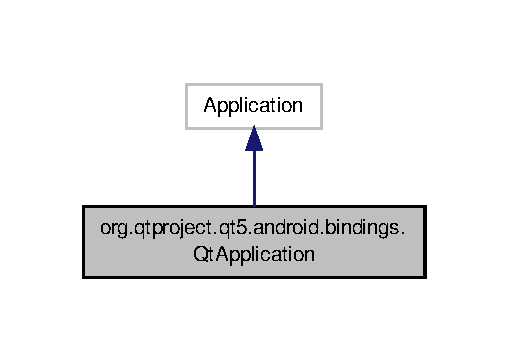
\includegraphics[width=244pt]{classorg_1_1qtproject_1_1qt5_1_1android_1_1bindings_1_1_qt_application__inherit__graph}
\end{center}
\end{figure}


Graphe de collaboration de org.\-qtproject.\-qt5.\-android.\-bindings.\-Qt\-Application\-:\nopagebreak
\begin{figure}[H]
\begin{center}
\leavevmode
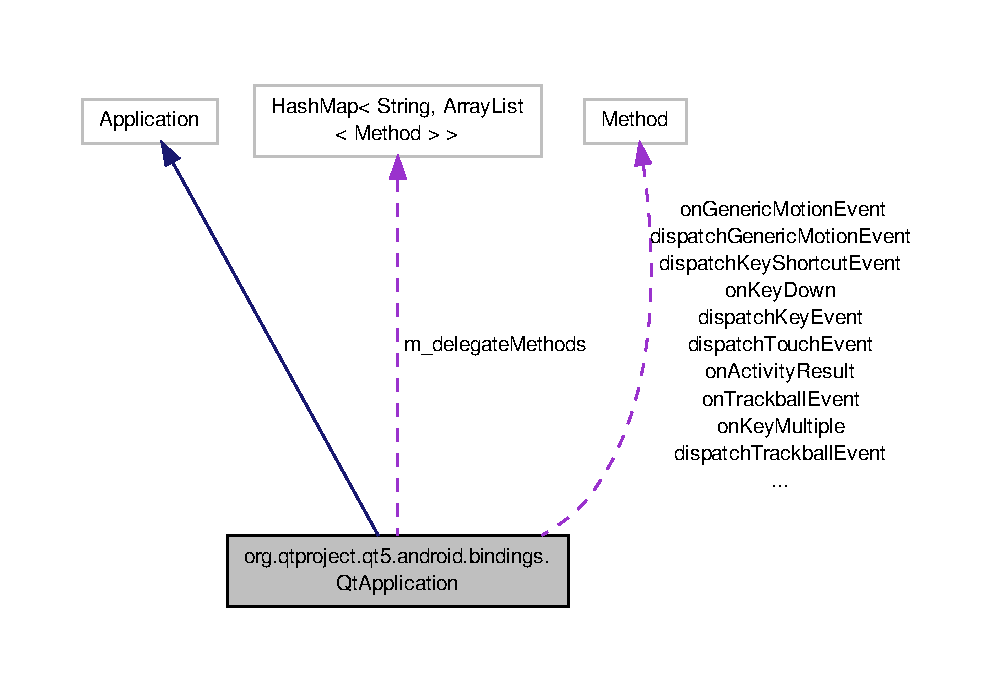
\includegraphics[width=350pt]{classorg_1_1qtproject_1_1qt5_1_1android_1_1bindings_1_1_qt_application__coll__graph}
\end{center}
\end{figure}
\subsection*{Classes}
\begin{DoxyCompactItemize}
\item 
class {\bfseries Invoke\-Result}
\end{DoxyCompactItemize}
\subsection*{Fonctions membres publiques}
\begin{DoxyCompactItemize}
\item 
void \hyperlink{classorg_1_1qtproject_1_1qt5_1_1android_1_1bindings_1_1_qt_application_a643840ad1a423ebcae10f20c6dcf98d0}{on\-Terminate} ()
\end{DoxyCompactItemize}
\subsection*{Fonctions membres publiques statiques}
\begin{DoxyCompactItemize}
\item 
static void \hyperlink{classorg_1_1qtproject_1_1qt5_1_1android_1_1bindings_1_1_qt_application_ac47f64e358a18d99b3f41756fe4a7849}{set\-Qt\-Activity\-Delegate} (Object listener)
\item 
static Invoke\-Result \hyperlink{classorg_1_1qtproject_1_1qt5_1_1android_1_1bindings_1_1_qt_application_a8e4549506cfd078644266970e25dd1c5}{invoke\-Delegate} (Object...\-args)
\item 
static Object \hyperlink{classorg_1_1qtproject_1_1qt5_1_1android_1_1bindings_1_1_qt_application_a2c90af718c6bbd962d96589337a754ea}{invoke\-Delegate\-Method} (Method m, Object...\-args)
\end{DoxyCompactItemize}
\subsection*{Attributs publics statiques}
\begin{DoxyCompactItemize}
\item 
static final String \hyperlink{classorg_1_1qtproject_1_1qt5_1_1android_1_1bindings_1_1_qt_application_acf8f3131e19aaef5fc2079bc530f42d6}{Qt\-T\-A\-G} = \char`\"{}Qt\char`\"{}
\item 
static Object \hyperlink{classorg_1_1qtproject_1_1qt5_1_1android_1_1bindings_1_1_qt_application_a8b778a94cf5468dfc07ae8f3e8d81148}{m\-\_\-delegate\-Object} = null
\item 
static Hash\-Map$<$ String, \\*
Array\-List$<$ Method $>$ $>$ \hyperlink{classorg_1_1qtproject_1_1qt5_1_1android_1_1bindings_1_1_qt_application_a5b32c9d8ce150fc1866812b13debbcfb}{m\-\_\-delegate\-Methods} = new Hash\-Map$<$String, Array\-List$<$Method$>$$>$()
\item 
static Method \hyperlink{classorg_1_1qtproject_1_1qt5_1_1android_1_1bindings_1_1_qt_application_a970719713bf7310b041b31dd6415fdcb}{dispatch\-Key\-Event} = null
\item 
static Method \hyperlink{classorg_1_1qtproject_1_1qt5_1_1android_1_1bindings_1_1_qt_application_a263117be3577f4976dc349a550cdb73f}{dispatch\-Populate\-Accessibility\-Event} = null
\item 
static Method \hyperlink{classorg_1_1qtproject_1_1qt5_1_1android_1_1bindings_1_1_qt_application_aa76cf4fe4b2ccebdca957464b7411745}{dispatch\-Touch\-Event} = null
\item 
static Method \hyperlink{classorg_1_1qtproject_1_1qt5_1_1android_1_1bindings_1_1_qt_application_acb66b3d0eafb07d1f13fb0a7ca4262bf}{dispatch\-Trackball\-Event} = null
\item 
static Method \hyperlink{classorg_1_1qtproject_1_1qt5_1_1android_1_1bindings_1_1_qt_application_a399e0ef76371331edc6aca47b4936dc6}{on\-Key\-Down} = null
\item 
static Method \hyperlink{classorg_1_1qtproject_1_1qt5_1_1android_1_1bindings_1_1_qt_application_a7098736b29503c41026ff60cca904094}{on\-Key\-Multiple} = null
\item 
static Method \hyperlink{classorg_1_1qtproject_1_1qt5_1_1android_1_1bindings_1_1_qt_application_a947623196f7f382c1c2bf0737697082d}{on\-Key\-Up} = null
\item 
static Method \hyperlink{classorg_1_1qtproject_1_1qt5_1_1android_1_1bindings_1_1_qt_application_ad8a6d1d7da859063ec8e5ba5b3db06c1}{on\-Touch\-Event} = null
\item 
static Method \hyperlink{classorg_1_1qtproject_1_1qt5_1_1android_1_1bindings_1_1_qt_application_aba0550a56d08380fb00cef9cc1a276d1}{on\-Trackball\-Event} = null
\item 
static Method \hyperlink{classorg_1_1qtproject_1_1qt5_1_1android_1_1bindings_1_1_qt_application_a6538f4bbf7fdf3a1eba5971bb830af71}{on\-Activity\-Result} = null
\item 
static Method \hyperlink{classorg_1_1qtproject_1_1qt5_1_1android_1_1bindings_1_1_qt_application_a2bd84d3f02531e21ab7434cd4d48b849}{on\-Create} = null
\item 
static Method \hyperlink{classorg_1_1qtproject_1_1qt5_1_1android_1_1bindings_1_1_qt_application_abe105cb7eb9d98af229bcc706ad7660b}{on\-Key\-Long\-Press} = null
\item 
static Method \hyperlink{classorg_1_1qtproject_1_1qt5_1_1android_1_1bindings_1_1_qt_application_aa2fb7f374d9a03d6b939375933ff5149}{dispatch\-Key\-Shortcut\-Event} = null
\item 
static Method \hyperlink{classorg_1_1qtproject_1_1qt5_1_1android_1_1bindings_1_1_qt_application_a1ce0a33219f8c6103b216ed433ceeefe}{on\-Key\-Shortcut} = null
\item 
static Method \hyperlink{classorg_1_1qtproject_1_1qt5_1_1android_1_1bindings_1_1_qt_application_a2c2d0ff311ded8aaa6dabdde99632a6c}{dispatch\-Generic\-Motion\-Event} = null
\item 
static Method \hyperlink{classorg_1_1qtproject_1_1qt5_1_1android_1_1bindings_1_1_qt_application_a2ba7755a97e7fadf952401719ca1f8e4}{on\-Generic\-Motion\-Event} = null
\end{DoxyCompactItemize}


\subsection{Description détaillée}


Définition à la ligne 36 du fichier Qt\-Application.\-java.



\subsection{Documentation des fonctions membres}
\hypertarget{classorg_1_1qtproject_1_1qt5_1_1android_1_1bindings_1_1_qt_application_a8e4549506cfd078644266970e25dd1c5}{\index{org\-::qtproject\-::qt5\-::android\-::bindings\-::\-Qt\-Application@{org\-::qtproject\-::qt5\-::android\-::bindings\-::\-Qt\-Application}!invoke\-Delegate@{invoke\-Delegate}}
\index{invoke\-Delegate@{invoke\-Delegate}!org::qtproject::qt5::android::bindings::QtApplication@{org\-::qtproject\-::qt5\-::android\-::bindings\-::\-Qt\-Application}}
\subsubsection[{invoke\-Delegate}]{\setlength{\rightskip}{0pt plus 5cm}static Invoke\-Result org.\-qtproject.\-qt5.\-android.\-bindings.\-Qt\-Application.\-invoke\-Delegate (
\begin{DoxyParamCaption}
\item[{Object...}]{args}
\end{DoxyParamCaption}
)\hspace{0.3cm}{\ttfamily [inline]}, {\ttfamily [static]}}}\label{classorg_1_1qtproject_1_1qt5_1_1android_1_1bindings_1_1_qt_application_a8e4549506cfd078644266970e25dd1c5}


Définition à la ligne 112 du fichier Qt\-Application.\-java.

\hypertarget{classorg_1_1qtproject_1_1qt5_1_1android_1_1bindings_1_1_qt_application_a2c90af718c6bbd962d96589337a754ea}{\index{org\-::qtproject\-::qt5\-::android\-::bindings\-::\-Qt\-Application@{org\-::qtproject\-::qt5\-::android\-::bindings\-::\-Qt\-Application}!invoke\-Delegate\-Method@{invoke\-Delegate\-Method}}
\index{invoke\-Delegate\-Method@{invoke\-Delegate\-Method}!org::qtproject::qt5::android::bindings::QtApplication@{org\-::qtproject\-::qt5\-::android\-::bindings\-::\-Qt\-Application}}
\subsubsection[{invoke\-Delegate\-Method}]{\setlength{\rightskip}{0pt plus 5cm}static Object org.\-qtproject.\-qt5.\-android.\-bindings.\-Qt\-Application.\-invoke\-Delegate\-Method (
\begin{DoxyParamCaption}
\item[{Method}]{m, }
\item[{Object...}]{args}
\end{DoxyParamCaption}
)\hspace{0.3cm}{\ttfamily [inline]}, {\ttfamily [static]}}}\label{classorg_1_1qtproject_1_1qt5_1_1android_1_1bindings_1_1_qt_application_a2c90af718c6bbd962d96589337a754ea}


Définition à la ligne 140 du fichier Qt\-Application.\-java.

\hypertarget{classorg_1_1qtproject_1_1qt5_1_1android_1_1bindings_1_1_qt_application_a643840ad1a423ebcae10f20c6dcf98d0}{\index{org\-::qtproject\-::qt5\-::android\-::bindings\-::\-Qt\-Application@{org\-::qtproject\-::qt5\-::android\-::bindings\-::\-Qt\-Application}!on\-Terminate@{on\-Terminate}}
\index{on\-Terminate@{on\-Terminate}!org::qtproject::qt5::android::bindings::QtApplication@{org\-::qtproject\-::qt5\-::android\-::bindings\-::\-Qt\-Application}}
\subsubsection[{on\-Terminate}]{\setlength{\rightskip}{0pt plus 5cm}void org.\-qtproject.\-qt5.\-android.\-bindings.\-Qt\-Application.\-on\-Terminate (
\begin{DoxyParamCaption}
{}
\end{DoxyParamCaption}
)\hspace{0.3cm}{\ttfamily [inline]}}}\label{classorg_1_1qtproject_1_1qt5_1_1android_1_1bindings_1_1_qt_application_a643840ad1a423ebcae10f20c6dcf98d0}


Définition à la ligne 99 du fichier Qt\-Application.\-java.

\hypertarget{classorg_1_1qtproject_1_1qt5_1_1android_1_1bindings_1_1_qt_application_ac47f64e358a18d99b3f41756fe4a7849}{\index{org\-::qtproject\-::qt5\-::android\-::bindings\-::\-Qt\-Application@{org\-::qtproject\-::qt5\-::android\-::bindings\-::\-Qt\-Application}!set\-Qt\-Activity\-Delegate@{set\-Qt\-Activity\-Delegate}}
\index{set\-Qt\-Activity\-Delegate@{set\-Qt\-Activity\-Delegate}!org::qtproject::qt5::android::bindings::QtApplication@{org\-::qtproject\-::qt5\-::android\-::bindings\-::\-Qt\-Application}}
\subsubsection[{set\-Qt\-Activity\-Delegate}]{\setlength{\rightskip}{0pt plus 5cm}static void org.\-qtproject.\-qt5.\-android.\-bindings.\-Qt\-Application.\-set\-Qt\-Activity\-Delegate (
\begin{DoxyParamCaption}
\item[{Object}]{listener}
\end{DoxyParamCaption}
)\hspace{0.3cm}{\ttfamily [inline]}, {\ttfamily [static]}}}\label{classorg_1_1qtproject_1_1qt5_1_1android_1_1bindings_1_1_qt_application_ac47f64e358a18d99b3f41756fe4a7849}


Définition à la ligne 58 du fichier Qt\-Application.\-java.



\subsection{Documentation des données membres}
\hypertarget{classorg_1_1qtproject_1_1qt5_1_1android_1_1bindings_1_1_qt_application_a2c2d0ff311ded8aaa6dabdde99632a6c}{\index{org\-::qtproject\-::qt5\-::android\-::bindings\-::\-Qt\-Application@{org\-::qtproject\-::qt5\-::android\-::bindings\-::\-Qt\-Application}!dispatch\-Generic\-Motion\-Event@{dispatch\-Generic\-Motion\-Event}}
\index{dispatch\-Generic\-Motion\-Event@{dispatch\-Generic\-Motion\-Event}!org::qtproject::qt5::android::bindings::QtApplication@{org\-::qtproject\-::qt5\-::android\-::bindings\-::\-Qt\-Application}}
\subsubsection[{dispatch\-Generic\-Motion\-Event}]{\setlength{\rightskip}{0pt plus 5cm}Method org.\-qtproject.\-qt5.\-android.\-bindings.\-Qt\-Application.\-dispatch\-Generic\-Motion\-Event = null\hspace{0.3cm}{\ttfamily [static]}}}\label{classorg_1_1qtproject_1_1qt5_1_1android_1_1bindings_1_1_qt_application_a2c2d0ff311ded8aaa6dabdde99632a6c}


Définition à la ligne 55 du fichier Qt\-Application.\-java.

\hypertarget{classorg_1_1qtproject_1_1qt5_1_1android_1_1bindings_1_1_qt_application_a970719713bf7310b041b31dd6415fdcb}{\index{org\-::qtproject\-::qt5\-::android\-::bindings\-::\-Qt\-Application@{org\-::qtproject\-::qt5\-::android\-::bindings\-::\-Qt\-Application}!dispatch\-Key\-Event@{dispatch\-Key\-Event}}
\index{dispatch\-Key\-Event@{dispatch\-Key\-Event}!org::qtproject::qt5::android::bindings::QtApplication@{org\-::qtproject\-::qt5\-::android\-::bindings\-::\-Qt\-Application}}
\subsubsection[{dispatch\-Key\-Event}]{\setlength{\rightskip}{0pt plus 5cm}Method org.\-qtproject.\-qt5.\-android.\-bindings.\-Qt\-Application.\-dispatch\-Key\-Event = null\hspace{0.3cm}{\ttfamily [static]}}}\label{classorg_1_1qtproject_1_1qt5_1_1android_1_1bindings_1_1_qt_application_a970719713bf7310b041b31dd6415fdcb}


Définition à la ligne 41 du fichier Qt\-Application.\-java.

\hypertarget{classorg_1_1qtproject_1_1qt5_1_1android_1_1bindings_1_1_qt_application_aa2fb7f374d9a03d6b939375933ff5149}{\index{org\-::qtproject\-::qt5\-::android\-::bindings\-::\-Qt\-Application@{org\-::qtproject\-::qt5\-::android\-::bindings\-::\-Qt\-Application}!dispatch\-Key\-Shortcut\-Event@{dispatch\-Key\-Shortcut\-Event}}
\index{dispatch\-Key\-Shortcut\-Event@{dispatch\-Key\-Shortcut\-Event}!org::qtproject::qt5::android::bindings::QtApplication@{org\-::qtproject\-::qt5\-::android\-::bindings\-::\-Qt\-Application}}
\subsubsection[{dispatch\-Key\-Shortcut\-Event}]{\setlength{\rightskip}{0pt plus 5cm}Method org.\-qtproject.\-qt5.\-android.\-bindings.\-Qt\-Application.\-dispatch\-Key\-Shortcut\-Event = null\hspace{0.3cm}{\ttfamily [static]}}}\label{classorg_1_1qtproject_1_1qt5_1_1android_1_1bindings_1_1_qt_application_aa2fb7f374d9a03d6b939375933ff5149}


Définition à la ligne 53 du fichier Qt\-Application.\-java.

\hypertarget{classorg_1_1qtproject_1_1qt5_1_1android_1_1bindings_1_1_qt_application_a263117be3577f4976dc349a550cdb73f}{\index{org\-::qtproject\-::qt5\-::android\-::bindings\-::\-Qt\-Application@{org\-::qtproject\-::qt5\-::android\-::bindings\-::\-Qt\-Application}!dispatch\-Populate\-Accessibility\-Event@{dispatch\-Populate\-Accessibility\-Event}}
\index{dispatch\-Populate\-Accessibility\-Event@{dispatch\-Populate\-Accessibility\-Event}!org::qtproject::qt5::android::bindings::QtApplication@{org\-::qtproject\-::qt5\-::android\-::bindings\-::\-Qt\-Application}}
\subsubsection[{dispatch\-Populate\-Accessibility\-Event}]{\setlength{\rightskip}{0pt plus 5cm}Method org.\-qtproject.\-qt5.\-android.\-bindings.\-Qt\-Application.\-dispatch\-Populate\-Accessibility\-Event = null\hspace{0.3cm}{\ttfamily [static]}}}\label{classorg_1_1qtproject_1_1qt5_1_1android_1_1bindings_1_1_qt_application_a263117be3577f4976dc349a550cdb73f}


Définition à la ligne 42 du fichier Qt\-Application.\-java.

\hypertarget{classorg_1_1qtproject_1_1qt5_1_1android_1_1bindings_1_1_qt_application_aa76cf4fe4b2ccebdca957464b7411745}{\index{org\-::qtproject\-::qt5\-::android\-::bindings\-::\-Qt\-Application@{org\-::qtproject\-::qt5\-::android\-::bindings\-::\-Qt\-Application}!dispatch\-Touch\-Event@{dispatch\-Touch\-Event}}
\index{dispatch\-Touch\-Event@{dispatch\-Touch\-Event}!org::qtproject::qt5::android::bindings::QtApplication@{org\-::qtproject\-::qt5\-::android\-::bindings\-::\-Qt\-Application}}
\subsubsection[{dispatch\-Touch\-Event}]{\setlength{\rightskip}{0pt plus 5cm}Method org.\-qtproject.\-qt5.\-android.\-bindings.\-Qt\-Application.\-dispatch\-Touch\-Event = null\hspace{0.3cm}{\ttfamily [static]}}}\label{classorg_1_1qtproject_1_1qt5_1_1android_1_1bindings_1_1_qt_application_aa76cf4fe4b2ccebdca957464b7411745}


Définition à la ligne 43 du fichier Qt\-Application.\-java.

\hypertarget{classorg_1_1qtproject_1_1qt5_1_1android_1_1bindings_1_1_qt_application_acb66b3d0eafb07d1f13fb0a7ca4262bf}{\index{org\-::qtproject\-::qt5\-::android\-::bindings\-::\-Qt\-Application@{org\-::qtproject\-::qt5\-::android\-::bindings\-::\-Qt\-Application}!dispatch\-Trackball\-Event@{dispatch\-Trackball\-Event}}
\index{dispatch\-Trackball\-Event@{dispatch\-Trackball\-Event}!org::qtproject::qt5::android::bindings::QtApplication@{org\-::qtproject\-::qt5\-::android\-::bindings\-::\-Qt\-Application}}
\subsubsection[{dispatch\-Trackball\-Event}]{\setlength{\rightskip}{0pt plus 5cm}Method org.\-qtproject.\-qt5.\-android.\-bindings.\-Qt\-Application.\-dispatch\-Trackball\-Event = null\hspace{0.3cm}{\ttfamily [static]}}}\label{classorg_1_1qtproject_1_1qt5_1_1android_1_1bindings_1_1_qt_application_acb66b3d0eafb07d1f13fb0a7ca4262bf}


Définition à la ligne 44 du fichier Qt\-Application.\-java.

\hypertarget{classorg_1_1qtproject_1_1qt5_1_1android_1_1bindings_1_1_qt_application_a5b32c9d8ce150fc1866812b13debbcfb}{\index{org\-::qtproject\-::qt5\-::android\-::bindings\-::\-Qt\-Application@{org\-::qtproject\-::qt5\-::android\-::bindings\-::\-Qt\-Application}!m\-\_\-delegate\-Methods@{m\-\_\-delegate\-Methods}}
\index{m\-\_\-delegate\-Methods@{m\-\_\-delegate\-Methods}!org::qtproject::qt5::android::bindings::QtApplication@{org\-::qtproject\-::qt5\-::android\-::bindings\-::\-Qt\-Application}}
\subsubsection[{m\-\_\-delegate\-Methods}]{\setlength{\rightskip}{0pt plus 5cm}Hash\-Map$<$String, Array\-List$<$Method$>$ $>$ org.\-qtproject.\-qt5.\-android.\-bindings.\-Qt\-Application.\-m\-\_\-delegate\-Methods = new Hash\-Map$<$String, Array\-List$<$Method$>$$>$()\hspace{0.3cm}{\ttfamily [static]}}}\label{classorg_1_1qtproject_1_1qt5_1_1android_1_1bindings_1_1_qt_application_a5b32c9d8ce150fc1866812b13debbcfb}


Définition à la ligne 40 du fichier Qt\-Application.\-java.

\hypertarget{classorg_1_1qtproject_1_1qt5_1_1android_1_1bindings_1_1_qt_application_a8b778a94cf5468dfc07ae8f3e8d81148}{\index{org\-::qtproject\-::qt5\-::android\-::bindings\-::\-Qt\-Application@{org\-::qtproject\-::qt5\-::android\-::bindings\-::\-Qt\-Application}!m\-\_\-delegate\-Object@{m\-\_\-delegate\-Object}}
\index{m\-\_\-delegate\-Object@{m\-\_\-delegate\-Object}!org::qtproject::qt5::android::bindings::QtApplication@{org\-::qtproject\-::qt5\-::android\-::bindings\-::\-Qt\-Application}}
\subsubsection[{m\-\_\-delegate\-Object}]{\setlength{\rightskip}{0pt plus 5cm}Object org.\-qtproject.\-qt5.\-android.\-bindings.\-Qt\-Application.\-m\-\_\-delegate\-Object = null\hspace{0.3cm}{\ttfamily [static]}}}\label{classorg_1_1qtproject_1_1qt5_1_1android_1_1bindings_1_1_qt_application_a8b778a94cf5468dfc07ae8f3e8d81148}


Définition à la ligne 39 du fichier Qt\-Application.\-java.

\hypertarget{classorg_1_1qtproject_1_1qt5_1_1android_1_1bindings_1_1_qt_application_a6538f4bbf7fdf3a1eba5971bb830af71}{\index{org\-::qtproject\-::qt5\-::android\-::bindings\-::\-Qt\-Application@{org\-::qtproject\-::qt5\-::android\-::bindings\-::\-Qt\-Application}!on\-Activity\-Result@{on\-Activity\-Result}}
\index{on\-Activity\-Result@{on\-Activity\-Result}!org::qtproject::qt5::android::bindings::QtApplication@{org\-::qtproject\-::qt5\-::android\-::bindings\-::\-Qt\-Application}}
\subsubsection[{on\-Activity\-Result}]{\setlength{\rightskip}{0pt plus 5cm}Method org.\-qtproject.\-qt5.\-android.\-bindings.\-Qt\-Application.\-on\-Activity\-Result = null\hspace{0.3cm}{\ttfamily [static]}}}\label{classorg_1_1qtproject_1_1qt5_1_1android_1_1bindings_1_1_qt_application_a6538f4bbf7fdf3a1eba5971bb830af71}


Définition à la ligne 50 du fichier Qt\-Application.\-java.

\hypertarget{classorg_1_1qtproject_1_1qt5_1_1android_1_1bindings_1_1_qt_application_a2bd84d3f02531e21ab7434cd4d48b849}{\index{org\-::qtproject\-::qt5\-::android\-::bindings\-::\-Qt\-Application@{org\-::qtproject\-::qt5\-::android\-::bindings\-::\-Qt\-Application}!on\-Create@{on\-Create}}
\index{on\-Create@{on\-Create}!org::qtproject::qt5::android::bindings::QtApplication@{org\-::qtproject\-::qt5\-::android\-::bindings\-::\-Qt\-Application}}
\subsubsection[{on\-Create}]{\setlength{\rightskip}{0pt plus 5cm}Method org.\-qtproject.\-qt5.\-android.\-bindings.\-Qt\-Application.\-on\-Create = null\hspace{0.3cm}{\ttfamily [static]}}}\label{classorg_1_1qtproject_1_1qt5_1_1android_1_1bindings_1_1_qt_application_a2bd84d3f02531e21ab7434cd4d48b849}


Définition à la ligne 51 du fichier Qt\-Application.\-java.

\hypertarget{classorg_1_1qtproject_1_1qt5_1_1android_1_1bindings_1_1_qt_application_a2ba7755a97e7fadf952401719ca1f8e4}{\index{org\-::qtproject\-::qt5\-::android\-::bindings\-::\-Qt\-Application@{org\-::qtproject\-::qt5\-::android\-::bindings\-::\-Qt\-Application}!on\-Generic\-Motion\-Event@{on\-Generic\-Motion\-Event}}
\index{on\-Generic\-Motion\-Event@{on\-Generic\-Motion\-Event}!org::qtproject::qt5::android::bindings::QtApplication@{org\-::qtproject\-::qt5\-::android\-::bindings\-::\-Qt\-Application}}
\subsubsection[{on\-Generic\-Motion\-Event}]{\setlength{\rightskip}{0pt plus 5cm}Method org.\-qtproject.\-qt5.\-android.\-bindings.\-Qt\-Application.\-on\-Generic\-Motion\-Event = null\hspace{0.3cm}{\ttfamily [static]}}}\label{classorg_1_1qtproject_1_1qt5_1_1android_1_1bindings_1_1_qt_application_a2ba7755a97e7fadf952401719ca1f8e4}


Définition à la ligne 56 du fichier Qt\-Application.\-java.

\hypertarget{classorg_1_1qtproject_1_1qt5_1_1android_1_1bindings_1_1_qt_application_a399e0ef76371331edc6aca47b4936dc6}{\index{org\-::qtproject\-::qt5\-::android\-::bindings\-::\-Qt\-Application@{org\-::qtproject\-::qt5\-::android\-::bindings\-::\-Qt\-Application}!on\-Key\-Down@{on\-Key\-Down}}
\index{on\-Key\-Down@{on\-Key\-Down}!org::qtproject::qt5::android::bindings::QtApplication@{org\-::qtproject\-::qt5\-::android\-::bindings\-::\-Qt\-Application}}
\subsubsection[{on\-Key\-Down}]{\setlength{\rightskip}{0pt plus 5cm}Method org.\-qtproject.\-qt5.\-android.\-bindings.\-Qt\-Application.\-on\-Key\-Down = null\hspace{0.3cm}{\ttfamily [static]}}}\label{classorg_1_1qtproject_1_1qt5_1_1android_1_1bindings_1_1_qt_application_a399e0ef76371331edc6aca47b4936dc6}


Définition à la ligne 45 du fichier Qt\-Application.\-java.

\hypertarget{classorg_1_1qtproject_1_1qt5_1_1android_1_1bindings_1_1_qt_application_abe105cb7eb9d98af229bcc706ad7660b}{\index{org\-::qtproject\-::qt5\-::android\-::bindings\-::\-Qt\-Application@{org\-::qtproject\-::qt5\-::android\-::bindings\-::\-Qt\-Application}!on\-Key\-Long\-Press@{on\-Key\-Long\-Press}}
\index{on\-Key\-Long\-Press@{on\-Key\-Long\-Press}!org::qtproject::qt5::android::bindings::QtApplication@{org\-::qtproject\-::qt5\-::android\-::bindings\-::\-Qt\-Application}}
\subsubsection[{on\-Key\-Long\-Press}]{\setlength{\rightskip}{0pt plus 5cm}Method org.\-qtproject.\-qt5.\-android.\-bindings.\-Qt\-Application.\-on\-Key\-Long\-Press = null\hspace{0.3cm}{\ttfamily [static]}}}\label{classorg_1_1qtproject_1_1qt5_1_1android_1_1bindings_1_1_qt_application_abe105cb7eb9d98af229bcc706ad7660b}


Définition à la ligne 52 du fichier Qt\-Application.\-java.

\hypertarget{classorg_1_1qtproject_1_1qt5_1_1android_1_1bindings_1_1_qt_application_a7098736b29503c41026ff60cca904094}{\index{org\-::qtproject\-::qt5\-::android\-::bindings\-::\-Qt\-Application@{org\-::qtproject\-::qt5\-::android\-::bindings\-::\-Qt\-Application}!on\-Key\-Multiple@{on\-Key\-Multiple}}
\index{on\-Key\-Multiple@{on\-Key\-Multiple}!org::qtproject::qt5::android::bindings::QtApplication@{org\-::qtproject\-::qt5\-::android\-::bindings\-::\-Qt\-Application}}
\subsubsection[{on\-Key\-Multiple}]{\setlength{\rightskip}{0pt plus 5cm}Method org.\-qtproject.\-qt5.\-android.\-bindings.\-Qt\-Application.\-on\-Key\-Multiple = null\hspace{0.3cm}{\ttfamily [static]}}}\label{classorg_1_1qtproject_1_1qt5_1_1android_1_1bindings_1_1_qt_application_a7098736b29503c41026ff60cca904094}


Définition à la ligne 46 du fichier Qt\-Application.\-java.

\hypertarget{classorg_1_1qtproject_1_1qt5_1_1android_1_1bindings_1_1_qt_application_a1ce0a33219f8c6103b216ed433ceeefe}{\index{org\-::qtproject\-::qt5\-::android\-::bindings\-::\-Qt\-Application@{org\-::qtproject\-::qt5\-::android\-::bindings\-::\-Qt\-Application}!on\-Key\-Shortcut@{on\-Key\-Shortcut}}
\index{on\-Key\-Shortcut@{on\-Key\-Shortcut}!org::qtproject::qt5::android::bindings::QtApplication@{org\-::qtproject\-::qt5\-::android\-::bindings\-::\-Qt\-Application}}
\subsubsection[{on\-Key\-Shortcut}]{\setlength{\rightskip}{0pt plus 5cm}Method org.\-qtproject.\-qt5.\-android.\-bindings.\-Qt\-Application.\-on\-Key\-Shortcut = null\hspace{0.3cm}{\ttfamily [static]}}}\label{classorg_1_1qtproject_1_1qt5_1_1android_1_1bindings_1_1_qt_application_a1ce0a33219f8c6103b216ed433ceeefe}


Définition à la ligne 54 du fichier Qt\-Application.\-java.

\hypertarget{classorg_1_1qtproject_1_1qt5_1_1android_1_1bindings_1_1_qt_application_a947623196f7f382c1c2bf0737697082d}{\index{org\-::qtproject\-::qt5\-::android\-::bindings\-::\-Qt\-Application@{org\-::qtproject\-::qt5\-::android\-::bindings\-::\-Qt\-Application}!on\-Key\-Up@{on\-Key\-Up}}
\index{on\-Key\-Up@{on\-Key\-Up}!org::qtproject::qt5::android::bindings::QtApplication@{org\-::qtproject\-::qt5\-::android\-::bindings\-::\-Qt\-Application}}
\subsubsection[{on\-Key\-Up}]{\setlength{\rightskip}{0pt plus 5cm}Method org.\-qtproject.\-qt5.\-android.\-bindings.\-Qt\-Application.\-on\-Key\-Up = null\hspace{0.3cm}{\ttfamily [static]}}}\label{classorg_1_1qtproject_1_1qt5_1_1android_1_1bindings_1_1_qt_application_a947623196f7f382c1c2bf0737697082d}


Définition à la ligne 47 du fichier Qt\-Application.\-java.

\hypertarget{classorg_1_1qtproject_1_1qt5_1_1android_1_1bindings_1_1_qt_application_ad8a6d1d7da859063ec8e5ba5b3db06c1}{\index{org\-::qtproject\-::qt5\-::android\-::bindings\-::\-Qt\-Application@{org\-::qtproject\-::qt5\-::android\-::bindings\-::\-Qt\-Application}!on\-Touch\-Event@{on\-Touch\-Event}}
\index{on\-Touch\-Event@{on\-Touch\-Event}!org::qtproject::qt5::android::bindings::QtApplication@{org\-::qtproject\-::qt5\-::android\-::bindings\-::\-Qt\-Application}}
\subsubsection[{on\-Touch\-Event}]{\setlength{\rightskip}{0pt plus 5cm}Method org.\-qtproject.\-qt5.\-android.\-bindings.\-Qt\-Application.\-on\-Touch\-Event = null\hspace{0.3cm}{\ttfamily [static]}}}\label{classorg_1_1qtproject_1_1qt5_1_1android_1_1bindings_1_1_qt_application_ad8a6d1d7da859063ec8e5ba5b3db06c1}


Définition à la ligne 48 du fichier Qt\-Application.\-java.

\hypertarget{classorg_1_1qtproject_1_1qt5_1_1android_1_1bindings_1_1_qt_application_aba0550a56d08380fb00cef9cc1a276d1}{\index{org\-::qtproject\-::qt5\-::android\-::bindings\-::\-Qt\-Application@{org\-::qtproject\-::qt5\-::android\-::bindings\-::\-Qt\-Application}!on\-Trackball\-Event@{on\-Trackball\-Event}}
\index{on\-Trackball\-Event@{on\-Trackball\-Event}!org::qtproject::qt5::android::bindings::QtApplication@{org\-::qtproject\-::qt5\-::android\-::bindings\-::\-Qt\-Application}}
\subsubsection[{on\-Trackball\-Event}]{\setlength{\rightskip}{0pt plus 5cm}Method org.\-qtproject.\-qt5.\-android.\-bindings.\-Qt\-Application.\-on\-Trackball\-Event = null\hspace{0.3cm}{\ttfamily [static]}}}\label{classorg_1_1qtproject_1_1qt5_1_1android_1_1bindings_1_1_qt_application_aba0550a56d08380fb00cef9cc1a276d1}


Définition à la ligne 49 du fichier Qt\-Application.\-java.

\hypertarget{classorg_1_1qtproject_1_1qt5_1_1android_1_1bindings_1_1_qt_application_acf8f3131e19aaef5fc2079bc530f42d6}{\index{org\-::qtproject\-::qt5\-::android\-::bindings\-::\-Qt\-Application@{org\-::qtproject\-::qt5\-::android\-::bindings\-::\-Qt\-Application}!Qt\-T\-A\-G@{Qt\-T\-A\-G}}
\index{Qt\-T\-A\-G@{Qt\-T\-A\-G}!org::qtproject::qt5::android::bindings::QtApplication@{org\-::qtproject\-::qt5\-::android\-::bindings\-::\-Qt\-Application}}
\subsubsection[{Qt\-T\-A\-G}]{\setlength{\rightskip}{0pt plus 5cm}final String org.\-qtproject.\-qt5.\-android.\-bindings.\-Qt\-Application.\-Qt\-T\-A\-G = \char`\"{}Qt\char`\"{}\hspace{0.3cm}{\ttfamily [static]}}}\label{classorg_1_1qtproject_1_1qt5_1_1android_1_1bindings_1_1_qt_application_acf8f3131e19aaef5fc2079bc530f42d6}


Définition à la ligne 38 du fichier Qt\-Application.\-java.



La documentation de cette classe a été générée à partir du fichier suivant \-:\begin{DoxyCompactItemize}
\item 
android/src/org/qtproject/qt5/android/bindings/\hyperlink{_qt_application_8java}{Qt\-Application.\-java}\end{DoxyCompactItemize}

\chapter{Documentation des fichiers}
\hypertarget{_qt_activity_8java}{\section{Référence du fichier android/src/org/qtproject/qt5/android/bindings/\-Qt\-Activity.java}
\label{_qt_activity_8java}\index{android/src/org/qtproject/qt5/android/bindings/\-Qt\-Activity.\-java@{android/src/org/qtproject/qt5/android/bindings/\-Qt\-Activity.\-java}}
}
\subsection*{Classes}
\begin{DoxyCompactItemize}
\item 
class \hyperlink{classorg_1_1qtproject_1_1qt5_1_1android_1_1bindings_1_1_qt_activity}{org.\-qtproject.\-qt5.\-android.\-bindings.\-Qt\-Activity}
\end{DoxyCompactItemize}
\subsection*{Espaces de nommage}
\begin{DoxyCompactItemize}
\item 
package \hyperlink{namespaceorg_1_1qtproject_1_1qt5_1_1android_1_1bindings}{org.\-qtproject.\-qt5.\-android.\-bindings}
\end{DoxyCompactItemize}

\hypertarget{_qt_application_8java}{\section{Référence du fichier android/src/org/qtproject/qt5/android/bindings/\-Qt\-Application.java}
\label{_qt_application_8java}\index{android/src/org/qtproject/qt5/android/bindings/\-Qt\-Application.\-java@{android/src/org/qtproject/qt5/android/bindings/\-Qt\-Application.\-java}}
}
\subsection*{Classes}
\begin{DoxyCompactItemize}
\item 
class \hyperlink{classorg_1_1qtproject_1_1qt5_1_1android_1_1bindings_1_1_qt_application}{org.\-qtproject.\-qt5.\-android.\-bindings.\-Qt\-Application}
\item 
class {\bfseries org.\-qtproject.\-qt5.\-android.\-bindings.\-Qt\-Application.\-Invoke\-Result}
\end{DoxyCompactItemize}
\subsection*{Espaces de nommage}
\begin{DoxyCompactItemize}
\item 
package \hyperlink{namespaceorg_1_1qtproject_1_1qt5_1_1android_1_1bindings}{org.\-qtproject.\-qt5.\-android.\-bindings}
\end{DoxyCompactItemize}

\hypertarget{emplacement_8cpp}{\section{Référence du fichier emplacement.\-cpp}
\label{emplacement_8cpp}\index{emplacement.\-cpp@{emplacement.\-cpp}}
}
{\ttfamily \#include \char`\"{}emplacement.\-h\char`\"{}}\\*
{\ttfamily \#include $<$Q\-Debug$>$}\\*
{\ttfamily \#include $<$Q\-Painter$>$}\\*
{\ttfamily \#include $<$Q\-Status\-Bar$>$}\\*
{\ttfamily \#include $<$Q\-Mouse\-Event$>$}\\*
Graphe des dépendances par inclusion de emplacement.\-cpp\-:\nopagebreak
\begin{figure}[H]
\begin{center}
\leavevmode
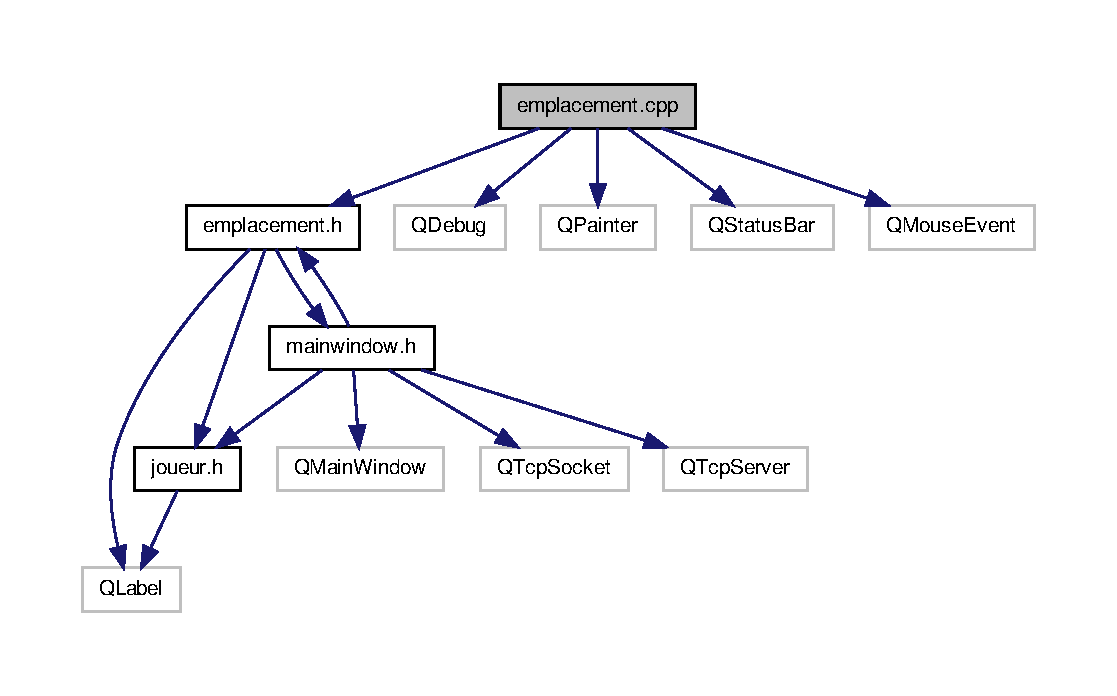
\includegraphics[width=350pt]{emplacement_8cpp__incl}
\end{center}
\end{figure}

\hypertarget{emplacement_8h}{\section{Référence du fichier emplacement.\-h}
\label{emplacement_8h}\index{emplacement.\-h@{emplacement.\-h}}
}
{\ttfamily \#include $<$Q\-Label$>$}\\*
{\ttfamily \#include \char`\"{}mainwindow.\-h\char`\"{}}\\*
{\ttfamily \#include \char`\"{}joueur.\-h\char`\"{}}\\*
Graphe des dépendances par inclusion de emplacement.\-h\-:\nopagebreak
\begin{figure}[H]
\begin{center}
\leavevmode
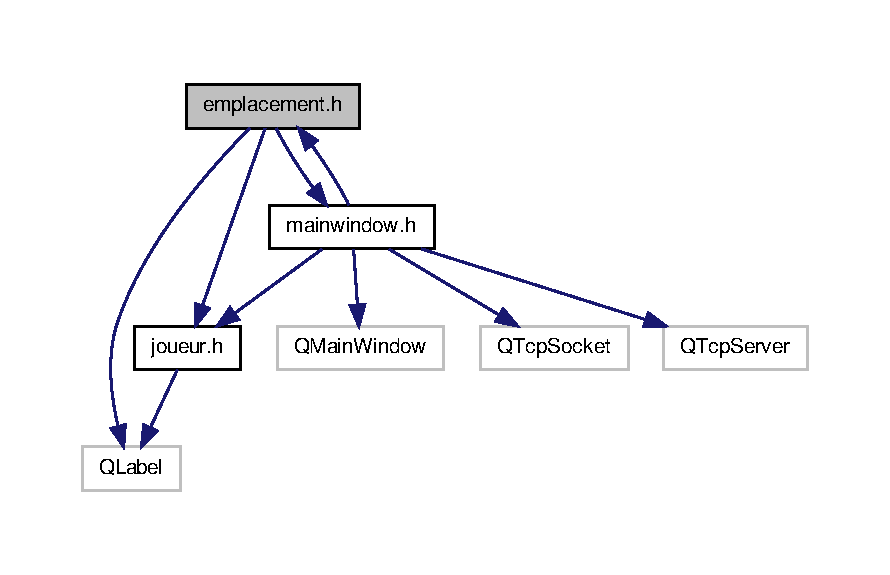
\includegraphics[width=350pt]{emplacement_8h__incl}
\end{center}
\end{figure}
Ce graphe montre quels fichiers incluent directement ou indirectement ce fichier \-:\nopagebreak
\begin{figure}[H]
\begin{center}
\leavevmode
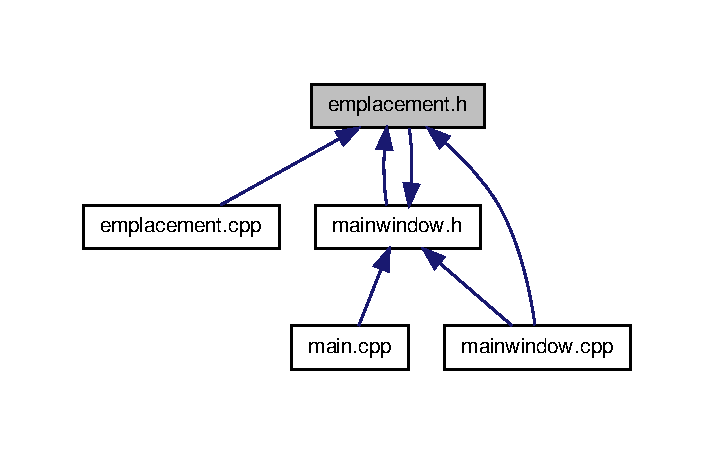
\includegraphics[width=342pt]{emplacement_8h__dep__incl}
\end{center}
\end{figure}
\subsection*{Classes}
\begin{DoxyCompactItemize}
\item 
class \hyperlink{classemplacement}{emplacement}
\begin{DoxyCompactList}\small\item\em The emplacement class. \end{DoxyCompactList}\end{DoxyCompactItemize}

\hypertarget{help_8cpp}{\section{Référence du fichier help.\-cpp}
\label{help_8cpp}\index{help.\-cpp@{help.\-cpp}}
}
{\ttfamily \#include \char`\"{}help.\-h\char`\"{}}\\*
{\ttfamily \#include \char`\"{}ui\-\_\-help.\-h\char`\"{}}\\*
Graphe des dépendances par inclusion de help.\-cpp\-:\nopagebreak
\begin{figure}[H]
\begin{center}
\leavevmode
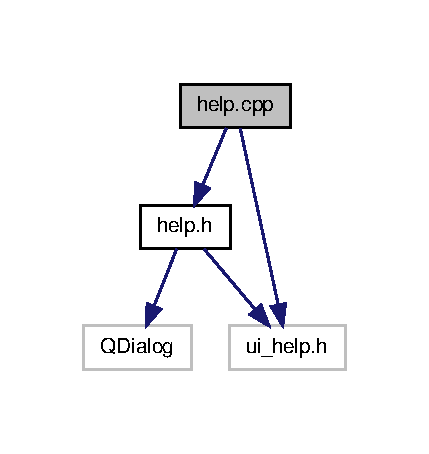
\includegraphics[width=206pt]{help_8cpp__incl}
\end{center}
\end{figure}

\hypertarget{help_8h}{\section{Référence du fichier help.\-h}
\label{help_8h}\index{help.\-h@{help.\-h}}
}
{\ttfamily \#include $<$Q\-Dialog$>$}\\*
{\ttfamily \#include $<$ui\-\_\-help.\-h$>$}\\*
Graphe des dépendances par inclusion de help.\-h\-:\nopagebreak
\begin{figure}[H]
\begin{center}
\leavevmode
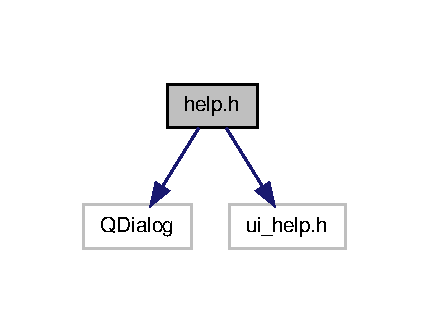
\includegraphics[width=206pt]{help_8h__incl}
\end{center}
\end{figure}
Ce graphe montre quels fichiers incluent directement ou indirectement ce fichier \-:\nopagebreak
\begin{figure}[H]
\begin{center}
\leavevmode
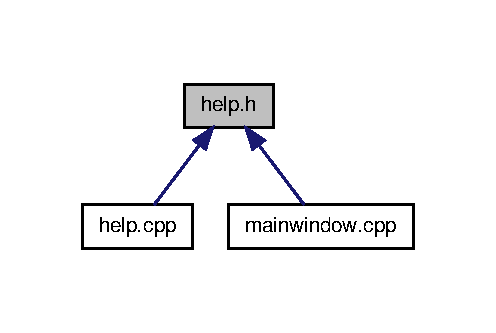
\includegraphics[width=238pt]{help_8h__dep__incl}
\end{center}
\end{figure}
\subsection*{Classes}
\begin{DoxyCompactItemize}
\item 
class \hyperlink{classhelp}{help}
\begin{DoxyCompactList}\small\item\em The help class. \end{DoxyCompactList}\end{DoxyCompactItemize}
\subsection*{Espaces de nommage}
\begin{DoxyCompactItemize}
\item 
namespace \hyperlink{namespace_ui}{Ui}
\begin{DoxyCompactList}\small\item\em Classe help \char`\"{}help.\-h\char`\"{}. \end{DoxyCompactList}\end{DoxyCompactItemize}

\hypertarget{joueur_8cpp}{\section{Référence du fichier joueur.\-cpp}
\label{joueur_8cpp}\index{joueur.\-cpp@{joueur.\-cpp}}
}
{\ttfamily \#include \char`\"{}joueur.\-h\char`\"{}}\\*
{\ttfamily \#include $<$Q\-Painter$>$}\\*
Graphe des dépendances par inclusion de joueur.\-cpp\-:\nopagebreak
\begin{figure}[H]
\begin{center}
\leavevmode
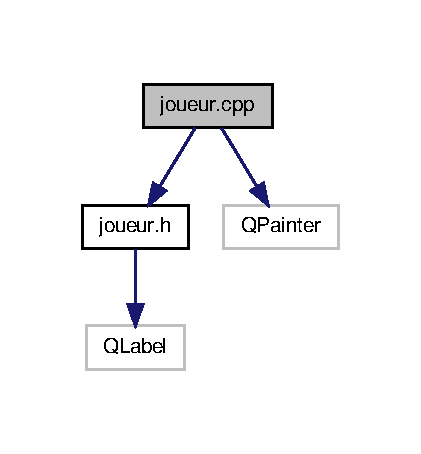
\includegraphics[width=202pt]{joueur_8cpp__incl}
\end{center}
\end{figure}

\hypertarget{joueur_8h}{\section{Référence du fichier joueur.\-h}
\label{joueur_8h}\index{joueur.\-h@{joueur.\-h}}
}
{\ttfamily \#include $<$Q\-Label$>$}\\*
Graphe des dépendances par inclusion de joueur.\-h\-:\nopagebreak
\begin{figure}[H]
\begin{center}
\leavevmode
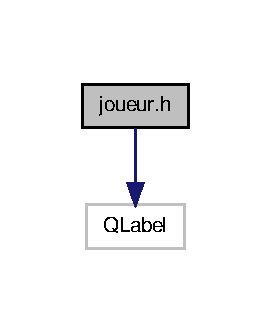
\includegraphics[width=130pt]{joueur_8h__incl}
\end{center}
\end{figure}
Ce graphe montre quels fichiers incluent directement ou indirectement ce fichier \-:\nopagebreak
\begin{figure}[H]
\begin{center}
\leavevmode
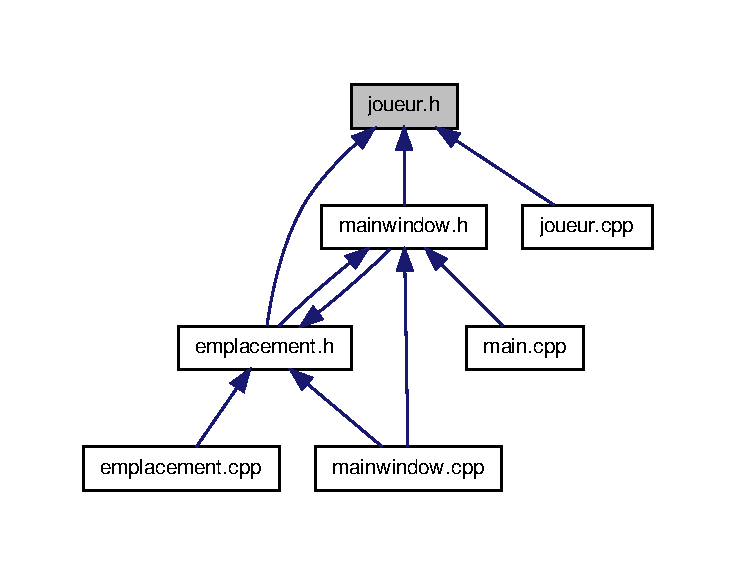
\includegraphics[width=350pt]{joueur_8h__dep__incl}
\end{center}
\end{figure}
\subsection*{Classes}
\begin{DoxyCompactItemize}
\item 
class \hyperlink{classjoueur}{joueur}
\begin{DoxyCompactList}\small\item\em Classe joueur \char`\"{}joueur.\-h\char`\"{}. \end{DoxyCompactList}\end{DoxyCompactItemize}

\hypertarget{main_8cpp}{\section{Référence du fichier main.\-cpp}
\label{main_8cpp}\index{main.\-cpp@{main.\-cpp}}
}
{\ttfamily \#include \char`\"{}mainwindow.\-h\char`\"{}}\\*
{\ttfamily \#include $<$Q\-Application$>$}\\*
{\ttfamily \#include $<$Q\-Translator$>$}\\*
{\ttfamily \#include $<$Q\-File$>$}\\*
{\ttfamily \#include $<$Q\-Debug$>$}\\*
Graphe des dépendances par inclusion de main.\-cpp\-:\nopagebreak
\begin{figure}[H]
\begin{center}
\leavevmode
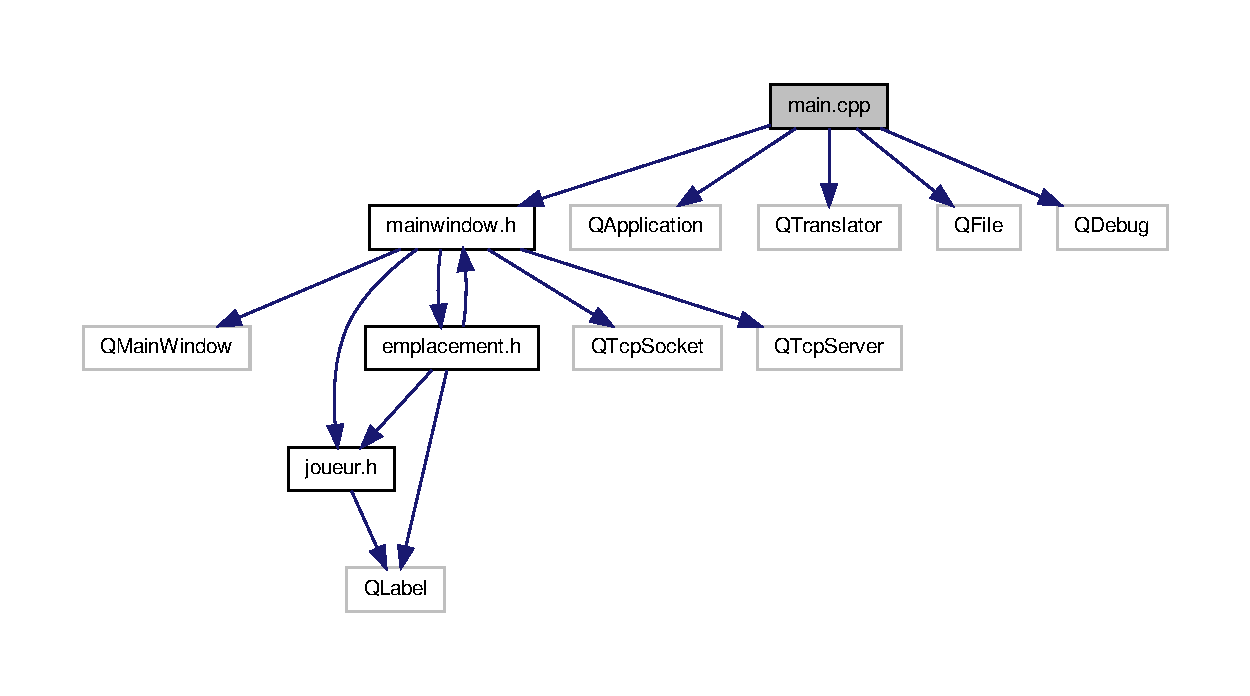
\includegraphics[width=350pt]{main_8cpp__incl}
\end{center}
\end{figure}
\subsection*{Fonctions}
\begin{DoxyCompactItemize}
\item 
int \hyperlink{main_8cpp_a0ddf1224851353fc92bfbff6f499fa97}{main} (int argc, char $\ast$argv\mbox{[}$\,$\mbox{]})
\end{DoxyCompactItemize}


\subsection{Documentation des fonctions}
\hypertarget{main_8cpp_a0ddf1224851353fc92bfbff6f499fa97}{\index{main.\-cpp@{main.\-cpp}!main@{main}}
\index{main@{main}!main.cpp@{main.\-cpp}}
\subsubsection[{main}]{\setlength{\rightskip}{0pt plus 5cm}int main (
\begin{DoxyParamCaption}
\item[{int}]{argc, }
\item[{char $\ast$}]{argv\mbox{[}$\,$\mbox{]}}
\end{DoxyParamCaption}
)}}\label{main_8cpp_a0ddf1224851353fc92bfbff6f499fa97}


Définition à la ligne 6 du fichier main.\-cpp.


\hypertarget{mainwindow_8cpp}{\section{Référence du fichier mainwindow.\-cpp}
\label{mainwindow_8cpp}\index{mainwindow.\-cpp@{mainwindow.\-cpp}}
}
{\ttfamily \#include \char`\"{}mainwindow.\-h\char`\"{}}\\*
{\ttfamily \#include \char`\"{}ui\-\_\-mainwindow.\-h\char`\"{}}\\*
{\ttfamily \#include \char`\"{}emplacement.\-h\char`\"{}}\\*
{\ttfamily \#include $<$Q\-Status\-Bar$>$}\\*
{\ttfamily \#include $<$Q\-Timer$>$}\\*
{\ttfamily \#include $<$Q\-Input\-Dialog$>$}\\*
{\ttfamily \#include $<$Q\-Debug$>$}\\*
{\ttfamily \#include $<$help.\-h$>$}\\*
{\ttfamily \#include $<$ui\-\_\-help.\-h$>$}\\*
Graphe des dépendances par inclusion de mainwindow.\-cpp\-:\nopagebreak
\begin{figure}[H]
\begin{center}
\leavevmode
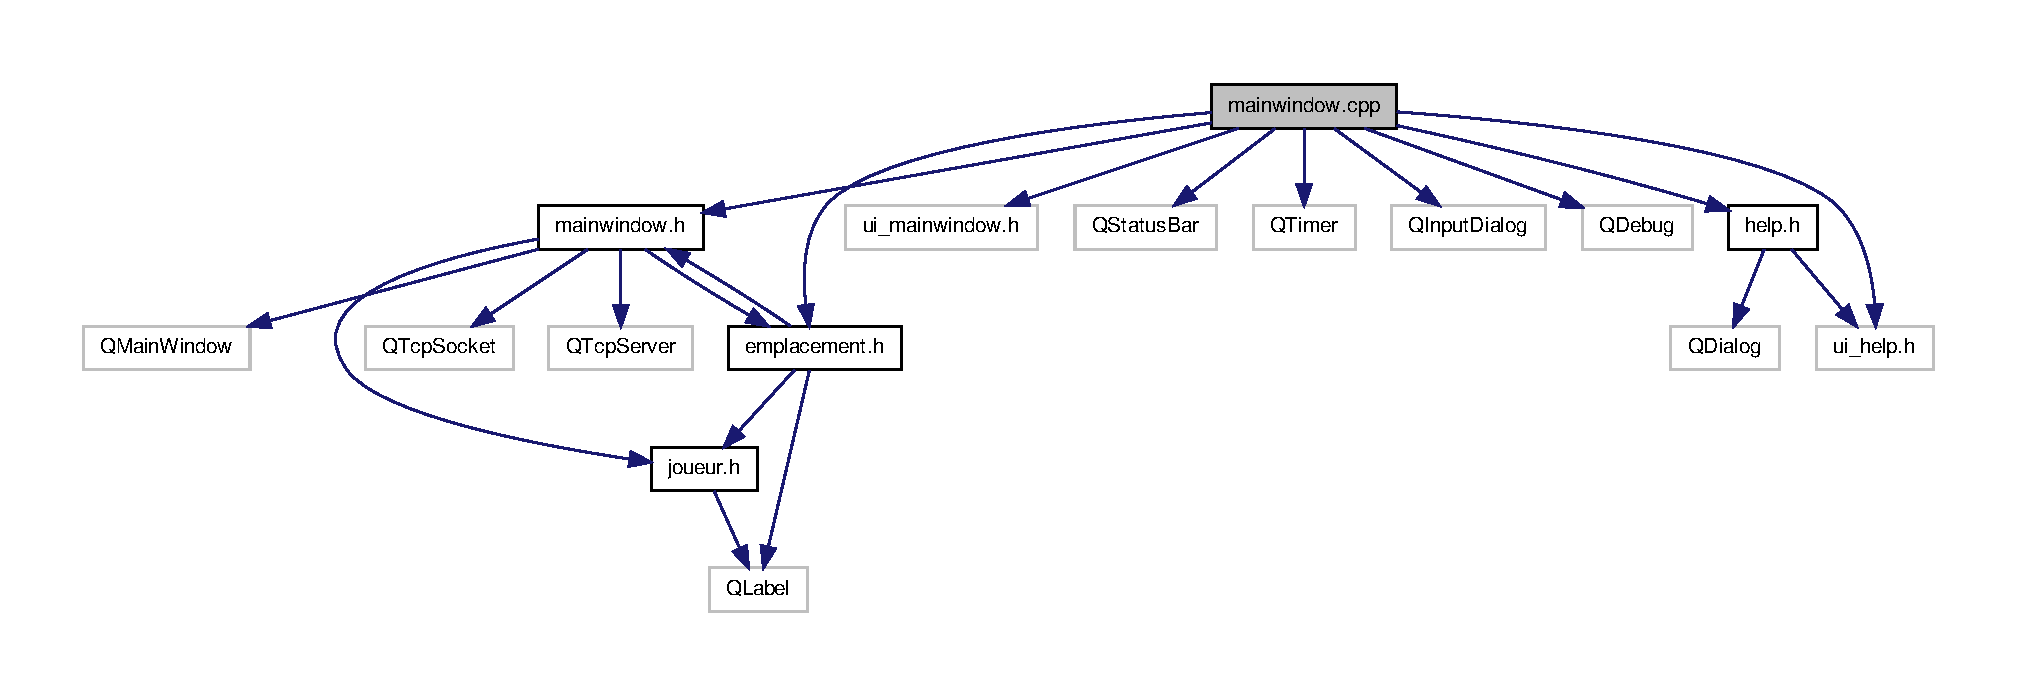
\includegraphics[width=350pt]{mainwindow_8cpp__incl}
\end{center}
\end{figure}

\hypertarget{mainwindow_8h}{\section{Référence du fichier mainwindow.\-h}
\label{mainwindow_8h}\index{mainwindow.\-h@{mainwindow.\-h}}
}
{\ttfamily \#include $<$Q\-Main\-Window$>$}\\*
{\ttfamily \#include \char`\"{}joueur.\-h\char`\"{}}\\*
{\ttfamily \#include \char`\"{}emplacement.\-h\char`\"{}}\\*
{\ttfamily \#include $<$Q\-Tcp\-Socket$>$}\\*
{\ttfamily \#include $<$Q\-Tcp\-Server$>$}\\*
Graphe des dépendances par inclusion de mainwindow.\-h\-:\nopagebreak
\begin{figure}[H]
\begin{center}
\leavevmode
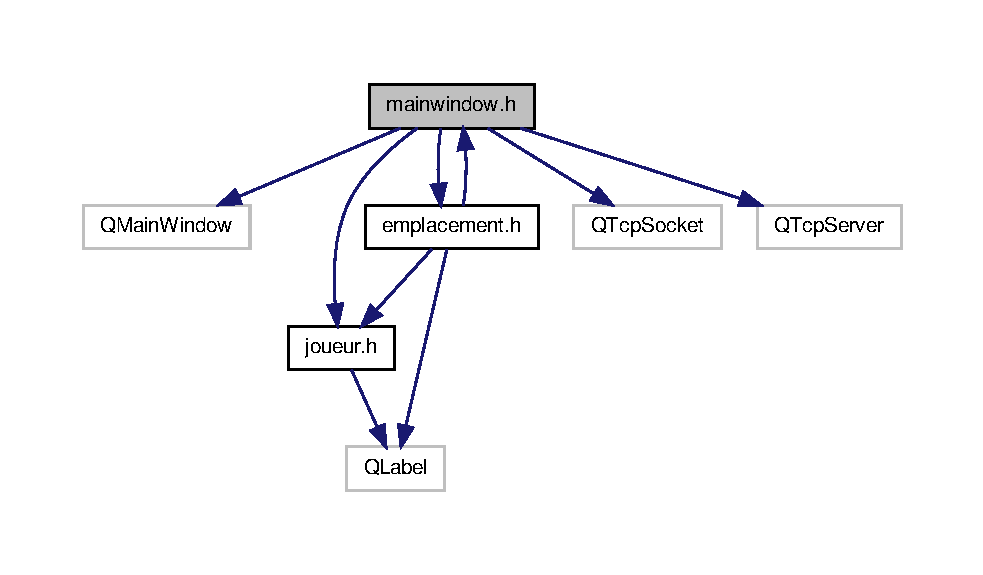
\includegraphics[width=350pt]{mainwindow_8h__incl}
\end{center}
\end{figure}
Ce graphe montre quels fichiers incluent directement ou indirectement ce fichier \-:\nopagebreak
\begin{figure}[H]
\begin{center}
\leavevmode
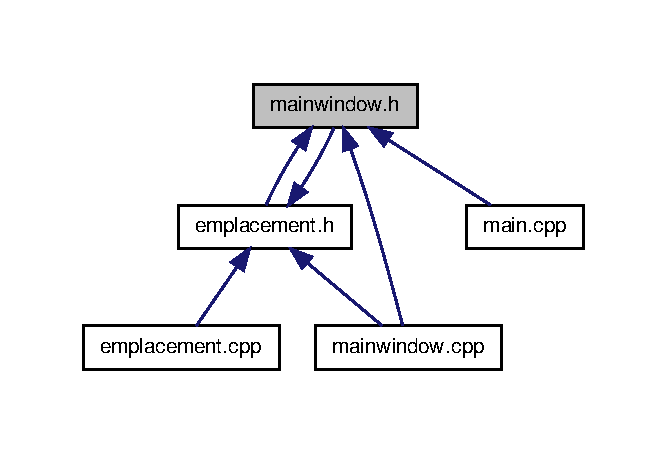
\includegraphics[width=320pt]{mainwindow_8h__dep__incl}
\end{center}
\end{figure}
\subsection*{Classes}
\begin{DoxyCompactItemize}
\item 
class \hyperlink{class_main_window}{Main\-Window}
\begin{DoxyCompactList}\small\item\em The \hyperlink{class_main_window}{Main\-Window} class. \end{DoxyCompactList}\end{DoxyCompactItemize}
\subsection*{Espaces de nommage}
\begin{DoxyCompactItemize}
\item 
namespace \hyperlink{namespace_ui}{Ui}
\begin{DoxyCompactList}\small\item\em Classe help \char`\"{}help.\-h\char`\"{}. \end{DoxyCompactList}\end{DoxyCompactItemize}

\printindex
\end{document}
